% Options for packages loaded elsewhere
\PassOptionsToPackage{unicode}{hyperref}
\PassOptionsToPackage{hyphens}{url}
%
\documentclass[
]{book}
\usepackage{lmodern}
\usepackage{amsmath}
\usepackage{ifxetex,ifluatex}
\ifnum 0\ifxetex 1\fi\ifluatex 1\fi=0 % if pdftex
  \usepackage[T1]{fontenc}
  \usepackage[utf8]{inputenc}
  \usepackage{textcomp} % provide euro and other symbols
  \usepackage{amssymb}
\else % if luatex or xetex
  \usepackage{unicode-math}
  \defaultfontfeatures{Scale=MatchLowercase}
  \defaultfontfeatures[\rmfamily]{Ligatures=TeX,Scale=1}
\fi
% Use upquote if available, for straight quotes in verbatim environments
\IfFileExists{upquote.sty}{\usepackage{upquote}}{}
\IfFileExists{microtype.sty}{% use microtype if available
  \usepackage[]{microtype}
  \UseMicrotypeSet[protrusion]{basicmath} % disable protrusion for tt fonts
}{}
\makeatletter
\@ifundefined{KOMAClassName}{% if non-KOMA class
  \IfFileExists{parskip.sty}{%
    \usepackage{parskip}
  }{% else
    \setlength{\parindent}{0pt}
    \setlength{\parskip}{6pt plus 2pt minus 1pt}}
}{% if KOMA class
  \KOMAoptions{parskip=half}}
\makeatother
\usepackage{xcolor}
\IfFileExists{xurl.sty}{\usepackage{xurl}}{} % add URL line breaks if available
\IfFileExists{bookmark.sty}{\usepackage{bookmark}}{\usepackage{hyperref}}
\hypersetup{
  pdftitle={Data analysis using R for Psychology},
  pdfauthor={Alexander (Sasha) Pastukhov},
  hidelinks,
  pdfcreator={LaTeX via pandoc}}
\urlstyle{same} % disable monospaced font for URLs
\usepackage{color}
\usepackage{fancyvrb}
\newcommand{\VerbBar}{|}
\newcommand{\VERB}{\Verb[commandchars=\\\{\}]}
\DefineVerbatimEnvironment{Highlighting}{Verbatim}{commandchars=\\\{\}}
% Add ',fontsize=\small' for more characters per line
\usepackage{framed}
\definecolor{shadecolor}{RGB}{248,248,248}
\newenvironment{Shaded}{\begin{snugshade}}{\end{snugshade}}
\newcommand{\AlertTok}[1]{\textcolor[rgb]{0.94,0.16,0.16}{#1}}
\newcommand{\AnnotationTok}[1]{\textcolor[rgb]{0.56,0.35,0.01}{\textbf{\textit{#1}}}}
\newcommand{\AttributeTok}[1]{\textcolor[rgb]{0.77,0.63,0.00}{#1}}
\newcommand{\BaseNTok}[1]{\textcolor[rgb]{0.00,0.00,0.81}{#1}}
\newcommand{\BuiltInTok}[1]{#1}
\newcommand{\CharTok}[1]{\textcolor[rgb]{0.31,0.60,0.02}{#1}}
\newcommand{\CommentTok}[1]{\textcolor[rgb]{0.56,0.35,0.01}{\textit{#1}}}
\newcommand{\CommentVarTok}[1]{\textcolor[rgb]{0.56,0.35,0.01}{\textbf{\textit{#1}}}}
\newcommand{\ConstantTok}[1]{\textcolor[rgb]{0.00,0.00,0.00}{#1}}
\newcommand{\ControlFlowTok}[1]{\textcolor[rgb]{0.13,0.29,0.53}{\textbf{#1}}}
\newcommand{\DataTypeTok}[1]{\textcolor[rgb]{0.13,0.29,0.53}{#1}}
\newcommand{\DecValTok}[1]{\textcolor[rgb]{0.00,0.00,0.81}{#1}}
\newcommand{\DocumentationTok}[1]{\textcolor[rgb]{0.56,0.35,0.01}{\textbf{\textit{#1}}}}
\newcommand{\ErrorTok}[1]{\textcolor[rgb]{0.64,0.00,0.00}{\textbf{#1}}}
\newcommand{\ExtensionTok}[1]{#1}
\newcommand{\FloatTok}[1]{\textcolor[rgb]{0.00,0.00,0.81}{#1}}
\newcommand{\FunctionTok}[1]{\textcolor[rgb]{0.00,0.00,0.00}{#1}}
\newcommand{\ImportTok}[1]{#1}
\newcommand{\InformationTok}[1]{\textcolor[rgb]{0.56,0.35,0.01}{\textbf{\textit{#1}}}}
\newcommand{\KeywordTok}[1]{\textcolor[rgb]{0.13,0.29,0.53}{\textbf{#1}}}
\newcommand{\NormalTok}[1]{#1}
\newcommand{\OperatorTok}[1]{\textcolor[rgb]{0.81,0.36,0.00}{\textbf{#1}}}
\newcommand{\OtherTok}[1]{\textcolor[rgb]{0.56,0.35,0.01}{#1}}
\newcommand{\PreprocessorTok}[1]{\textcolor[rgb]{0.56,0.35,0.01}{\textit{#1}}}
\newcommand{\RegionMarkerTok}[1]{#1}
\newcommand{\SpecialCharTok}[1]{\textcolor[rgb]{0.00,0.00,0.00}{#1}}
\newcommand{\SpecialStringTok}[1]{\textcolor[rgb]{0.31,0.60,0.02}{#1}}
\newcommand{\StringTok}[1]{\textcolor[rgb]{0.31,0.60,0.02}{#1}}
\newcommand{\VariableTok}[1]{\textcolor[rgb]{0.00,0.00,0.00}{#1}}
\newcommand{\VerbatimStringTok}[1]{\textcolor[rgb]{0.31,0.60,0.02}{#1}}
\newcommand{\WarningTok}[1]{\textcolor[rgb]{0.56,0.35,0.01}{\textbf{\textit{#1}}}}
\usepackage{longtable,booktabs}
% Correct order of tables after \paragraph or \subparagraph
\usepackage{etoolbox}
\makeatletter
\patchcmd\longtable{\par}{\if@noskipsec\mbox{}\fi\par}{}{}
\makeatother
% Allow footnotes in longtable head/foot
\IfFileExists{footnotehyper.sty}{\usepackage{footnotehyper}}{\usepackage{footnote}}
\makesavenoteenv{longtable}
\usepackage{graphicx}
\makeatletter
\def\maxwidth{\ifdim\Gin@nat@width>\linewidth\linewidth\else\Gin@nat@width\fi}
\def\maxheight{\ifdim\Gin@nat@height>\textheight\textheight\else\Gin@nat@height\fi}
\makeatother
% Scale images if necessary, so that they will not overflow the page
% margins by default, and it is still possible to overwrite the defaults
% using explicit options in \includegraphics[width, height, ...]{}
\setkeys{Gin}{width=\maxwidth,height=\maxheight,keepaspectratio}
% Set default figure placement to htbp
\makeatletter
\def\fps@figure{htbp}
\makeatother
\setlength{\emergencystretch}{3em} % prevent overfull lines
\providecommand{\tightlist}{%
  \setlength{\itemsep}{0pt}\setlength{\parskip}{0pt}}
\setcounter{secnumdepth}{5}
\usepackage{booktabs}
\ifluatex
  \usepackage{selnolig}  % disable illegal ligatures
\fi
\usepackage[]{natbib}
\bibliographystyle{apalike}

\title{Data analysis using R for Psychology}
\author{Alexander (Sasha) Pastukhov}
\date{2020-12-01}

\begin{document}
\maketitle

{
\setcounter{tocdepth}{1}
\tableofcontents
}
\hypertarget{introduction}{%
\chapter*{Introduction}\label{introduction}}
\addcontentsline{toc}{chapter}{Introduction}

This is a material for \emph{Applied data analysis for psychology using the open-source software R} seminar as taught at \href{https://www.uni-bamberg.de/psychologie/}{Institute of Psychology} at University of Bamberg.

This work is licensed under a Creative Commons Attribution-NonCommercial-ShareAlike 4.0 International License.

\hypertarget{about-the-seminar}{%
\section*{About the seminar}\label{about-the-seminar}}
\addcontentsline{toc}{section}{About the seminar}

Each chapter covers a single seminar, introducing necessary ideas and is accompanied by a notebook with exercises, which you need to complete and submit. The material assumes no foreknowledge of R or programming in general from the reader. Its purpose is to gradually build up your knowledge and introduce to a typical analysis pipeline. It is based on a data that is typical for the field (repeated measures, appearance, accuracy and response time measurements, Likert scale reports, etc.), you are welcome to suggest your own data set for analysis. Even if you already performed the analysis using some other program, it would still be insightful to compare the different ways and, perhaps, you might gain a new insight. Plus, it is more engaging to work on your data.

Remember that throughout the seminar you can and should(!) always ask me whenever something is unclear, you do not understand a concept or logic behind certain code. Do not hesitate to write me in the team or (better) directly to me in the chat (in the latter case, the notifications are harder miss and we don't spam others with our conversation).

You will need to submit your assignment one day before the next seminar (Tuesday before noon at the latest), so I would have time evaluate it and provide feedback.

As a final assignment, you will need to program a full analysis pipeline for a given data set (or, if you want, for your data set). All the necessary steps will be covered by the seminar material. Please inform me, If you require a grade, as then I will create a more specific description for you to have a clear understanding of how the program will be graded.

\hypertarget{content-of-the-seminar}{%
\section*{Content of the seminar}\label{content-of-the-seminar}}
\addcontentsline{toc}{section}{Content of the seminar}

The ultimate goal of the seminar is to give you tools to perform a complete analysis of a typical psychology research data, including data import and merging, pre-processing, aggregating, plotting, and performing statistical analysis. We will start with very basic R programming concepts (vectors, tables) before proceeding to learn about data import and visualization via \href{https://ggplot2.tidyverse.org/}{the grammar of graphics}. Next, we will learn about piping that makes sequential analysis easy to write and read. Then, we will see how combine piping with Tidyverse \emph{verbs}. Next, we will see how to use, visualize, and report statistical models. Finally, you will learn the power of functional programming that provides ultimate flexibility in R.

\hypertarget{note-on-exercises}{%
\section*{Note on exercises}\label{note-on-exercises}}
\addcontentsline{toc}{section}{Note on exercises}

In many exercises your will be not writing the code but reading and understanding it. Your job in this case is ``to think like a computer''. Your advantage is that computers are very dumb, so instructions for them must be written in very simple, clear, and unambiguous way. This means that, with practice, reading code is easy for a human (well, reading a well-written code is easy, you will eventually encounter ``spaghetti-code'' which is easier to rewrite from scratch than to understand). In each case, you simply go through the code line-by-line, doing all computations by hand and writing down values stored in the variables (if there are too many to keep track of). Once you go through the code in this manner, it should be completely transparent for you. No mysteries should remain, you should have no doubts or uncertainty about any(!) line. Moreover, you then can run the code and check that the values you are getting from computer match yours. Any difference means you made a mistake and code is working differently from how you think it does. In any case, \textbf{if you not 100\% sure about any line of code, ask me, so we can go through it together!}

In a sense, this is the most important programming skill. It is impossible to learn how to write, if you cannot read first! Moreover, when programming you will probably spend more time reading the code and making sure that it works correctly than writing the new code. Thus, use this opportunity to practice and never use the code that you do not understand completely. Thus, there is nothing wrong in using \href{https://stackoverflow.com/}{stackoverflow} but do make sure you understand the code you copied!

\hypertarget{why-r}{%
\section*{Why R?}\label{why-r}}
\addcontentsline{toc}{section}{Why R?}

There are many software tools that allow you preprocess, plot, and analyze your data. Some cost money (SPSS, Matlab), some are free just like R (Python, Julia). Moreover, you can replicate all the analysis that we will perform using Python in combination with \href{https://jupyter.org/}{Jupyter notebooks} (for reproducable analysis), \href{https://pandas.pydata.org/}{Pandas} (for Excel-style table) and \href{https://www.statsmodels.org/stable/index.html}{statmodels} (for statistical analysis). However, R in combination with piping and \href{https://www.tidyverse.org/}{Tidyverse} family of packages is optimized for data analysis, making it easy to write simple, powerful and expressive code that is very easy to understand (a huge plus, as you will discover). I will run circles around myself trying to replicate the same analysis in Python or Matlab. In addition, R is loved by mathematicians and statisticians, so it tends to have implementations for all cutting edge methods (my impression is that even Python is lagging behind it in that respect).

\hypertarget{tidyverse-versus-base-r}{%
\section*{Tidyverse versus base R}\label{tidyverse-versus-base-r}}
\addcontentsline{toc}{section}{Tidyverse versus base R}

I will be teaching what one might call a ``dialect'' of R, based on \href{https://www.tidyverse.org/}{Tidyverse} family of packages. R is extremely flexible, making it possible to redefine its own syntax. Because of that Tidyverse-based code is very different from the base R code to the point that it might look like written in a completely different language (which, in a sense, it is). Although Tidyverse, at least in my opinion, is a better way, we will start with \emph{base R}, so that you will be able to read and understand code written outside of Tidyverse, as it is also very common.

\hypertarget{getting-started}{%
\chapter*{Getting Started}\label{getting-started}}
\addcontentsline{toc}{chapter}{Getting Started}

\hypertarget{installing-r}{%
\section*{Installing R}\label{installing-r}}
\addcontentsline{toc}{section}{Installing R}

Go to \href{https://cloud.r-project.org/}{r-project.org} and download the current stable version of R for your platform. Run the installer, accepting all defaults. The installer will ask you whether you also want the 32-bit version to be installed alongside 64-bit. You probably won't need 32-bit, so if space is at premium you can skip it. Otherwise, it will make very little difference.

\hypertarget{installing-r-studio}{%
\section*{Installing R-Studio}\label{installing-r-studio}}
\addcontentsline{toc}{section}{Installing R-Studio}

Go to \href{https://rstudio.com/products/rstudio/download/}{rstudio.com} and download \emph{RStudio Desktop Free} edition for your platform. Install it using defaults. The \emph{R-Studio} is an integrated development environment for R but you need to install R separately first! The R-Studio will automatically detect latest R that you have and, in case you have several versions of R installed, you will be able to alter that choice.

I will explain the necessary details on using R-Studio throughout the seminar but the \href{https://github.com/rstudio/cheatsheets/raw/master/rstudio-ide.pdf}{official cheatsheet} is an excellent, compact, and up-to-date source of information. In fact, R Studio has numerous \href{https://rstudio.com/resources/cheatsheets/}{cheatsheets} that describe individual packages in a compact form.

\hypertarget{rtools}{%
\section*{Installing RTools}\label{rtools}}
\addcontentsline{toc}{section}{Installing RTools}

If you are using Windows, we might need \href{https://cran.r-project.org/bin/windows/Rtools/}{Rtools} for building and running some packages. You do not need to install it at the beginning, but when we will need it later, just following the link above, download the latest \emph{Rtools} version, run the installer using the defaults and \textbf{follow the instructions on that page to put Rtools on the PATH}! (I do not repeat them here, because they might change).

\hypertarget{install.packages}{%
\section*{Installing packages}\label{install.packages}}
\addcontentsline{toc}{section}{Installing packages}

The real power of R lies in a vast community-driven family of packages suitable for any occasion. The default repository used by R and R-Studio is \href{https://cran.r-project.org/}{The Comprehensive R Archive Network} (a.k.a. \emph{CRAN}). It has very strict requirements for submitted packages, which makes it very annoying for the authors but ensures high quality. Most packages are well-documented and come with example data and code. We will use CRAN as a sole source for packages, but there are alternatives, such as \href{http://www.bioconductor.org/}{Bioconductor} that might have a package that is missing at CRAN. The Bioconductor relies on its own package manager, so you will need to consult the latest manual on their website.

To install CRAN package you have two alternatives: via command line function or via R-Studio package manager interface (which will call the function for you). In the former case, go to \texttt{Console} tab and type \texttt{install.packages("package-name")}, for example \texttt{install.packages("tidyverse")}, and press \texttt{Enter}.

\begin{center}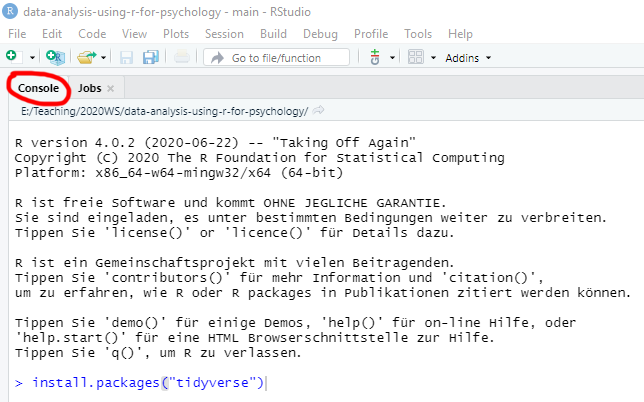
\includegraphics[width=1\linewidth]{images/install-packages-cmd} \end{center}

Alternatively, go to \texttt{Packages} tab, click on \texttt{Install} button, enter the package name in the window, which has autocomplete to help you, and press \texttt{Install}.

\begin{center}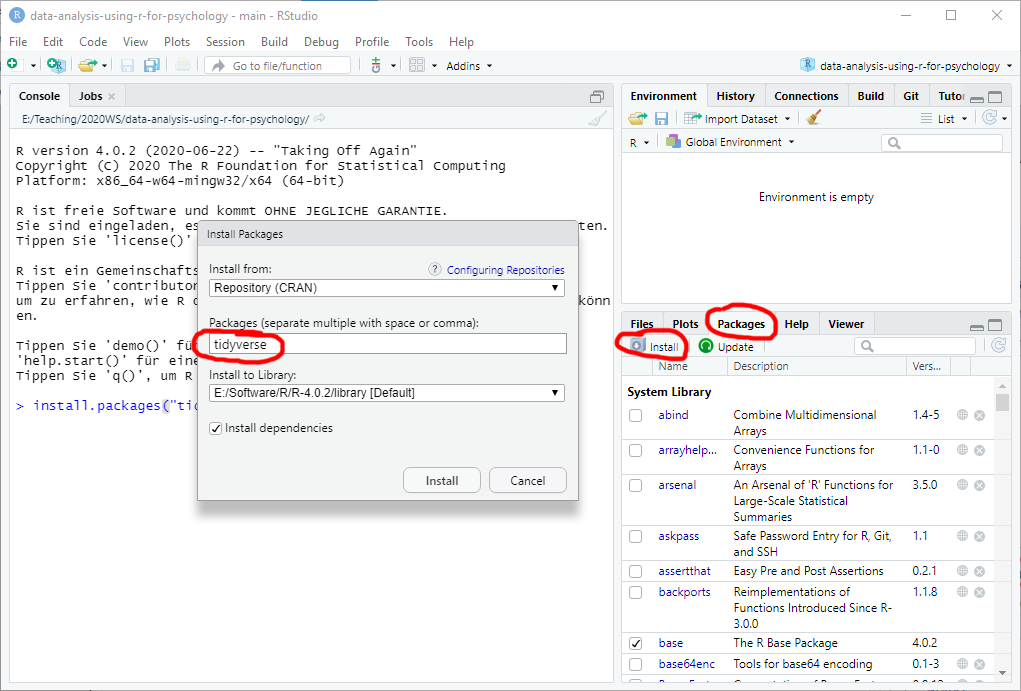
\includegraphics[width=1\linewidth]{images/install-packages-gui} \end{center}

In some cases, R will ask whether you want to install packages from source. In this case, it will grab the source code and compile the package, which takes time and requires \protect\hyperlink{rtools}{RTools}. In most cases, you can say ``No'' to install a pre-build binary version. The binary version will be slightly outdated but the emphasis is on \emph{slightly}.

Please install the following packages:

\begin{itemize}
\tightlist
\item
  \texttt{tidyverse} : includes packages from data creation (\texttt{tibble}), reading (\texttt{readr}), wrangling (\texttt{dplyr}, \texttt{tidyr}), plotting (\texttt{ggplot2}). Plus type specific packages (\texttt{stringr} for strings, \texttt{forcats} for factors) and functional programming (\texttt{purrr}).
\item
  \texttt{rmarkdown} : package for working with RMarkdown notebooks, which will we use to create reproducible analysis.
\item
  \texttt{fs} : file system utilities.
\end{itemize}

\hypertarget{keeping-r-and-packages-up-to-date}{%
\section*{Keeping R and packages up-to-date}\label{keeping-r-and-packages-up-to-date}}
\addcontentsline{toc}{section}{Keeping R and packages up-to-date}

R and packages are getting constantly improved, so it is a good idea to regularly update them. For packages, you can use \texttt{Tools\ /\ Check\ for\ Packages\ Updates...} menu in R-Studio. To update R and, optionally, packages, you can use \href{https://www.r-project.org/nosvn/pandoc/installr.html}{installr} package that can install newest R (but it keeps old version!) optionally copying your entire library of packages, updating packages, etc. For R-Studio itself, use \texttt{Help\ /\ Check\ for\ Updates} menu and install a newer version, if it is available (it is generally a good idea to keep your R-Studio in the newest state).

\hypertarget{reproducable-research}{%
\chapter{Reproducable Research: Projects and RMarkdown Notebooks}\label{reproducable-research}}

Our aim is to create reproducible research and analysis. It is a crucial component of the open science movement but is even more important for your own research or study projects. Doing analysis is easy. The trick is to create a self-contained well-documented easy-to-understand reproducible analysis. An analysis that others and, most importantly, future-you can easily understand saves you time and gives you a deeper insight into the results (less mystery is better in these cases). It also makes it easier to communicate your results to other researchers or fellow students.

\hypertarget{projects}{%
\section{Projects}\label{projects}}

One of the most annoying features of R is that sees files and folders only relative to its ``working directory'', which is set via \href{https://www.rdocumentation.org/packages/base/versions/3.6.2/topics/getwd}{setwd(dir)} function. What makes it particularly confusing, is that your currently open file may be in some other folder. If you simply use \texttt{File\ /\ Open}, navigate to that file and open it, it does not change your working directory. Similarly, in R-Studio you can navigate through file system using \texttt{Files} tab and open some folder you are interested in but that \textbf{does not make it a working directory}. You need to click on \texttt{More} and \texttt{Set\ As\ Working\ Directory} to make this work (and that trick won't work for an opened file).

\begin{center}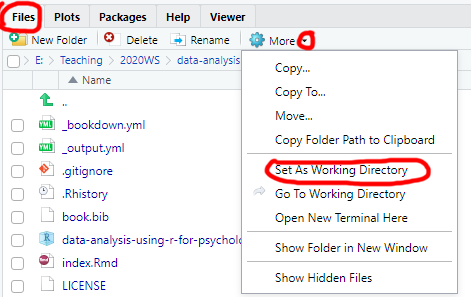
\includegraphics[width=1\linewidth]{images/setwd-gui} \end{center}

In short, you may think that you are working in a particular folder but R will have its own opinion about this. Whenever this happens, it is really confusing and involves a lot of cursing as R cannot find files that you clearly see with your own eyes. To avoid this you should organize any project or seminar as an \emph{R Project}. It assumes that all the necessary files are in the project folder, which is also the working directory. R Studio has some nice project-based touches as well, like keeping tracking of which files you have open, providing version control, etc. Bottom line, \textbf{always} create a new R-project to organize yourself, even if it involves just a single file to try something out. Remember, ``Nothing is more permanent than a temporary solution!'' Which is why you should \textbf{always} write your code, as if it is for a long term project (good style, comprehensible variable names, comments, etc.), otherwise your temporary solution grows into permanent incomprehensible spaghetti code.

Let us create a new project for this seminar. Use \texttt{File\ /\ New\ Project...}, which will give you options of creating it in a new directory (you get to come up with a name), using an existing directory (project will be named after that directory), or check it out from remote repository (something we won't talk about just yet). You can do it either way. This will be the project folder for this seminar and you will need to put all notebooks and external data files into that folder. Next time you need to open it, you can use \texttt{File\ /\ Recent\ Projects} menu, \texttt{File\ /\ Open\ Project...} menu, or simply open the \texttt{\textless{}name-of-your-project\textgreater{}.Rproj} file in that folder.

\hypertarget{rmarkdown}{%
\section{RMarkdown}\label{rmarkdown}}

\href{https://rmarkdown.rstudio.com/}{RMarkdown notebooks} combine formatted text and illustrations with code. When a notebook is ``knitted'', all the code is ran and its output, such as tables and figures, is inserted into the final document. This allows you to combine the narrative (the background, the methodology, discussion, conclusions, etc.) with the actual code that implements what you described.

Importantly, notebooks can be knitted into a variety of formats including HTML, PDF, Word document, EPUB book, etc. Thus, instead of creating plots and tables and saving them into separate files so you can copy-paste them into your Word file (and then redoing it, if something changed, and trying to find the correct code that you used the last time, and wondering why it does not run anymore\ldots), you simply ``knit'' the notebook and get the current and complete research report, semester work, presentation, etc. Even more importantly, same goes for others, as they also can knit your notebook and generate its latest version in format they need. All your exercises will be based on RMarkdown notebooks, so you need to familiarize yourself with them.

We will start by learning the markdown, which is a family of human-oriented markup languages. Markup is a plain text that includes formatting syntax and can be translated into visually formatted text. For example, HTML and LaTeX are markup languages. The advantage of markup is that you do not need a special program to edit it, any plain text editor will suffice. However, you do need a special program to turn this plain text into the document. For example, you need Latex to compile a PDF or a browser to view HTML properly. However, anyone can read your original file even if they do not have Latex, PDF reader, or a browser installed (you do need Word to read a Word file!). \textbf{Markdown} markup language was design to make formatting simple and unobtrusive, so the plain document is easy to read (you can read HTML but it is hardly fun!). It is not as feature-rich as HTML or LaTeX but covers most of your usual needs and is very easy to learn!

Create a new markdown file via \texttt{File\ /\ New\ File\ /\ R\ Markdown...} menu. Use \texttt{Seminar\ 1} for its title and HTML as default output format. Then you need to save the file (pressing \texttt{Ctrl\ +\ S} will suffice) and call the file \texttt{seminar-01} (R Studio will add \texttt{.Rmd} extension automatically). The file you created is not empty, as R Studio is kind enough to provide a template and example for you. Knit the notebook by clicking on \texttt{Knit} button or pressing \texttt{Ctrl\ +\ Shift\ +\ K} to see how the properly typeset text will look (it will appear in \texttt{Viewer} tab).

\begin{center}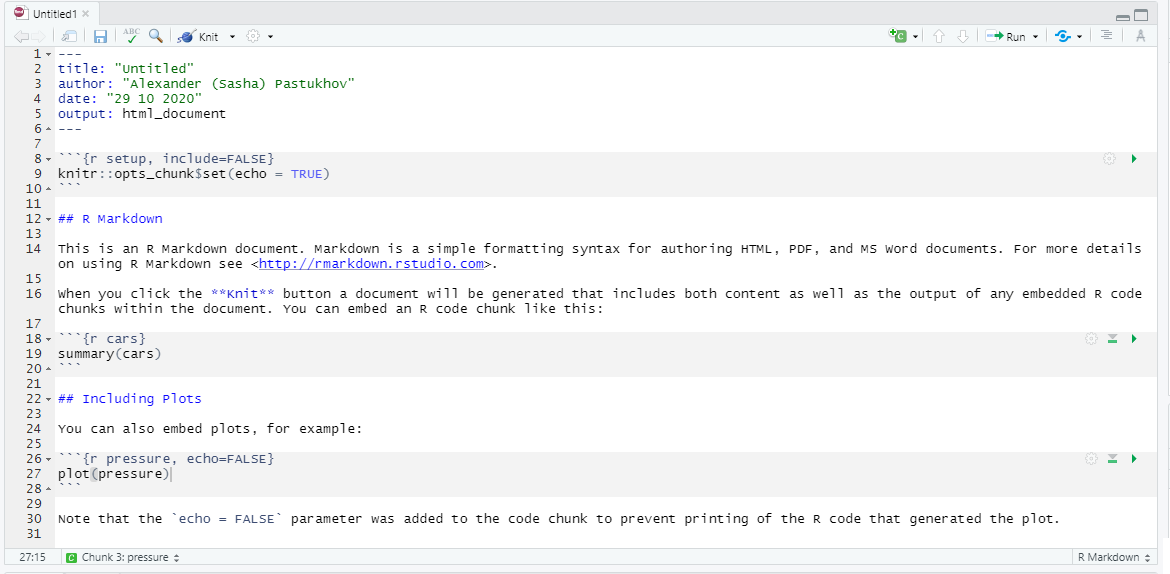
\includegraphics[width=1\linewidth]{images/default-notebook} \end{center}

Let us go through the default notebook that R Studio created for us.

\begin{center}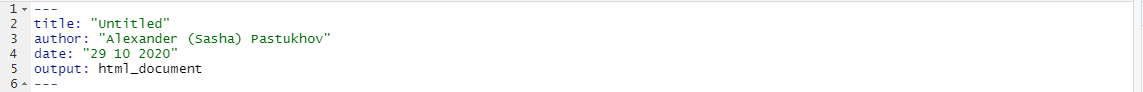
\includegraphics[width=1\linewidth]{images/notebook-header} \end{center}

The top part between two sets of \texttt{-\/-\/-} is a notebook header with various configuration options written in \href{https://yaml.org/}{YAML} (yes, we have two different languages in one file). \texttt{title}, \texttt{author}, and \texttt{date} should be self-explanatory. \texttt{output} defines what kind of output document knitr will generate. You can specify it by hand (e.g., \texttt{word\_document}) or just click on drop down next to \texttt{Knit} button and pick the option you like (we will use the default HTML most of the time). These are sufficient for us but there are numerous other options that you can specify, for example, to enable indexing of headers. You can read about at \href{https://yihui.org/knitr/}{yihui.org/knitr}.

\begin{center}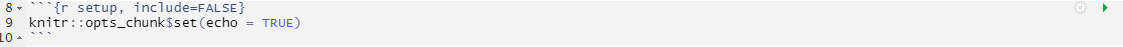
\includegraphics[width=1\linewidth]{images/notebook-setup} \end{center}

The next section is the ``setup code chunk'' that specifies default options on how the code chunks are treated by default (executed or not, their output is shown or not, etc.). By default code in chunks is run and its output is shown (\texttt{echo\ =\ TRUE}) but you can change this behavior on per-chunk basis by pressing the gear button at the top-right. The setup chunk is also a good place to import your libraries (we will talk about it later) as it is always run before any other chunks (so, even if you forgot to run it to load libraries, R Studio will do this for you).

\begin{center}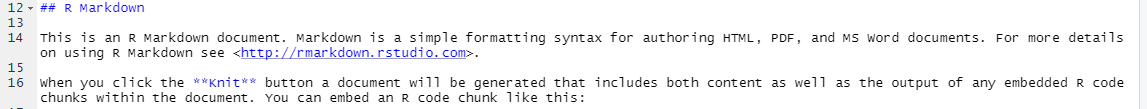
\includegraphics[width=1\linewidth]{images/notebook-text} \end{center}

Next, we have plain text with rmarkdown, which gets translated into formatted text when you click on \texttt{Knit} button. You can write like this anywhere outside of code chunks to explain the logic of your analysis. You should write why and how the analysis is performed but leave technical details on programming to the chunk itself, where you can comment the code.

\begin{center}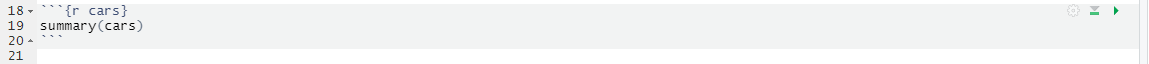
\includegraphics[width=1\linewidth]{images/notebook-chunk} \end{center}

Finally, we have our first ``proper'' chunk of code (the ``setup'' chunk above is a special case). A code chunk is simply the code embedded between
\texttt{\textasciigrave{}\textasciigrave{}\textasciigrave{}\{r\ \textless{}name\ of\ the\ chunk\}} and the seconds set of ticks \texttt{\textasciigrave{}\textasciigrave{}\textasciigrave{}}. Here \texttt{r} specifies that the code inside is written in R language but you can use other languages such as Python, Stan, or SQL. The \texttt{name\ of\ the\ chunk} is optional but I would recommend to have it, as it reminds you what this code is about and it makes it easier to navigate in large notebooks. In the bottom-left corner, you can see which chunk or section you are currently at and, if you click on it, you can quickly navigate to a different chunk. If chunks are not explicitly named, they will get labels \texttt{Chunk\ 1}, \texttt{Chunk\ 2}, etc. making it hard to distinguish them.

\begin{center}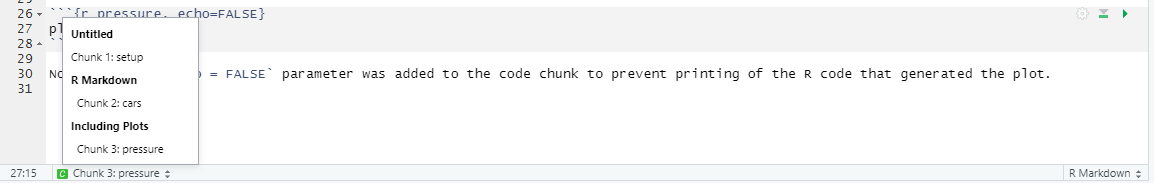
\includegraphics[width=1\linewidth]{images/notebook-navigation} \end{center}

There are also additional options that you can specify per chunk (whether to run the code, to show the output, what size the figures should be, etc.). Generally we won't need these options but you can get an idea about them by looking at the \href{https://yihui.org/knitr/options/}{official manual}. You can create a chunk by hand or click on ``Create chunk'' drop-down list (in this case, it will create the chunk at the position of the cursor)

\begin{center}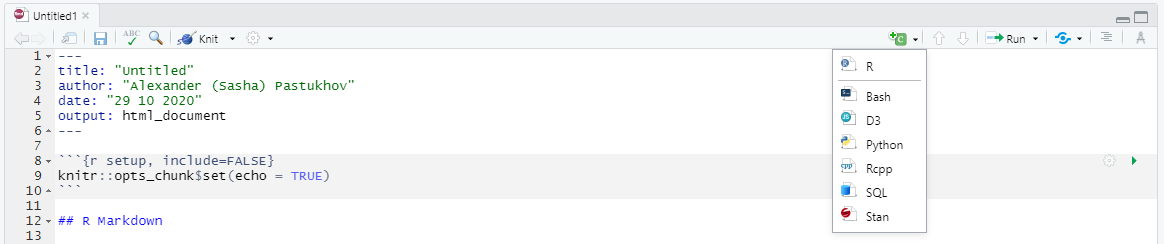
\includegraphics[width=1\linewidth]{images/notebook-insert-chunk} \end{center}

Finally, you run \textbf{all} the code in the chunk by clicking on \texttt{Run\ current\ chunk\ button} at the top-right corner of the chunk or by pressing \texttt{Ctrl\ +\ Shift\ +\ Enter} when the you are inside the chunk. However, you can also run just a \emph{single line} or only \emph{selected lines} by pressing \texttt{Ctrl\ +\ Enter}. The cool thing about RMarkdown in RStudio is that you will see the output of that chunk right below it. This means that you can write you code chunk-by-chunk, ensure that each works as intended and only when knit the entire document. Run the chunks in your notebook to see what I mean.

\begin{center}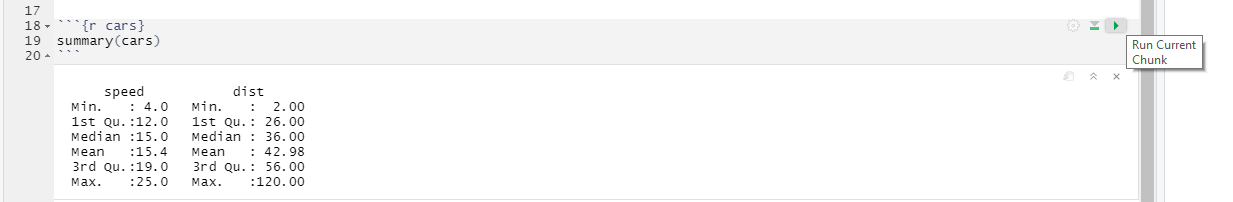
\includegraphics[width=1\linewidth]{images/notebook-run-chunk} \end{center}

\hypertarget{exercise}{%
\section{Exercise}\label{exercise}}

For the today's exercise, I want you to familiarize yourself with markdown. Go to \href{https://www.markdownguide.org/}{markdownguide.org} and look at basic and extended syntax (their cheat sheet is also very good). Write any text you want that uses all the formatting and submit the file to MS Teams.

\hypertarget{vectors}{%
\chapter{Vectors! Vectors everywhere!}\label{vectors}}

Before reading the chapter, please download the \href{notebooks/Seminar\%2002\%20-\%20Vectors.Rmd}{exercise notebook} (\texttt{Alt\ +\ Click} to download it or right-click as \texttt{Save\ link\ as...}), put it into your seminar project folder and open the project. You need both the text and the notebook with exercises to be open, as you will be switching between them.

Before we can start programming in R, you need to learn about vectors. This is a key concept in R, so your understanding of it will determine how easy it will be for you to use R. Do all of the exercises and do not hesitate to ask me whenever something is unclear. Remember, you need to master vectors before you can master R!

\hypertarget{variables}{%
\section{Variables as boxes}\label{variables}}

In programming, the concept of a variable is often described as a box you can put something in. A box has a name tag on it, which is the \emph{name} of the variable. Whatever you put in is the \emph{value} that you store.

\begin{center}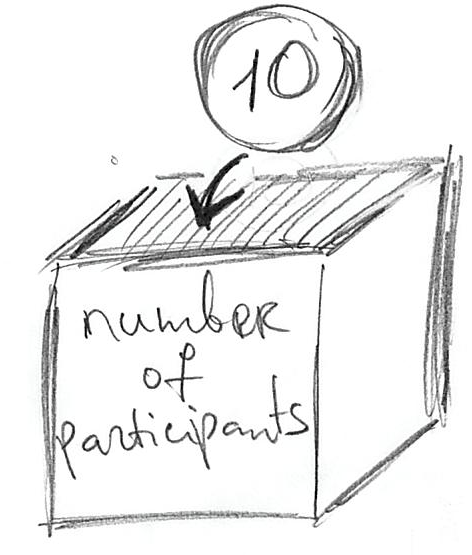
\includegraphics[width=0.3\linewidth]{images/variable-as-box} \end{center}

This ``putting in'' concepts is reflected in R syntax

\begin{Shaded}
\begin{Highlighting}[]
\NormalTok{number\_of\_participants }\OtherTok{\textless{}{-}} \DecValTok{10}
\end{Highlighting}
\end{Shaded}

Here, \texttt{number\_of\_participants} is the name of the variable (name tag for the box we will be using), \texttt{10} is the value you store, and \texttt{\textless{}-} means \textbf{``put \texttt{10} into variable \texttt{number\_of\_participants}''}. If you know other programming languages, you probably expected the usual assignment operator \texttt{=}. Confusingly, you can use it as well, but there are some subtle, yet important, differences in how they operate behind the scenes. We will meet \texttt{=} again when we will be talking about functions and, in particular, Tidyverse way of doing things but for now \textbf{only use \texttt{\textless{}-} operator}!

\hypertarget{assignment-statement-in-detail}{%
\section{Assignment statement in detail}\label{assignment-statement-in-detail}}

One \textbf{very important} thing to remember about the assignment statement \texttt{\textless{}variable\textgreater{}\ \textless{}-\ \textless{}value\textgreater{}}: the \emph{right side} is evaluated first until the final value is established and then, and only then, it is stored in a \texttt{\textless{}variable\textgreater{}} specified on the left side. This means that you can use the same variable on \emph{both} sides. Take a look at the example

\begin{Shaded}
\begin{Highlighting}[]
\NormalTok{x }\OtherTok{\textless{}{-}} \DecValTok{2}
\FunctionTok{print}\NormalTok{(x)}
\end{Highlighting}
\end{Shaded}

\begin{verbatim}
## [1] 2
\end{verbatim}

\begin{Shaded}
\begin{Highlighting}[]
\NormalTok{x }\OtherTok{\textless{}{-}}\NormalTok{ x }\SpecialCharTok{+} \DecValTok{5}
\FunctionTok{print}\NormalTok{(x)}
\end{Highlighting}
\end{Shaded}

\begin{verbatim}
## [1] 7
\end{verbatim}

We are storing value \texttt{2} in a variable \texttt{x}. In the next line, the \emph{right side} is evaluated first. This means that the current value of \texttt{x} is substituted in its place on the right side: \texttt{x\ +\ 5} becomes \texttt{2\ +\ 5}. This expression computed and we get \texttt{7}. Now, that the \emph{right side} is fully evaluated, the value can be stored in \texttt{x} replacing (overwriting) the original value it had.

R's use of \texttt{\textless{}-} makes it easier to memorize this \emph{right side is fully evaluated first} rule. However, as noted above, we will meet \texttt{=} operator and this one makes it look like a mathematical equation. However, assignments (storing values in a variable) have nothing in common with mathematical equations (finding values of variables to ensure equality)!

Do exercise 1.

\hypertarget{vectors-scalars}{%
\section{Vectors and scalars (which are also vectors)}\label{vectors-scalars}}

The box metaphor you've just learned, doesn't quite work for R. Historically, R was developed as a language for statistical computing, so it was based on concepts of linear algebra instead of being a ``normal'' programming language. This means that there is no conceptual divide between single values and containers (arrays, lists, dictionaries, etc.) that hold many single values. Instead, the primary data unit in R is a \textbf{vector}, which you may remember from geometry or, hopefully, from linear algebra, as an arrow that goes from 0 to a specific point in space. From computer science point of view, a vector is just a list of numbers (or some other values, as you will learn later). This means that there are no ``single values'' in R, there are only vectors of variable length. Special cases are vectors of length one, which are called \emph{scalars} \footnote{Multiplication of a vector by another vector \emph{transforms} it but for a single element vector the only transformation you can get is ``scaling'', hence, the name.} (but they are still vectors) and zero length vectors that are, sort of, a Platonic idea of a vector without actual values. With respect to the ``box metaphor'', this means that we always have a box with indexed (numbered) slots in it. A simple assignment makes sure that ``the box'' has as many slots as the values you want to put in and stores these values one after another starting with slot \#1. So, the example above \texttt{number\_of\_participants\ \textless{}-\ 10} creates a variable with one (1) slot and stores the value in it.

\begin{center}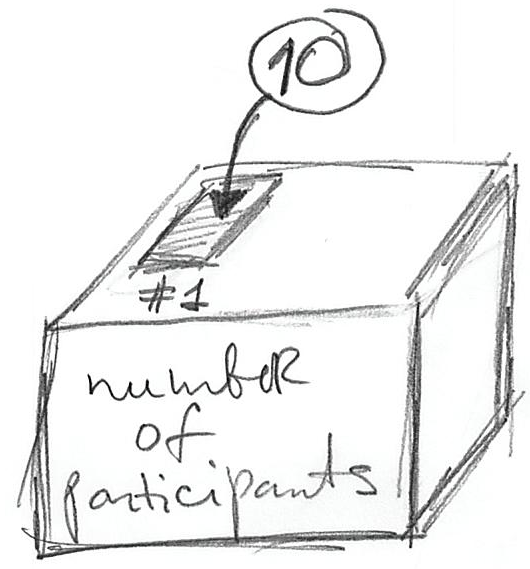
\includegraphics[width=0.3\linewidth]{images/box-with-a-slot} \end{center}

But, as noted above, a single value (vector with length of one) is a special case. More generally you write:

\begin{Shaded}
\begin{Highlighting}[]
\NormalTok{response }\OtherTok{\textless{}{-}} \FunctionTok{c}\NormalTok{(}\DecValTok{1}\NormalTok{, }\DecValTok{7}\NormalTok{, }\DecValTok{3}\NormalTok{)}
\end{Highlighting}
\end{Shaded}

Here, you create a variable (box) named \texttt{response} that has three slots in it because you want to store three values. You put values \texttt{1}, \texttt{7}, \texttt{3} into the slots \#1, \#2, and \#3. The \texttt{c(1,\ 7,\ 3)} notation is how you create a vector in R by \href{https://www.rdocumentation.org/packages/base/versions/3.6.2/topics/c}{\textbf{c}oncatenating} (or \textbf{c}ombining) values\footnote{I find this to be a poor choice of name but we are stuck with, so get used to it.}. The figure below illustrates the idea:

\begin{center}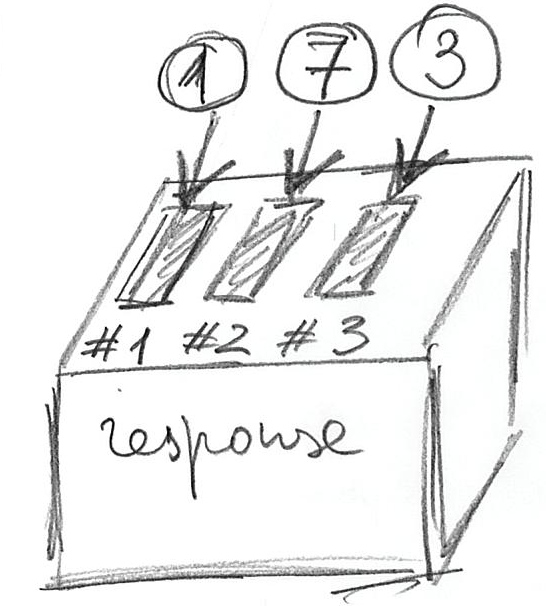
\includegraphics[width=0.3\linewidth]{images/box-3-slots} \end{center}

Building on the box metaphor: If you can store something in a box, you can take it out! In the world of computers it works even better, because rather than taking something out, you just make a copy of that and store this copy somewhere else or to use it to compute things. Minimally, we would like to see what is inside of the box. For this, you can use \href{https://www.rdocumentation.org/packages/base/versions/3.6.2/topics/print}{print} function:

\begin{Shaded}
\begin{Highlighting}[]
\NormalTok{response }\OtherTok{\textless{}{-}} \FunctionTok{c}\NormalTok{(}\DecValTok{1}\NormalTok{, }\DecValTok{7}\NormalTok{, }\DecValTok{3}\NormalTok{)}
\FunctionTok{print}\NormalTok{(response)}
\end{Highlighting}
\end{Shaded}

\begin{verbatim}
## [1] 1 7 3
\end{verbatim}

Or, we can make a copy of values in one variable and store them in another:

\begin{Shaded}
\begin{Highlighting}[]
\NormalTok{x }\OtherTok{\textless{}{-}} \FunctionTok{c}\NormalTok{(}\DecValTok{3}\NormalTok{, }\DecValTok{6}\NormalTok{, }\DecValTok{9}\NormalTok{)}
\NormalTok{y }\OtherTok{\textless{}{-}}\NormalTok{ x }

\FunctionTok{print}\NormalTok{(x)}
\end{Highlighting}
\end{Shaded}

\begin{verbatim}
## [1] 3 6 9
\end{verbatim}

\begin{Shaded}
\begin{Highlighting}[]
\FunctionTok{print}\NormalTok{(y)}
\end{Highlighting}
\end{Shaded}

\begin{verbatim}
## [1] 3 6 9
\end{verbatim}

Here, we create a 3-slot variable \texttt{x} so that we can put in a vector of length 3 created via concatenation \texttt{c(3,\ 6,\ 9)}. Next, we make a copy of these three values and store them in a different variable \texttt{y}. Importantly, the values in variable \texttt{x} stayed as they were. Take a look at the figure below, which graphically illustrate this:

\begin{center}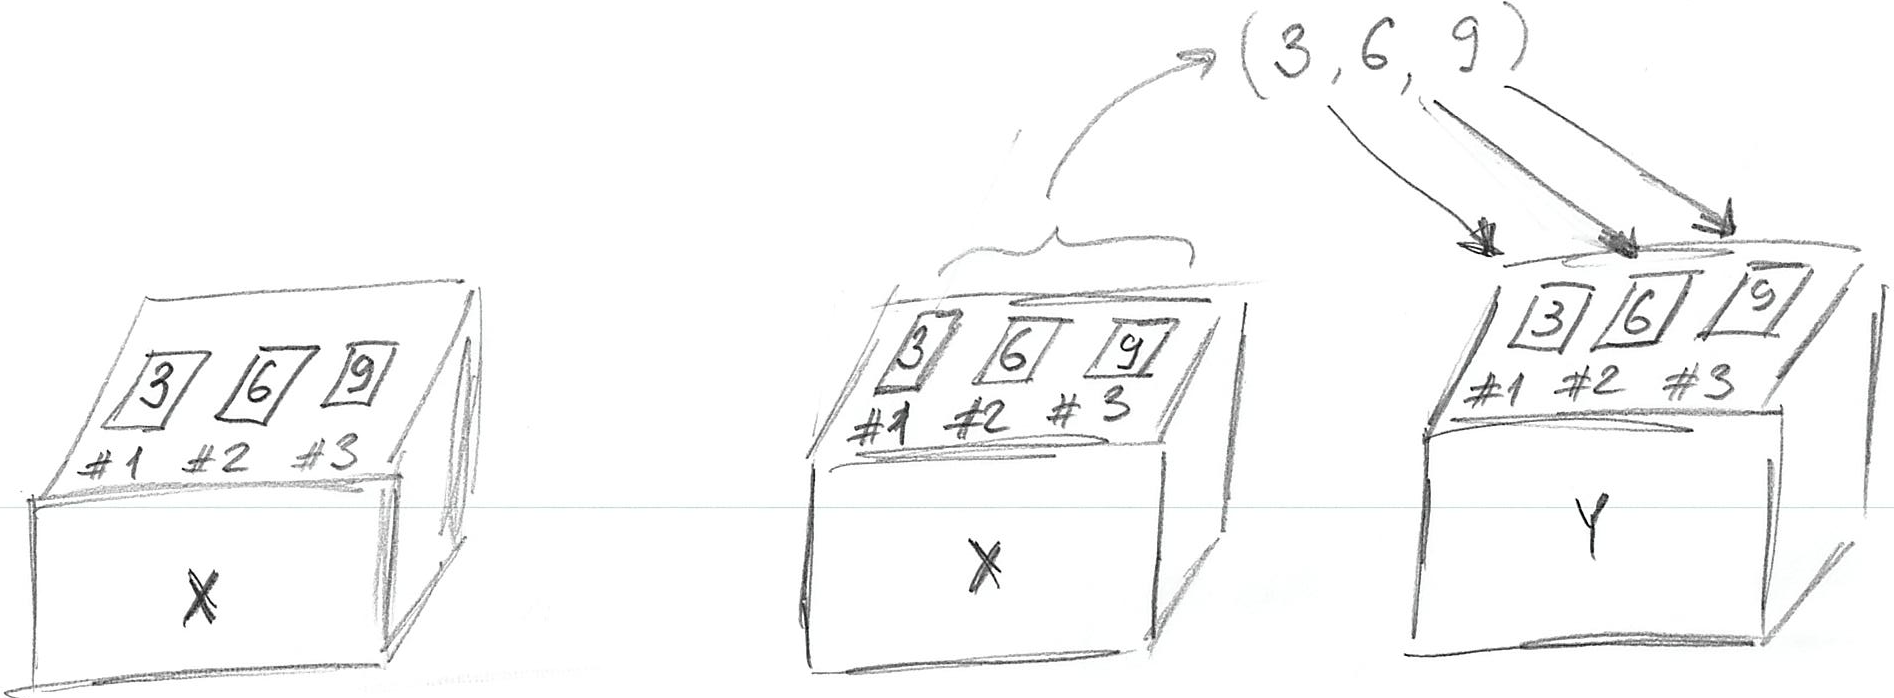
\includegraphics[width=1\linewidth]{images/copy-vector} \end{center}

Do exercise 2.

Remember, everything is a vector! This means that \texttt{c(3,\ 6,\ 9)} does not \textbf{c}oncatenate numbers, it \textbf{c}oncatenates three length one vectors (scalars) \texttt{3}, \texttt{6}, \texttt{9}. Thus, \textbf{c}oncatenation works on longer vectors in exactly the same way:

\begin{Shaded}
\begin{Highlighting}[]
\NormalTok{x }\OtherTok{\textless{}{-}} \FunctionTok{c}\NormalTok{(}\DecValTok{1}\NormalTok{, }\DecValTok{2}\NormalTok{, }\DecValTok{3}\NormalTok{)}
\NormalTok{y }\OtherTok{\textless{}{-}} \FunctionTok{c}\NormalTok{(}\DecValTok{4}\NormalTok{, }\DecValTok{5}\NormalTok{)}
\FunctionTok{print}\NormalTok{(}\FunctionTok{c}\NormalTok{(x, y))}
\end{Highlighting}
\end{Shaded}

\begin{verbatim}
## [1] 1 2 3 4 5
\end{verbatim}

Do exercise 3.

\hypertarget{vector-index}{%
\section{Vector indexes}\label{vector-index}}

A vector is an ordered list of one or more values (box with one or more slots) and, sometimes, you need only one of the values. Each value (slot in the box) has its own index from 1 till N, where N is the \href{https://www.rdocumentation.org/packages/base/versions/3.6.2/topics/length}{length} of the vector. To access that slot you use square brackets \texttt{some\_vector{[}index{]}}. You can both get and set the value for the individual slots the same way you do it for the whole vector.

\begin{Shaded}
\begin{Highlighting}[]
\NormalTok{x }\OtherTok{\textless{}{-}} \FunctionTok{c}\NormalTok{(}\DecValTok{1}\NormalTok{, }\DecValTok{2}\NormalTok{, }\DecValTok{3}\NormalTok{)}
\CommentTok{\# set SECOND element to 4}
\NormalTok{x[}\DecValTok{2}\NormalTok{] }\OtherTok{\textless{}{-}} \DecValTok{4}

\CommentTok{\# print the entire vector}
\FunctionTok{print}\NormalTok{(x)}
\end{Highlighting}
\end{Shaded}

\begin{verbatim}
## [1] 1 4 3
\end{verbatim}

\begin{Shaded}
\begin{Highlighting}[]
\CommentTok{\# print only the third element}
\FunctionTok{print}\NormalTok{(x[}\DecValTok{3}\NormalTok{])}
\end{Highlighting}
\end{Shaded}

\begin{verbatim}
## [1] 3
\end{verbatim}

Do exercise 4.

Unfortunately, vector indexing in R behaves in a way that may catch you by surprise. If your vectors contains five values, you would expect that index of \texttt{0} (negative indexes are discussed below) or above \texttt{5} generates an error. Not in R! Index of \texttt{0} is a special case and produces an \emph{empty vector} (vector of zero length).

\begin{Shaded}
\begin{Highlighting}[]
\NormalTok{x }\OtherTok{\textless{}{-}} \FunctionTok{c}\NormalTok{(}\DecValTok{1}\NormalTok{, }\DecValTok{2}\NormalTok{, }\DecValTok{3}\NormalTok{)}
\NormalTok{x[}\DecValTok{0}\NormalTok{]}
\end{Highlighting}
\end{Shaded}

\begin{verbatim}
## numeric(0)
\end{verbatim}

If you try to get vector element using index that is larger than vector length (so \texttt{6} and above, if your vector length is 5), R will return \texttt{NA} (``Not Available'' / Missing Value).

\begin{Shaded}
\begin{Highlighting}[]
\NormalTok{x }\OtherTok{\textless{}{-}} \FunctionTok{c}\NormalTok{(}\DecValTok{1}\NormalTok{, }\DecValTok{2}\NormalTok{, }\DecValTok{3}\NormalTok{)}
\NormalTok{x[}\DecValTok{5}\NormalTok{]}
\end{Highlighting}
\end{Shaded}

\begin{verbatim}
## [1] NA
\end{verbatim}

In both cases, it won't generate an error or even warn you!

When \textbf{setting} the value by index, using \texttt{0} will produce no effect, because you are trying to put a value in a vector with no slots. Oddly enough, this will generate neither an error nor a warning, so beware!

\begin{Shaded}
\begin{Highlighting}[]
\NormalTok{x }\OtherTok{\textless{}{-}} \FunctionTok{c}\NormalTok{(}\DecValTok{1}\NormalTok{, }\DecValTok{2}\NormalTok{, }\DecValTok{3}\NormalTok{)}
\NormalTok{x[}\DecValTok{0}\NormalTok{] }\OtherTok{\textless{}{-}} \DecValTok{5}
\FunctionTok{print}\NormalTok{(x)}
\end{Highlighting}
\end{Shaded}

\begin{verbatim}
## [1] 1 2 3
\end{verbatim}

If you set an element those index is \textbf{larger} than vector length, the vector will be automatically expanded to that length and all the elements between the old values and the new one will be \texttt{NA} (Missing Value / Not Available).

\begin{Shaded}
\begin{Highlighting}[]
\NormalTok{x }\OtherTok{\textless{}{-}} \FunctionTok{c}\NormalTok{(}\DecValTok{1}\NormalTok{, }\DecValTok{2}\NormalTok{, }\DecValTok{3}\NormalTok{)}
\NormalTok{x[}\DecValTok{10}\NormalTok{] }\OtherTok{\textless{}{-}} \DecValTok{5}
\FunctionTok{print}\NormalTok{(x)}
\end{Highlighting}
\end{Shaded}

\begin{verbatim}
##  [1]  1  2  3 NA NA NA NA NA NA  5
\end{verbatim}

This may sound too technical but I want you to learn about this because R conventions are so different from other programming languages and, also, from you would intuitively expect. If you are not aware of these highly peculiar rules, you may never realize that your code is not working properly because you will never see an error or even a warning! It should also make you more cautious and careful when programming in R. It is a very powerful language that allows you to be very flexible and expressive. Unfortunately, that flexibility means that base R won't stop you from shooting yourself in a foot. Even worse, sometimes you won't even notice that your foot is shot because R won't generate either errors or warnings, as in examples above. Good news is that things are far more restricted and consistent in Tidyverse.

Do exercise 5.

Also, you can use \emph{negative} indexes. In that case, you \textbf{exclude} the value with that index and return or modify the rest.

\begin{Shaded}
\begin{Highlighting}[]
\NormalTok{x }\OtherTok{\textless{}{-}} \FunctionTok{c}\NormalTok{(}\DecValTok{1}\NormalTok{, }\DecValTok{2}\NormalTok{, }\DecValTok{3}\NormalTok{, }\DecValTok{4}\NormalTok{, }\DecValTok{5}\NormalTok{)}
\CommentTok{\# this will return all elements but \#3}
\NormalTok{x[}\SpecialCharTok{{-}}\DecValTok{3}\NormalTok{] }
\end{Highlighting}
\end{Shaded}

\begin{verbatim}
## [1] 1 2 4 5
\end{verbatim}

\begin{Shaded}
\begin{Highlighting}[]
\NormalTok{x }\OtherTok{\textless{}{-}} \FunctionTok{c}\NormalTok{(}\DecValTok{1}\NormalTok{, }\DecValTok{2}\NormalTok{, }\DecValTok{3}\NormalTok{, }\DecValTok{4}\NormalTok{, }\DecValTok{5}\NormalTok{)}
\CommentTok{\# this will assign new value (by repeating length one vector) to all elements but \#2}
\NormalTok{x[}\SpecialCharTok{{-}}\DecValTok{2}\NormalTok{] }\OtherTok{\textless{}{-}} \DecValTok{10}
\NormalTok{x}
\end{Highlighting}
\end{Shaded}

\begin{verbatim}
## [1] 10  2 10 10 10
\end{verbatim}

Given that negative indexing returns everything \textbf{but} the indexed value, what do you think will happen here?

\begin{Shaded}
\begin{Highlighting}[]
\NormalTok{x }\OtherTok{\textless{}{-}} \FunctionTok{c}\NormalTok{(}\DecValTok{10}\NormalTok{, }\DecValTok{20}\NormalTok{, }\DecValTok{30}\NormalTok{, }\DecValTok{40}\NormalTok{, }\DecValTok{50}\NormalTok{)}
\NormalTok{x[}\SpecialCharTok{{-}}\DecValTok{10}\NormalTok{]}
\end{Highlighting}
\end{Shaded}

Do exercise 6.

Finally, somewhat illogically, the entire vector is returned if you do not specify the index in the square brackets. Here, lack of index means ``everything''.

\begin{Shaded}
\begin{Highlighting}[]
\NormalTok{x }\OtherTok{\textless{}{-}} \FunctionTok{c}\NormalTok{(}\DecValTok{10}\NormalTok{, }\DecValTok{20}\NormalTok{, }\DecValTok{30}\NormalTok{, }\DecValTok{40}\NormalTok{, }\DecValTok{50}\NormalTok{)}
\NormalTok{x[]}
\end{Highlighting}
\end{Shaded}

\begin{verbatim}
## [1] 10 20 30 40 50
\end{verbatim}

\hypertarget{names-as-index}{%
\section{Names as Index}\label{names-as-index}}

As you've just learned, every slot in vector has its numeric (integer) index. However, this number only indicates an index of a slot but tells you nothing on how it is conceptually different from a slot with a different index. For example, if we are storing width and height in a vector, remembering their order may be tricky: was it \texttt{box\_size\ \textless{}-\ c(\textless{}width\textgreater{},\ \textless{}depth\textgreater{},\ \textless{}height\textgreater{})} or \texttt{box\_size\ \textless{}-\ c(\textless{}height\textgreater{},\ \textless{}width\textgreater{},\ \textless{}depth\textgreater{})}? Similarly, looking at \texttt{box\_size{[}1{]}} tells that you are definitely using the \emph{first} dimension but is it \texttt{height} or \texttt{width} (or \texttt{depth})?

In R, you can use \emph{names} to supplement numeric indexes. It allows you add meaning to a particular vector index, something that becomes extremely important when we use it for tables. There are two ways to assign names to indexes, either when you are creating the index via \texttt{c()} function or, afterwards, via \href{https://www.rdocumentation.org/packages/base/versions/3.6.2/topics/names}{names()} function.

To create named vector via \texttt{c()} you specify a name before each value as \texttt{c(\textless{}name1\textgreater{}\ =\ \textless{}value1\textgreater{},\ \textless{}name2\textgreater{}\ =\ \textless{}value2\textgreater{},\ ...)}:

\begin{Shaded}
\begin{Highlighting}[]
\NormalTok{box\_size }\OtherTok{\textless{}{-}} \FunctionTok{c}\NormalTok{(}\StringTok{"width"}\OtherTok{=}\DecValTok{2}\NormalTok{, }\StringTok{"height"}\OtherTok{=}\DecValTok{4}\NormalTok{, }\StringTok{"depth"}\OtherTok{=}\DecValTok{1}\NormalTok{) }
\FunctionTok{print}\NormalTok{(box\_size)}
\end{Highlighting}
\end{Shaded}

\begin{verbatim}
##  width height  depth 
##      2      4      1
\end{verbatim}

Note the names appearing above each value. You can now use either numeric index or name to access the value.

\begin{Shaded}
\begin{Highlighting}[]
\NormalTok{box\_size }\OtherTok{\textless{}{-}} \FunctionTok{c}\NormalTok{(}\StringTok{"width"}\OtherTok{=}\DecValTok{2}\NormalTok{, }\StringTok{"height"}\OtherTok{=}\DecValTok{4}\NormalTok{, }\StringTok{"depth"}\OtherTok{=}\DecValTok{1}\NormalTok{) }
\FunctionTok{print}\NormalTok{(box\_size[}\DecValTok{1}\NormalTok{])}
\end{Highlighting}
\end{Shaded}

\begin{verbatim}
## width 
##     2
\end{verbatim}

\begin{Shaded}
\begin{Highlighting}[]
\FunctionTok{print}\NormalTok{(box\_size[}\StringTok{"depth"}\NormalTok{])}
\end{Highlighting}
\end{Shaded}

\begin{verbatim}
## depth 
##     1
\end{verbatim}

Alternatively, you can use \href{https://www.rdocumentation.org/packages/base/versions/3.6.2/topics/names}{names()} function to both get and set the names. The latter works via a \emph{very counterintuitive} syntax \texttt{names(\textless{}vector\textgreater{})\ \textless{}-\ \textless{}vector-with-names\textgreater{}}

\begin{Shaded}
\begin{Highlighting}[]
\CommentTok{\# without names}
\NormalTok{box\_size }\OtherTok{\textless{}{-}} \FunctionTok{c}\NormalTok{(}\DecValTok{2}\NormalTok{, }\DecValTok{4}\NormalTok{, }\DecValTok{1}\NormalTok{) }
\FunctionTok{print}\NormalTok{(box\_size)}
\end{Highlighting}
\end{Shaded}

\begin{verbatim}
## [1] 2 4 1
\end{verbatim}

\begin{Shaded}
\begin{Highlighting}[]
\CommentTok{\# with names}
\FunctionTok{names}\NormalTok{(box\_size) }\OtherTok{\textless{}{-}} \FunctionTok{c}\NormalTok{(}\StringTok{"width"}\NormalTok{, }\StringTok{"height"}\NormalTok{, }\StringTok{"depth"}\NormalTok{)}
\FunctionTok{print}\NormalTok{(box\_size)}
\end{Highlighting}
\end{Shaded}

\begin{verbatim}
##  width height  depth 
##      2      4      1
\end{verbatim}

\begin{Shaded}
\begin{Highlighting}[]
\CommentTok{\# getting all the names}
\FunctionTok{print}\NormalTok{(}\FunctionTok{names}\NormalTok{(box\_size))}
\end{Highlighting}
\end{Shaded}

\begin{verbatim}
## [1] "width"  "height" "depth"
\end{verbatim}

Because everything is a vector, \texttt{names(\textless{}vector\textgreater{})} is also a vector, meaning that you can get or set just one element of it.

\begin{Shaded}
\begin{Highlighting}[]
\NormalTok{box\_size }\OtherTok{\textless{}{-}} \FunctionTok{c}\NormalTok{(}\StringTok{"width"}\OtherTok{=}\DecValTok{2}\NormalTok{, }\StringTok{"height"}\OtherTok{=}\DecValTok{4}\NormalTok{, }\StringTok{"depth"}\OtherTok{=}\DecValTok{1}\NormalTok{) }

\CommentTok{\# modify SECOND name}
\FunctionTok{names}\NormalTok{(box\_size)[}\DecValTok{2}\NormalTok{] }\OtherTok{\textless{}{-}} \StringTok{"HEIGHT"}
\FunctionTok{print}\NormalTok{(box\_size)}
\end{Highlighting}
\end{Shaded}

\begin{verbatim}
##  width HEIGHT  depth 
##      2      4      1
\end{verbatim}

Finally, if you use a name that is not in the index, this is like using numeric index larger than the vector length. Is in out-of-range numeric index, there will be neither error not warning and you will get an \texttt{NA} back.

\begin{Shaded}
\begin{Highlighting}[]
\NormalTok{box\_size }\OtherTok{\textless{}{-}} \FunctionTok{c}\NormalTok{(}\StringTok{"width"}\OtherTok{=}\DecValTok{2}\NormalTok{, }\StringTok{"height"}\OtherTok{=}\DecValTok{4}\NormalTok{, }\StringTok{"depth"}\OtherTok{=}\DecValTok{1}\NormalTok{) }
\FunctionTok{print}\NormalTok{(box\_size[}\StringTok{"radius"}\NormalTok{])}
\end{Highlighting}
\end{Shaded}

\begin{verbatim}
## <NA> 
##   NA
\end{verbatim}

Do exercise 7.

\hypertarget{vector-index-slicing}{%
\section{Slicing}\label{vector-index-slicing}}

So far we were reading or modifying either the whole vector or just one of its elements. However, the index you pass in square brackets (you've guess it!) is also a vector! Which means that you can construct a vector of indexes the same way you construct a vector of any values (the only restriction is that index values must integers and that you cannot mix negative and positive indexes).

\begin{Shaded}
\begin{Highlighting}[]
\NormalTok{x }\OtherTok{\textless{}{-}} \FunctionTok{c}\NormalTok{(}\DecValTok{10}\NormalTok{, }\DecValTok{20}\NormalTok{, }\DecValTok{30}\NormalTok{, }\DecValTok{40}\NormalTok{, }\DecValTok{50}\NormalTok{)}
\NormalTok{x[}\FunctionTok{c}\NormalTok{(}\DecValTok{2}\NormalTok{, }\DecValTok{3}\NormalTok{, }\DecValTok{5}\NormalTok{)]}
\end{Highlighting}
\end{Shaded}

\begin{verbatim}
## [1] 20 30 50
\end{verbatim}

When constructing a vector index, you can put the index values in the order you require (starting from the end of it, random order, etc.) or use the same index more than once.

\begin{Shaded}
\begin{Highlighting}[]
\NormalTok{x }\OtherTok{\textless{}{-}} \FunctionTok{c}\NormalTok{(}\DecValTok{10}\NormalTok{, }\DecValTok{20}\NormalTok{, }\DecValTok{30}\NormalTok{, }\DecValTok{40}\NormalTok{, }\DecValTok{50}\NormalTok{)}
\NormalTok{x[}\FunctionTok{c}\NormalTok{(}\DecValTok{3}\NormalTok{, }\DecValTok{5}\NormalTok{, }\DecValTok{1}\NormalTok{, }\DecValTok{1}\NormalTok{, }\DecValTok{4}\NormalTok{)]}
\end{Highlighting}
\end{Shaded}

\begin{verbatim}
## [1] 30 50 10 10 40
\end{verbatim}

You can also use several negative indexes to exclude multiple values and return the rest. Here, neither order nor the duplicate indexes matter. Regardless of which value you exclude first or how many times you exclude it, you still get \emph{the rest} of the vector in its default order.

\begin{Shaded}
\begin{Highlighting}[]
\NormalTok{x }\OtherTok{\textless{}{-}} \FunctionTok{c}\NormalTok{(}\DecValTok{10}\NormalTok{, }\DecValTok{20}\NormalTok{, }\DecValTok{30}\NormalTok{, }\DecValTok{40}\NormalTok{, }\DecValTok{50}\NormalTok{)}
\NormalTok{x[}\FunctionTok{c}\NormalTok{(}\SpecialCharTok{{-}}\DecValTok{4}\NormalTok{, }\SpecialCharTok{{-}}\DecValTok{2}\NormalTok{, }\SpecialCharTok{{-}}\DecValTok{2}\NormalTok{)]}
\end{Highlighting}
\end{Shaded}

\begin{verbatim}
## [1] 10 30 50
\end{verbatim}

Note that you cannot mix positive and negative indexes as R will generate an error (at last!).

\begin{Shaded}
\begin{Highlighting}[]
\NormalTok{x }\OtherTok{\textless{}{-}} \FunctionTok{c}\NormalTok{(}\DecValTok{10}\NormalTok{, }\DecValTok{20}\NormalTok{, }\DecValTok{30}\NormalTok{, }\DecValTok{40}\NormalTok{, }\DecValTok{50}\NormalTok{)}

\CommentTok{\# THIS WILL GENERATE AN ERROR: }
\CommentTok{\# "Error in x[c({-}4, 2, {-}2)] : only 0\textquotesingle{}s may be mixed with negative subscripts"}
\NormalTok{x[}\FunctionTok{c}\NormalTok{(}\SpecialCharTok{{-}}\DecValTok{4}\NormalTok{, }\DecValTok{2}\NormalTok{, }\SpecialCharTok{{-}}\DecValTok{2}\NormalTok{)]}
\end{Highlighting}
\end{Shaded}

Finally, including zero index makes no difference but generates neither an error nor a warning.

\begin{Shaded}
\begin{Highlighting}[]
\NormalTok{x }\OtherTok{\textless{}{-}} \FunctionTok{c}\NormalTok{(}\DecValTok{10}\NormalTok{, }\DecValTok{20}\NormalTok{, }\DecValTok{30}\NormalTok{, }\DecValTok{40}\NormalTok{, }\DecValTok{50}\NormalTok{)}
\NormalTok{x[}\FunctionTok{c}\NormalTok{(}\DecValTok{1}\NormalTok{, }\DecValTok{0}\NormalTok{, }\DecValTok{5}\NormalTok{, }\DecValTok{0}\NormalTok{, }\DecValTok{0}\NormalTok{, }\DecValTok{2}\NormalTok{, }\DecValTok{2}\NormalTok{)]}
\end{Highlighting}
\end{Shaded}

\begin{verbatim}
## [1] 10 50 20 20
\end{verbatim}

You can also use names instead of numeric indexes.

\begin{Shaded}
\begin{Highlighting}[]
\NormalTok{box\_size }\OtherTok{\textless{}{-}} \FunctionTok{c}\NormalTok{(}\StringTok{"width"}\OtherTok{=}\DecValTok{2}\NormalTok{, }\StringTok{"height"}\OtherTok{=}\DecValTok{4}\NormalTok{, }\StringTok{"depth"}\OtherTok{=}\DecValTok{1}\NormalTok{) }
\FunctionTok{print}\NormalTok{(box\_size[}\FunctionTok{c}\NormalTok{(}\StringTok{"height"}\NormalTok{, }\StringTok{"width"}\NormalTok{)])}
\end{Highlighting}
\end{Shaded}

\begin{verbatim}
## height  width 
##      4      2
\end{verbatim}

However, you cannot mix numeric indexes and names. The reason is that a vector can hold only values of one type (more on that during the next seminar), so all numeric values will be converted to text (\texttt{1} will become \texttt{"1"}) and treated as names rather than indexes.

\hypertarget{colon-sequence}{%
\section{Colon Operator and Sequence Generation}\label{colon-sequence}}

To simplify vector indexing, R provides you with a shortcut to create a range of values. An expression \texttt{A:B} (a.k.a.\href{https://stat.ethz.ch/R-manual/R-devel/library/base/html/Colon.html}{Colon Operator}) builds a sequence of integers starting with \texttt{A} and ending with \textbf{and including(!)} \texttt{B} (the latter is not so obvious, if you come from Python).

\begin{Shaded}
\begin{Highlighting}[]
\DecValTok{3}\SpecialCharTok{:}\DecValTok{7}
\end{Highlighting}
\end{Shaded}

\begin{verbatim}
## [1] 3 4 5 6 7
\end{verbatim}

Thus, you can use it to easily create an index and, because everything is a vector!, combine it with other values.

\begin{Shaded}
\begin{Highlighting}[]
\NormalTok{x }\OtherTok{\textless{}{-}} \FunctionTok{c}\NormalTok{(}\DecValTok{10}\NormalTok{, }\DecValTok{20}\NormalTok{, }\DecValTok{30}\NormalTok{, }\DecValTok{40}\NormalTok{, }\DecValTok{50}\NormalTok{)}
\NormalTok{x[}\FunctionTok{c}\NormalTok{(}\DecValTok{1}\NormalTok{, }\DecValTok{3}\SpecialCharTok{:}\DecValTok{5}\NormalTok{)]}
\end{Highlighting}
\end{Shaded}

\begin{verbatim}
## [1] 10 30 40 50
\end{verbatim}

The sequence above is increasing but you can also use the colon operator to construct a decreasing one.

\begin{Shaded}
\begin{Highlighting}[]
\NormalTok{x }\OtherTok{\textless{}{-}} \FunctionTok{c}\NormalTok{(}\DecValTok{10}\NormalTok{, }\DecValTok{20}\NormalTok{, }\DecValTok{30}\NormalTok{, }\DecValTok{40}\NormalTok{, }\DecValTok{50}\NormalTok{)}
\NormalTok{x[}\FunctionTok{c}\NormalTok{(}\DecValTok{5}\SpecialCharTok{:}\DecValTok{2}\NormalTok{)]}
\end{Highlighting}
\end{Shaded}

\begin{verbatim}
## [1] 50 40 30 20
\end{verbatim}

The colon operator is limited to sequences with steps of \texttt{1} (if end value is larger than the start value) or \texttt{-1} (if end value is smaller than the start value). For more flexibility you can use \href{https://stat.ethz.ch/R-manual/R-devel/library/base/html/seq.html}{Sequence Generation} function: \texttt{seq(from,\ to,\ by,\ length.out)}. The \texttt{from} and \texttt{to} are starting and ending values (just like in the colon operator) and you can specify either a step via \texttt{by} parameter (as, in ``from A to B by C'') or via \texttt{length.out} parameter (how many values you want to generate, effectively \texttt{by\ =\ ((to\ -\ from)/(length.out\ -\ 1)}).
Using \texttt{by} version:

\begin{Shaded}
\begin{Highlighting}[]
\FunctionTok{seq}\NormalTok{(}\DecValTok{1}\NormalTok{, }\DecValTok{5}\NormalTok{, }\AttributeTok{by=}\DecValTok{2}\NormalTok{)}
\end{Highlighting}
\end{Shaded}

\begin{verbatim}
## [1] 1 3 5
\end{verbatim}

Same sequence but using \texttt{length.out} version:

\begin{Shaded}
\begin{Highlighting}[]
\FunctionTok{seq}\NormalTok{(}\DecValTok{1}\NormalTok{, }\DecValTok{5}\NormalTok{, }\AttributeTok{length.out=}\DecValTok{3}\NormalTok{)}
\end{Highlighting}
\end{Shaded}

\begin{verbatim}
## [1] 1 3 5
\end{verbatim}

You have probably spotted the \texttt{=} symbol. Here, it is not an assignment but is used to specify values of parameters when you call a function. Thus, we are still sticking with \texttt{\textless{}-} \textbf{outside} of the function calls but are using \texttt{=} \textbf{inside} the function calls.

Do exercise 8.

\hypertarget{working-with-two-vectors-of-equal-length}{%
\section{\texorpdfstring{Working with two vectors of \emph{equal} length}{Working with two vectors of equal length}}\label{working-with-two-vectors-of-equal-length}}

You can also use mathematical operations on several vectors. Here, the vectors are matched element-wise. Thus, if you add two vectors of \emph{equal} length, the \emph{first} element of the first vector is added to the \emph{first} element of the second vector, \emph{second} element to \emph{second}, etc.

\begin{Shaded}
\begin{Highlighting}[]
\NormalTok{x }\OtherTok{\textless{}{-}} \FunctionTok{c}\NormalTok{(}\DecValTok{1}\NormalTok{, }\DecValTok{4}\NormalTok{, }\DecValTok{5}\NormalTok{)}
\NormalTok{y }\OtherTok{\textless{}{-}} \FunctionTok{c}\NormalTok{(}\DecValTok{2}\NormalTok{, }\DecValTok{7}\NormalTok{, }\SpecialCharTok{{-}}\DecValTok{3}\NormalTok{)}
\NormalTok{z }\OtherTok{\textless{}{-}}\NormalTok{ x }\SpecialCharTok{+}\NormalTok{ y}
\FunctionTok{print}\NormalTok{(z)}
\end{Highlighting}
\end{Shaded}

\begin{verbatim}
## [1]  3 11  2
\end{verbatim}

Do exercise 9.

\hypertarget{different-length-vectors}{%
\section{\texorpdfstring{Working with two vectors of \emph{different} length}{Working with two vectors of different length}}\label{different-length-vectors}}

What if vectors are of \emph{different} length? If the length of the longer vector is a \emph{multiple} of the shorter vector length, the shorter vector is repeated N-times (where \(N = length(longer~vector) / length(shorter~vector)\)) and this length-matched vector is then used for the mathematical operation. Take a look at the results of the following computation

\begin{Shaded}
\begin{Highlighting}[]
\NormalTok{x }\OtherTok{\textless{}{-}} \DecValTok{1}\SpecialCharTok{:}\DecValTok{6}
\NormalTok{y }\OtherTok{\textless{}{-}} \FunctionTok{c}\NormalTok{(}\DecValTok{2}\NormalTok{, }\DecValTok{3}\NormalTok{)}
\FunctionTok{print}\NormalTok{(x }\SpecialCharTok{+}\NormalTok{ y)}
\end{Highlighting}
\end{Shaded}

\begin{verbatim}
## [1] 3 5 5 7 7 9
\end{verbatim}

Here, the values of \texttt{y} were repeated three times to match the length of \texttt{x}, so the actual computation was \texttt{c(1,\ 2,\ 3,\ 4,\ 5,\ 6)\ +\ c(2,\ 3,\ 2,\ 3,\ 2,\ 3)}. A vector of length 1 (scalar) is a special case because any integer is a multiple of 1, so that single value is repeated \texttt{length(longer\_vector)} times before the operation is performed.

\begin{Shaded}
\begin{Highlighting}[]
\NormalTok{x }\OtherTok{\textless{}{-}} \DecValTok{1}\SpecialCharTok{:}\DecValTok{6}
\NormalTok{y }\OtherTok{\textless{}{-}} \DecValTok{2}
\FunctionTok{print}\NormalTok{(x }\SpecialCharTok{+}\NormalTok{ y)}
\end{Highlighting}
\end{Shaded}

\begin{verbatim}
## [1] 3 4 5 6 7 8
\end{verbatim}

Again, the actual computation is \texttt{c(1,\ 2,\ 3,\ 4,\ 5,\ 6)\ +\ c(2,\ 2,\ 2,\ 2,\ 2,\ 2)}.

If the length of the longer vector \textbf{is not} a multiple of the shorter vector length, R will repeat the shorter vector N times, so that \(N = ceiling(length(longer~vector) / length(shorter~vector))\) (where \href{https://www.rdocumentation.org/packages/base/versions/3.6.2/topics/Round}{ceiling()} rounds a number up) and truncates (throws away) extra elements it does not need. Although R will do it, it will also issue a warning about mismatching objects' (vectors') lengths.

\begin{Shaded}
\begin{Highlighting}[]
\NormalTok{x }\OtherTok{\textless{}{-}} \FunctionTok{c}\NormalTok{(}\DecValTok{2}\NormalTok{, }\DecValTok{3}\NormalTok{)}
\NormalTok{y }\OtherTok{\textless{}{-}} \FunctionTok{c}\NormalTok{(}\DecValTok{1}\NormalTok{, }\DecValTok{1}\NormalTok{, }\DecValTok{1}\NormalTok{, }\DecValTok{1}\NormalTok{, }\DecValTok{1}\NormalTok{)}
\FunctionTok{print}\NormalTok{(x }\SpecialCharTok{+}\NormalTok{ y)}
\end{Highlighting}
\end{Shaded}

\begin{verbatim}
## Warning in x + y: longer object length is not a multiple of shorter object
## length
\end{verbatim}

\begin{verbatim}
## [1] 3 4 3 4 3
\end{verbatim}

Finally, combining any vector with null length vector produces a null length vector.

\begin{Shaded}
\begin{Highlighting}[]
\NormalTok{x }\OtherTok{\textless{}{-}} \FunctionTok{c}\NormalTok{(}\DecValTok{2}\NormalTok{, }\DecValTok{3}\NormalTok{)}
\NormalTok{y }\OtherTok{\textless{}{-}} \FunctionTok{c}\NormalTok{(}\DecValTok{1}\NormalTok{, }\DecValTok{1}\NormalTok{, }\DecValTok{1}\NormalTok{, }\DecValTok{1}\NormalTok{, }\DecValTok{1}\NormalTok{)}
\FunctionTok{print}\NormalTok{(x }\SpecialCharTok{+}\NormalTok{ y[}\DecValTok{0}\NormalTok{])}
\end{Highlighting}
\end{Shaded}

\begin{verbatim}
## numeric(0)
\end{verbatim}

One thing to keep in mind: R does this length-matching-via-vector-repetition automatically and shows a warning only if two lengths are not multiples of each other. This means that vectors will be matched by length even if that was not your plan. E.g, imagine that your vector that contains experimental condition (e.g.~contrast of the stimulus) is about all ten blocks that participants performed but your vector with responses is, accidentally, only on block \#1. R will \textbf{silently(!)} replicate the responses 10 times to match their length without ever telling you to watch out. Thus, do make sure that your vectors are matched in their length, so that you are not caught surprised by this behavior (you can use function \href{https://www.rdocumentation.org/packages/base/versions/3.6.2/topics/length}{length()} for this). Good news, it is much more strict in Tidyverse, which is designed to make shooting yourself in the foot much harder.

Do exercise 10.

\hypertarget{applying-functions-to-a-vector}{%
\section{Applying functions to a vector}\label{applying-functions-to-a-vector}}

Did I mention that everything is a vector? This means that when you are using a function, you are always applying it to (mapping it on) a vector. This, in turn, means that you apply the function to \textbf{all values} in one go. For example, you can compute a cosine of all values in the vector.

\begin{Shaded}
\begin{Highlighting}[]
\FunctionTok{cos}\NormalTok{(}\FunctionTok{c}\NormalTok{(}\DecValTok{0}\NormalTok{, pi}\SpecialCharTok{/}\DecValTok{4}\NormalTok{, pi}\SpecialCharTok{/}\DecValTok{2}\NormalTok{, pi, }\SpecialCharTok{{-}}\NormalTok{pi))}
\end{Highlighting}
\end{Shaded}

\begin{verbatim}
## [1]  1.000000e+00  7.071068e-01  6.123032e-17 -1.000000e+00 -1.000000e+00
\end{verbatim}

In contrast, in Python or C, you would need to loop over the values and compute the cosine for one value at a time (matrix-based NumPy library is a different story). Or think about Excel, where you need to extend formula over the rows but each row is computed independently (so you can deliberately or accidentally miss some rows). In R, because everything is the vector, the function is applied to every value automatically. Similarly, if you are using aggregating functions, such as \texttt{mean()} and \texttt{max()}, you can pass a vector and it will return a length-one vector with the value.

\begin{Shaded}
\begin{Highlighting}[]
\FunctionTok{mean}\NormalTok{(}\FunctionTok{c}\NormalTok{(}\DecValTok{1}\NormalTok{, }\DecValTok{2}\NormalTok{, }\DecValTok{6}\NormalTok{, }\DecValTok{9}\NormalTok{))}
\end{Highlighting}
\end{Shaded}

\begin{verbatim}
## [1] 4.5
\end{verbatim}

\hypertarget{wrap-up}{%
\section{Wrap up}\label{wrap-up}}

By now you have learned more about vectors, vector indexing, and vector operations in R than you probably bargained for. Admittedly, not the most exciting topic. On top of that, there was not a single word on psychology, data analysis, or statistics! However, R is obsessed with vectors (everything is a vector!) and understanding them will make it easier to understand lists (a polyamorous cousin of a vector), tables (special kind of lists made of vectors) and functional programming. Finish this seminar by doing remaining exercises. Let's see whether R can still surprise you!

\hypertarget{tables}{%
\chapter{Tables and Tibbles (and Tribbles)}\label{tables}}

Please download the \href{notebooks/Seminar\%2003\%20-\%20Tables.Rmd}{exercise notebook} (\texttt{Alt\ +\ Click} to download it or right-click as \texttt{Save\ link\ as...}), put it into your seminar project folder and open the project. You need both the text and the notebook with exercises to be open, as you will be switching between them.

\hypertarget{primarytypes}{%
\section{Primary data types}\label{primarytypes}}

Last time we talked about the fact that everything is a vector in R. All the examples used numeric vectors which are two of the four primary types in R.

\begin{itemize}
\tightlist
\item
  Real numbers (double precision floating point numbers) that can be written in decimal notation with or without a decimal point (\texttt{123.4} or \texttt{42}) or in a scientific notation (\texttt{3.14e10}). There are two special values specific to the real numbers: \texttt{Inf} (infinity) and \texttt{NaN} (not a number). The latter looks similar \texttt{NA} (Not Available / Missing Value) but is a different special case.
\item
  Integer numbers that can be specified by adding \texttt{L} to the end of an integer number \texttt{5L}. Without that \texttt{L} a \emph{real} value will be created (\texttt{5} would be stored as \texttt{5.0}).
\item
  Logical or Boolean values of \texttt{TRUE} (also written as \texttt{T}) and \texttt{FALSE} (also written as \texttt{F}).
\item
  Character values (strings) that hold text between a pair of matching \texttt{"} or \texttt{\textquotesingle{}} characters. The two options mean that you can surround your text by \texttt{\textquotesingle{}} if you need to put a quote inside: \texttt{\textquotesingle{}"I\ have\ never\ let\ my\ schooling\ interfere\ with\ my\ education."\ Mark\ Twain\textquotesingle{}} or by \texttt{"} if you need an apostrophe \texttt{"participant\textquotesingle{}s\ response"}.
\end{itemize}

You can convert from one type to another and check whether a particular vector is of specific type. Note that if a vector cannot be converted to a specified type, it is ``converted'' to \texttt{NA} instead.

\begin{itemize}
\tightlist
\item
  to integer via \texttt{as.integer()} and \texttt{is.integer}. When converting

  \begin{itemize}
  \tightlist
  \item
    from a real number the fractional part is discarded, so \texttt{as.integer(1.8)} → \texttt{1} and \texttt{as.integer(-2.1)} → \texttt{2}
  \item
    from logical value \texttt{as.integer(TRUE)} → 1 and \texttt{as.integer(FALSE)} → 0
  \item
    from string only it is a properly formed number, e.g.~\texttt{as.integer("12")} → \texttt{12} but \texttt{as.integer("\_12\_")} is \texttt{NA}. Note that a real number string is converted first to a real number and then to an integer so \texttt{as.integer("12.8")} → \texttt{12}.
  \item
    from \texttt{NA} → \texttt{NA}
  \end{itemize}
\item
  to real number via \texttt{as.numeric()} / \texttt{as.double()} and \texttt{is.double()} (avoid \texttt{is.numeric()} as Hadley Wickham \href{https://adv-r.hadley.nz/vectors-chap.html}{writes} that it is not doing what you would think it should).

  \begin{itemize}
  \tightlist
  \item
    from logical value \texttt{as.double(TRUE)} → 1.0 and \texttt{as.double(FALSE)} → 0.0
  \item
    from string only it is a properly formed number, e.g.~\texttt{as.double("12.2")} → \texttt{12.2} but \texttt{as.double("12punkt5")} is \texttt{NA}
  \item
    from \texttt{NA} → \texttt{NA}
  \end{itemize}
\item
  to logical \texttt{TRUE}/\texttt{FALSE} via \texttt{as.logical} and \texttt{is.logical()}.

  \begin{itemize}
  \tightlist
  \item
    from integer or real, zero (\texttt{0} or \texttt{0.0}) is \texttt{FALSE}, any other non-zero value is \texttt{TRUE}
  \item
    from a string, it is \texttt{TRUE} for \texttt{"TRUE"}, "\texttt{True"}, \texttt{"true"}, or \texttt{"T"} but \texttt{NA} if \texttt{"t"} \texttt{"TRue"}, \texttt{"truE}, etc. Same goes for \texttt{FALSE}.
  \item
    from \texttt{NA} → \texttt{NA}
  \end{itemize}
\item
  to a character string via \texttt{as.character()} and \texttt{is.character()}

  \begin{itemize}
  \tightlist
  \item
    numeric values are converted to a string representation with scientific notation being used for large numbers.
  \item
    logical \texttt{TRUE}/\texttt{T} and \texttt{FALSE}/\texttt{T} are converted to \texttt{"TRUE"} and \texttt{"FALSE"}.
  \item
    \texttt{NA} → \texttt{NA}
  \end{itemize}
\end{itemize}

Do exercise 1.

\hypertarget{in-vector-all-values-must-be-of-the-same-type}{%
\section{In vector all values must be of the same type}\label{in-vector-all-values-must-be-of-the-same-type}}

\textbf{All} values in a vector must be of the same type - all integer, all double, all logical, or all strings. This ensures that you can apply the same function or operation to the entire vector without worrying about type compatibility. This means, however, that you cannot mix different value types in a vector. If you do try to concatenate vectors of different types, all values will be converted to a more general / flexible type. Thus, if you mix numbers and logical values, you will end up with a vector of numbers. Mixing anything with strings will convert the entire vector to string. Mixing in \texttt{NA} does not change the vector type.

Do exercise 2.

\hypertarget{data.frame}{%
\section{Tables, a.k.a. data frames}\label{data.frame}}

We have spent so much time on vectors because a data table is merely a vector (well, technically, a \href{https://www.rdocumentation.org/packages/base/versions/3.6.2/topics/list}{list}) of vectors, with each vector as a column. The default way to construct a table, which are called \emph{data frames} in R, is via \href{https://www.rdocumentation.org/packages/base/versions/3.6.2/topics/data.frame}{data.frame()} function.

\begin{Shaded}
\begin{Highlighting}[]
\NormalTok{our\_first\_table }\OtherTok{\textless{}{-}} \FunctionTok{data.frame}\NormalTok{(}\AttributeTok{numeric\_column =} \FunctionTok{c}\NormalTok{(}\DecValTok{1}\NormalTok{, }\DecValTok{2}\NormalTok{, }\DecValTok{3}\NormalTok{, }\DecValTok{4}\NormalTok{), }
                              \AttributeTok{character\_column =} \FunctionTok{c}\NormalTok{(}\StringTok{"A"}\NormalTok{, }\StringTok{"B"}\NormalTok{, }\StringTok{"C"}\NormalTok{, }\StringTok{"D"}\NormalTok{),}
                              \AttributeTok{logical\_column =} \FunctionTok{c}\NormalTok{(}\ConstantTok{TRUE}\NormalTok{, F, T, }\ConstantTok{FALSE}\NormalTok{))}

\NormalTok{our\_first\_table}
\end{Highlighting}
\end{Shaded}

\begin{verbatim}
##   numeric_column character_column logical_column
## 1              1                A           TRUE
## 2              2                B          FALSE
## 3              3                C           TRUE
## 4              4                D          FALSE
\end{verbatim}

Once you create a table, it will appear in your environment, so you can see it in the \emph{Environment} tab and view it by clicking on it or typing \texttt{View(table\_name)} in the console (not the capital V in the \texttt{View()}).

\begin{center}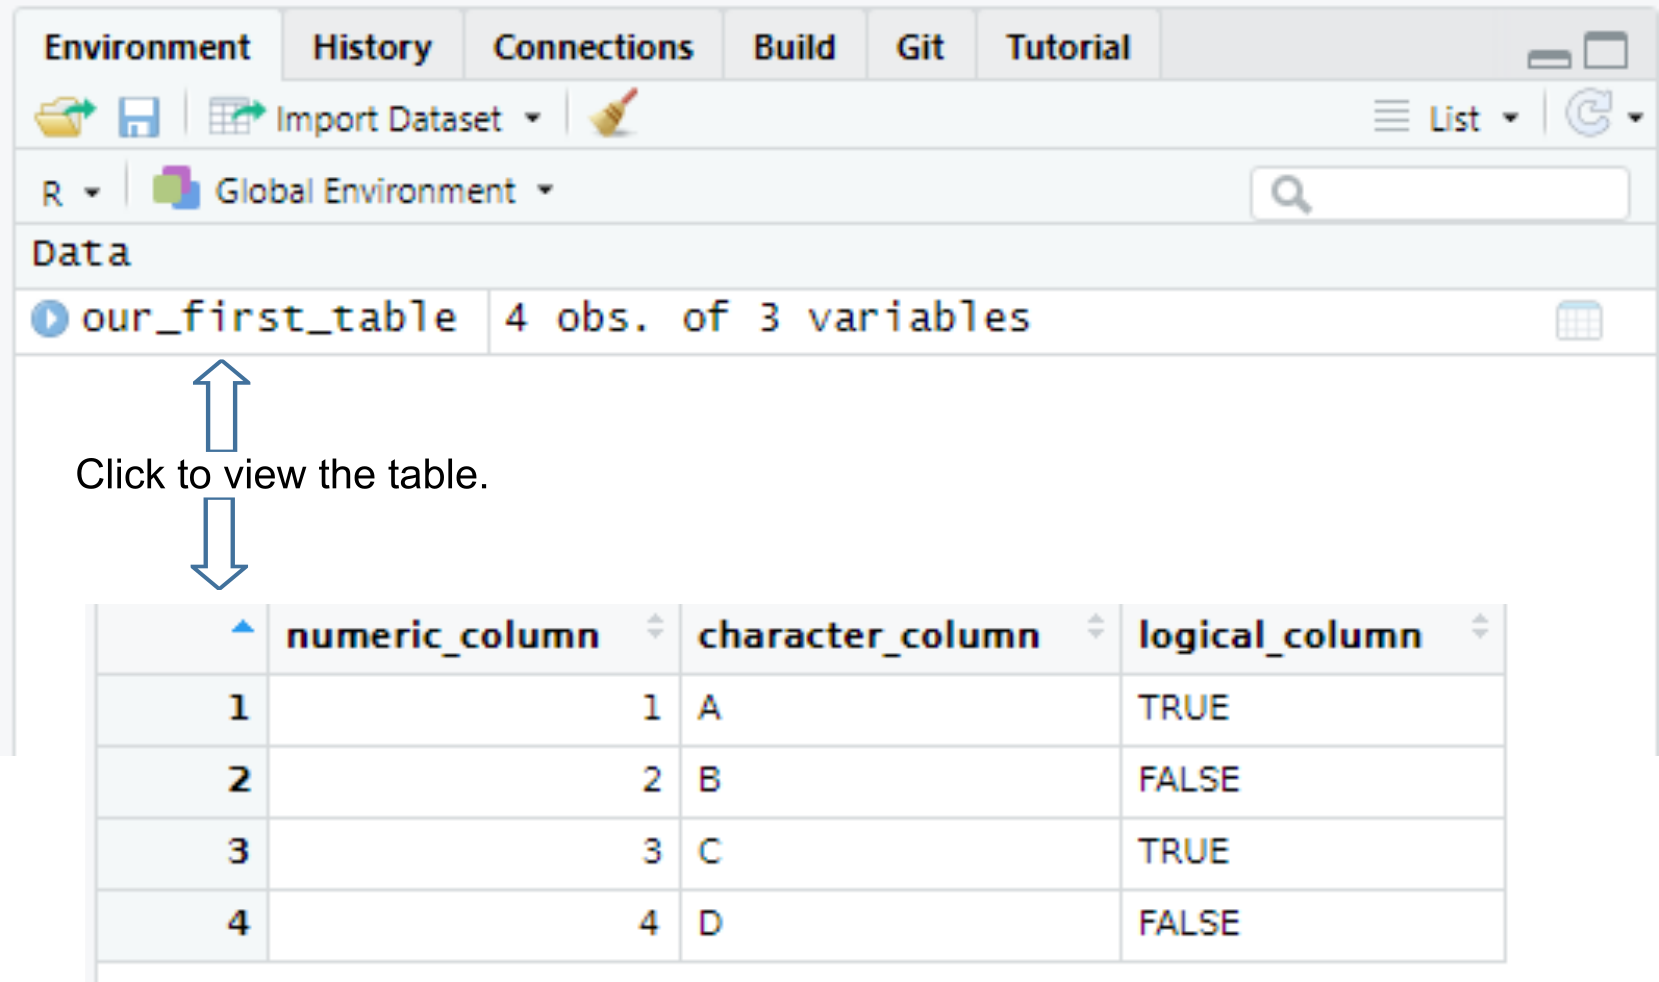
\includegraphics[width=1\linewidth]{images/viewing-table} \end{center}

Do exercise 3.

Because all columns in a table \textbf{must} have the same number of rows. This is similar to the process of \protect\hyperlink{different-length-vectors}{matching vectors' length} that you have learned the last time. However, it works automatically only if length of \emph{all} vectors is a multiple of the longest length. Thus, the example below will work, as the longest vector (\texttt{numeric\_column}) is 6, \texttt{character\_column} length is 3, so it will be repeated twice, and \texttt{logical\_column} length is 2 so it will be repeated thrice.

\begin{Shaded}
\begin{Highlighting}[]
\NormalTok{the\_table }\OtherTok{\textless{}{-}} \FunctionTok{data.frame}\NormalTok{(}\AttributeTok{numeric\_column =} \DecValTok{1}\SpecialCharTok{:}\DecValTok{6}\NormalTok{,                  }\CommentTok{\# length 6 }
                        \AttributeTok{character\_column =} \FunctionTok{c}\NormalTok{(}\StringTok{"A"}\NormalTok{, }\StringTok{"B"}\NormalTok{, }\StringTok{"C"}\NormalTok{),   }\CommentTok{\# length 3}
                        \AttributeTok{logical\_column =} \FunctionTok{c}\NormalTok{(}\ConstantTok{TRUE}\NormalTok{, }\ConstantTok{FALSE}\NormalTok{))       }\CommentTok{\# length 2}
\NormalTok{the\_table}
\end{Highlighting}
\end{Shaded}

\begin{verbatim}
##   numeric_column character_column logical_column
## 1              1                A           TRUE
## 2              2                B          FALSE
## 3              3                C           TRUE
## 4              4                A          FALSE
## 5              5                B           TRUE
## 6              6                C          FALSE
\end{verbatim}

If the simple \emph{multple-of-length} rule does not work, R (finally!) generates an error.

\begin{Shaded}
\begin{Highlighting}[]
\CommentTok{\# this will generate an error: arguments imply differing number of rows}
\NormalTok{the\_table }\OtherTok{\textless{}{-}} \FunctionTok{data.frame}\NormalTok{(}\AttributeTok{numeric\_column =} \DecValTok{1}\SpecialCharTok{:}\DecValTok{7}\NormalTok{,                 }\CommentTok{\# length 7}
                        \AttributeTok{character\_column =} \FunctionTok{c}\NormalTok{(}\StringTok{"A"}\NormalTok{, }\StringTok{"B"}\NormalTok{, }\StringTok{"C"}\NormalTok{))  }\CommentTok{\# length 3, cannot be multiplied by an integer to get 7}
\end{Highlighting}
\end{Shaded}

Do exercise 4.

Just as with the vectors, you can extract or modify only some elements (rows, columns, subsets) of a table. There are several ways to do it, as you can extract individual elements, individual columns, individual rows, or some rows and some columns. Subsetting tables is not the most exciting and fairly confusing topic but you need to understand it as in the R code that you will encounter different notations could be used interchangeably.

\hypertarget{extracting-a-single-vector-column-get-single-column}{%
\section{Extracting a single vector / column {[}\#get-single-column{]}}\label{extracting-a-single-vector-column-get-single-column}}

To access individual \emph{vectors} (a.k.a. columns or variables) use dollar notation \texttt{table\$column\_name} (this should be your default way) or \textbf{double} square brackets, \texttt{table{[}{[}column\_name{]}{]}} or \texttt{table{[}{[}column\_index{]}{]}}. Note that you cannot use multiple indexes (\texttt{c(1,\ 2)}) or slicing (e.g., \texttt{1:2}) with double square brackets. The important if subtle detail is that this notation returns a \emph{vector}, just a like one that you create via \texttt{c()} function.

\begin{Shaded}
\begin{Highlighting}[]
\NormalTok{our\_first\_table }\OtherTok{\textless{}{-}} \FunctionTok{data.frame}\NormalTok{(}\AttributeTok{numeric\_column =} \FunctionTok{c}\NormalTok{(}\DecValTok{1}\NormalTok{, }\DecValTok{2}\NormalTok{, }\DecValTok{3}\NormalTok{), }
                              \AttributeTok{character\_column =} \FunctionTok{c}\NormalTok{(}\StringTok{"A"}\NormalTok{, }\StringTok{"B"}\NormalTok{, }\StringTok{"C"}\NormalTok{),}
                              \AttributeTok{logical\_column =} \FunctionTok{c}\NormalTok{(}\ConstantTok{TRUE}\NormalTok{, F, T))}

\CommentTok{\# via $ notation}
\NormalTok{our\_first\_table}\SpecialCharTok{$}\NormalTok{numeric\_column}
\end{Highlighting}
\end{Shaded}

\begin{verbatim}
## [1] 1 2 3
\end{verbatim}

\begin{Shaded}
\begin{Highlighting}[]
\CommentTok{\# via name and double square brackets}
\NormalTok{our\_first\_table[[}\StringTok{\textquotesingle{}numeric\_column\textquotesingle{}}\NormalTok{]]}
\end{Highlighting}
\end{Shaded}

\begin{verbatim}
## [1] 1 2 3
\end{verbatim}

\begin{Shaded}
\begin{Highlighting}[]
\CommentTok{\# via index and double square brackets}
\NormalTok{our\_first\_table[[}\DecValTok{1}\NormalTok{]]}
\end{Highlighting}
\end{Shaded}

\begin{verbatim}
## [1] 1 2 3
\end{verbatim}

\begin{center}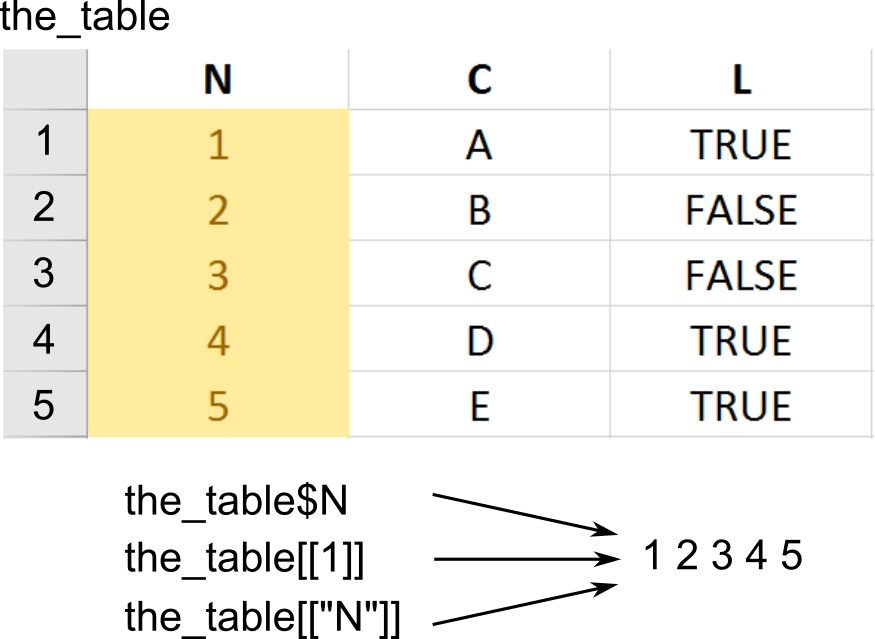
\includegraphics[width=1\linewidth]{images/table-column} \end{center}

\hypertarget{table-indexing}{%
\section{Extracting part of a table}\label{table-indexing}}

Alternatively, you can extract or access a rectangular part of the table via \textbf{single} square brackets. To get one or more columns you can use their names or indexes just as you did with vectors.

\begin{Shaded}
\begin{Highlighting}[]
\NormalTok{our\_first\_table }\OtherTok{\textless{}{-}} \FunctionTok{data.frame}\NormalTok{(}\AttributeTok{numeric\_column =} \FunctionTok{c}\NormalTok{(}\DecValTok{1}\NormalTok{, }\DecValTok{2}\NormalTok{, }\DecValTok{3}\NormalTok{), }
                              \AttributeTok{character\_column =} \FunctionTok{c}\NormalTok{(}\StringTok{"A"}\NormalTok{, }\StringTok{"B"}\NormalTok{, }\StringTok{"C"}\NormalTok{),}
                              \AttributeTok{logical\_column =} \FunctionTok{c}\NormalTok{(}\ConstantTok{TRUE}\NormalTok{, F, T))}

\CommentTok{\# via index}
\NormalTok{our\_first\_table[}\DecValTok{1}\NormalTok{]}
\end{Highlighting}
\end{Shaded}

\begin{verbatim}
##   numeric_column
## 1              1
## 2              2
## 3              3
\end{verbatim}

\begin{Shaded}
\begin{Highlighting}[]
\CommentTok{\# via name }
\NormalTok{our\_first\_table[}\StringTok{\textquotesingle{}numeric\_column\textquotesingle{}}\NormalTok{]}
\end{Highlighting}
\end{Shaded}

\begin{verbatim}
##   numeric_column
## 1              1
## 2              2
## 3              3
\end{verbatim}

\begin{Shaded}
\begin{Highlighting}[]
\CommentTok{\# via slicing}
\NormalTok{our\_first\_table[}\DecValTok{1}\SpecialCharTok{:}\DecValTok{2}\NormalTok{]}
\end{Highlighting}
\end{Shaded}

\begin{verbatim}
##   numeric_column character_column
## 1              1                A
## 2              2                B
## 3              3                C
\end{verbatim}

\begin{center}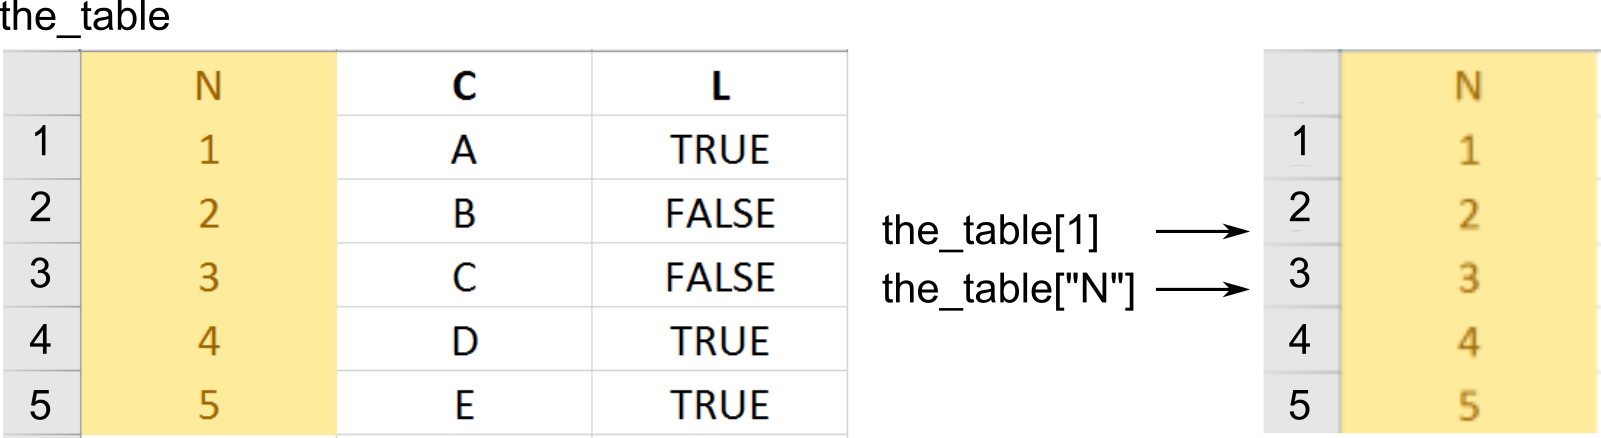
\includegraphics[width=1\linewidth]{images/table-subtable} \end{center}

Again, note that first two call get you a single-column table not a vector. You still need to use the column name to access its values.

\begin{Shaded}
\begin{Highlighting}[]
\NormalTok{our\_first\_table }\OtherTok{\textless{}{-}} \FunctionTok{data.frame}\NormalTok{(}\AttributeTok{numeric\_column =} \FunctionTok{c}\NormalTok{(}\DecValTok{1}\NormalTok{, }\DecValTok{2}\NormalTok{, }\DecValTok{3}\NormalTok{), }
                              \AttributeTok{character\_column =} \FunctionTok{c}\NormalTok{(}\StringTok{"A"}\NormalTok{, }\StringTok{"B"}\NormalTok{, }\StringTok{"C"}\NormalTok{),}
                              \AttributeTok{logical\_column =} \FunctionTok{c}\NormalTok{(}\ConstantTok{TRUE}\NormalTok{, F, T))}

\NormalTok{table\_copy }\OtherTok{\textless{}{-}}\NormalTok{ our\_first\_table[}\DecValTok{1}\NormalTok{]}
\NormalTok{table\_copy}\SpecialCharTok{$}\NormalTok{numeric\_column}
\end{Highlighting}
\end{Shaded}

\begin{verbatim}
## [1] 1 2 3
\end{verbatim}

To select a subset rows and columns you write \texttt{table{[}rows,\ column{]}}. If you omit either rows or columns this implies that you want \emph{all} rows or columns.

\begin{Shaded}
\begin{Highlighting}[]
\NormalTok{our\_first\_table }\OtherTok{\textless{}{-}} \FunctionTok{data.frame}\NormalTok{(}\AttributeTok{numeric\_column =} \FunctionTok{c}\NormalTok{(}\DecValTok{1}\NormalTok{, }\DecValTok{2}\NormalTok{, }\DecValTok{3}\NormalTok{), }
                              \AttributeTok{character\_column =} \FunctionTok{c}\NormalTok{(}\StringTok{"A"}\NormalTok{, }\StringTok{"B"}\NormalTok{, }\StringTok{"C"}\NormalTok{),}
                              \AttributeTok{logical\_column =} \FunctionTok{c}\NormalTok{(}\ConstantTok{TRUE}\NormalTok{, F, T))}

\CommentTok{\# getting ALL rows for the FIRST column {-}\textgreater{} this gives you a VECTOR}
\NormalTok{our\_first\_table[, }\DecValTok{1}\NormalTok{]}
\end{Highlighting}
\end{Shaded}

\begin{verbatim}
## [1] 1 2 3
\end{verbatim}

\begin{Shaded}
\begin{Highlighting}[]
\CommentTok{\# getting FIRST row for ALL columns {-}\textgreater{} this gives you DATA.FRAME}
\NormalTok{our\_first\_table[}\DecValTok{1}\NormalTok{, ]}
\end{Highlighting}
\end{Shaded}

\begin{verbatim}
##   numeric_column character_column logical_column
## 1              1                A           TRUE
\end{verbatim}

\begin{Shaded}
\begin{Highlighting}[]
\CommentTok{\# ALL rows and ALL columns, equivalent to just writing \textasciigrave{}our\_first\_table\textasciigrave{} or \textasciigrave{}our\_first\_table[]\textasciigrave{}}
\NormalTok{our\_first\_table[,]}
\end{Highlighting}
\end{Shaded}

\begin{verbatim}
##   numeric_column character_column logical_column
## 1              1                A           TRUE
## 2              2                B          FALSE
## 3              3                C           TRUE
\end{verbatim}

\begin{Shaded}
\begin{Highlighting}[]
\CommentTok{\# getting SECOND element of the THIRD column}
\NormalTok{our\_first\_table[}\DecValTok{2}\NormalTok{, }\DecValTok{3}\NormalTok{]}
\end{Highlighting}
\end{Shaded}

\begin{verbatim}
## [1] FALSE
\end{verbatim}

\begin{Shaded}
\begin{Highlighting}[]
\CommentTok{\# getting first two elements of the logical\_column}
\NormalTok{our\_first\_table[}\DecValTok{1}\SpecialCharTok{:}\DecValTok{2}\NormalTok{, }\StringTok{"logical\_column"}\NormalTok{]}
\end{Highlighting}
\end{Shaded}

\begin{verbatim}
## [1]  TRUE FALSE
\end{verbatim}

\begin{center}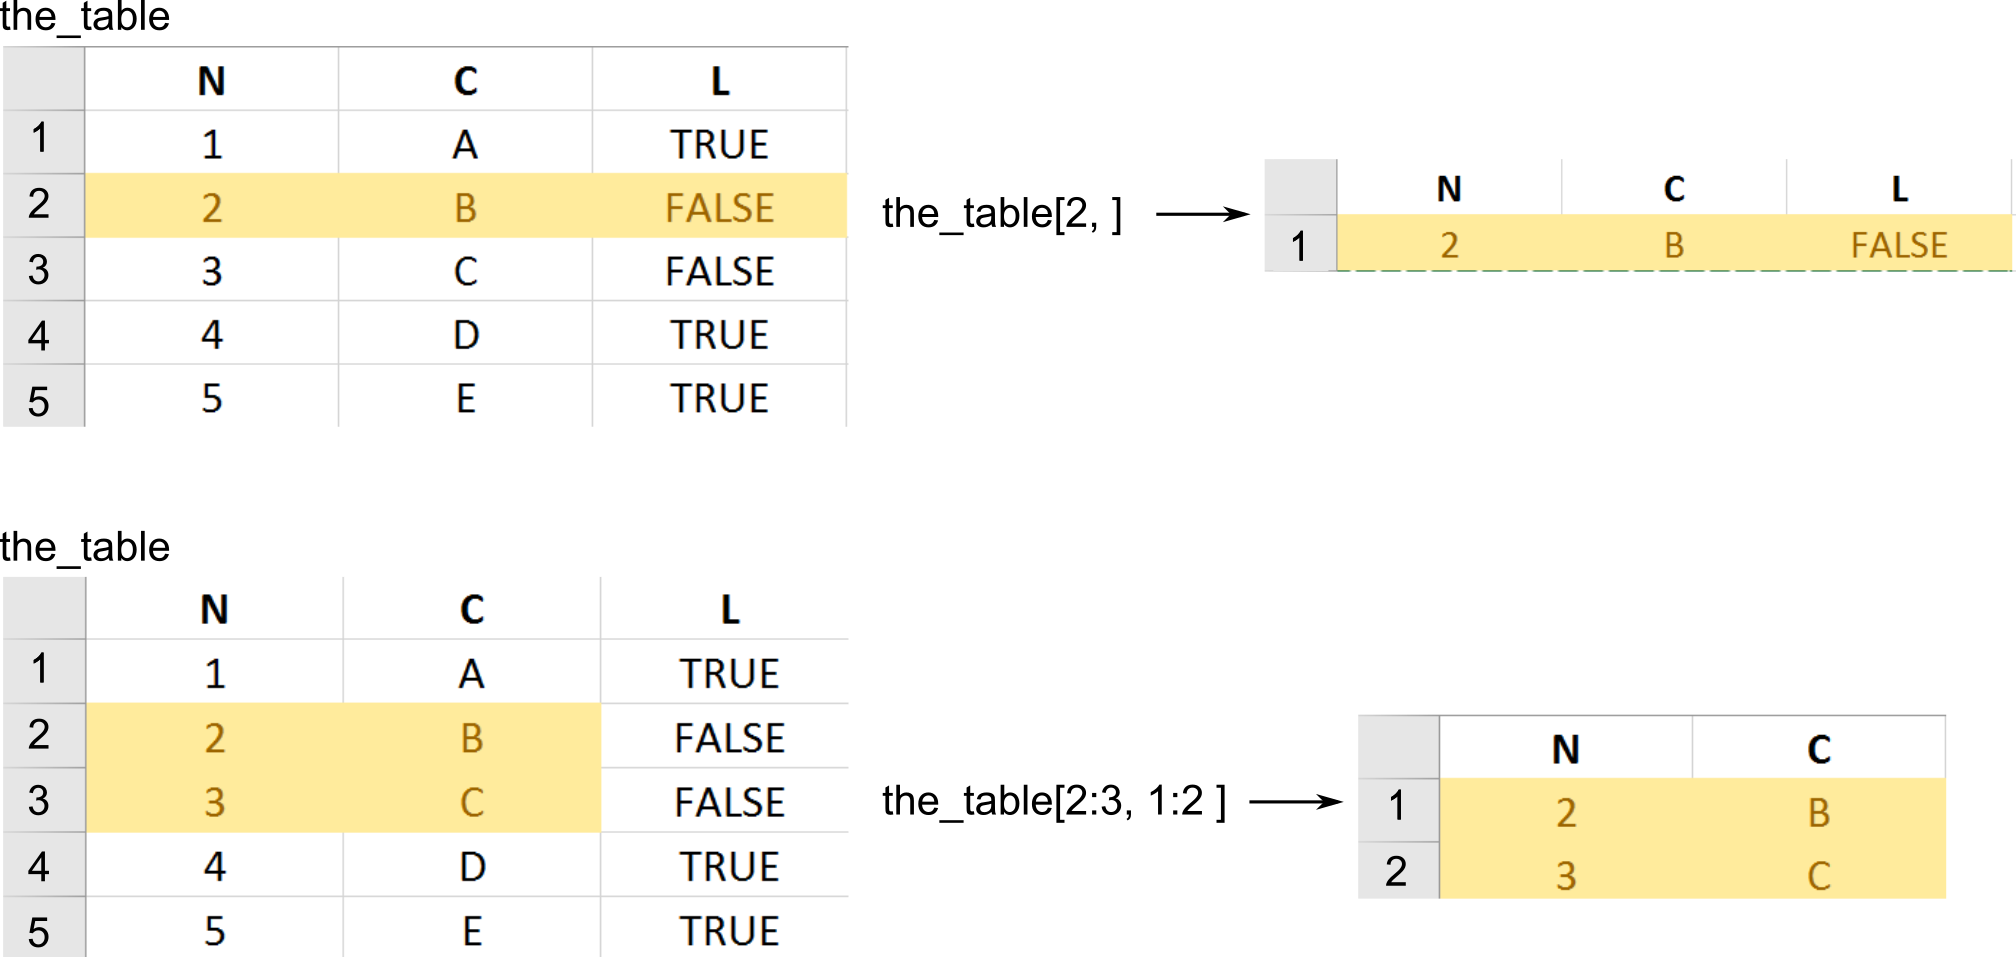
\includegraphics[width=1\linewidth]{images/table-rows-columns} \end{center}

Do exercise 5.

\hypertarget{library}{%
\section{Using libraries}\label{library}}

There is a better way to construct a table but to use it, we need to first import a library that implements it. As with most modern programming languages, the real power of R is not what comes bundled with it (very little, as a matter of fact) but community developed libraries that extend it. We already discussed how you \protect\hyperlink{install.packages}{install libraries}. For that you use \href{https://www.rdocumentation.org/packages/base/versions/3.6.2/topics/library}{library()} function (it has a sister function \texttt{require()} but it should be used inside functions and packages not in scripts or notebooks). So, to use \emph{tidyverse} library that you already installed, you simply write

\begin{Shaded}
\begin{Highlighting}[]
\FunctionTok{library}\NormalTok{(tidyverse)}
\CommentTok{\# or}
\FunctionTok{library}\NormalTok{(}\StringTok{"tidyverse"}\NormalTok{)}
\end{Highlighting}
\end{Shaded}

One thing to keep in mind is that if you import two libraries that have a function with same name, the function from the \emph{latter} package will overwrite (mask) the function from the former. You will get a warning but if you miss it, it may be very confusing. My favorite stumbling block are functions \texttt{filter()} from \texttt{dplyr} package (we will use it extensively, as it filters a table by row) and \texttt{filter()} function from \texttt{signal} package (applies a filter to a time-series). This overwriting of one function by another can lead to very odd looking mistakes. In my case I though I was using \texttt{dplyr::filter()} and could not understand the error message I was getting, it it took me an hour to figure it out the first time. Here are the warnings I should have paid attention to.

\begin{Shaded}
\begin{Highlighting}[]
\FunctionTok{library}\NormalTok{(dplyr)}
\end{Highlighting}
\end{Shaded}

\begin{verbatim}
## 
## Attaching package: 'dplyr'
\end{verbatim}

\begin{verbatim}
## The following objects are masked from 'package:stats':
## 
##     filter, lag
\end{verbatim}

\begin{verbatim}
## The following objects are masked from 'package:base':
## 
##     intersect, setdiff, setequal, union
\end{verbatim}

Thus, keep that in mind or, better still, explicitly mention which package the function is coming from via \texttt{library::function()} notation. In this case, you will use the function that you are interested in and need not to worry about other functions with the same name that may conflict with it. In general, it is a good idea to \emph{always} disambiguate function via library but in practice it may make your code hard to read by littering it with \texttt{library::} prefixes. Thus, you will need to find a balance between disambiguation and readability.

\begin{Shaded}
\begin{Highlighting}[]
\FunctionTok{library}\NormalTok{(tibble)}

\CommentTok{\# imported from the library into the global environment}
\FunctionTok{print}\NormalTok{(}\FunctionTok{tribble}\NormalTok{(}\SpecialCharTok{\textasciitilde{}}\NormalTok{a, }\DecValTok{1}\NormalTok{))}
\end{Highlighting}
\end{Shaded}

\begin{verbatim}
## # A tibble: 1 x 1
##       a
##   <dbl>
## 1     1
\end{verbatim}

\begin{Shaded}
\begin{Highlighting}[]
\CommentTok{\# used directly from the package}
\NormalTok{tibble}\SpecialCharTok{::}\FunctionTok{tribble}\NormalTok{(}\SpecialCharTok{\textasciitilde{}}\NormalTok{a, }\DecValTok{1}\NormalTok{)}
\end{Highlighting}
\end{Shaded}

\begin{verbatim}
## # A tibble: 1 x 1
##       a
##   <dbl>
## 1     1
\end{verbatim}

When using a notebook (so, in our case, always) put the libraries into \emph{setup} chunk of the notebook. This ensures that your libraries are always initialized, even if you first run some other chunk. Word of advice, keep you library list in alphabetical order. Because libraries are very specialized, you will need quite a few of them for a typical analysis. Keeping them alphabetically organized makes it easier to see whether you imported the required library and whether you need to install a new one.

\hypertarget{tibble}{%
\section{Tibble, a better data.frame}\label{tibble}}

Although the \texttt{data.frame()} function is the default way of creating a table, it is a legacy implementation with numerous shortcomings. Tidyverse implemented its own version of the table called \href{https://tibble.tidyverse.org/}{tibble()} that provides a more rigorous control and more consistent behavior. For example, it allows you to use any symbols for the columns names (including spaces), prints out only beginning of the table rather than entire table, etc. It also gives more warnings. If you try to access a non-existing column both \texttt{data.frame()} and \texttt{tibble()} will return \texttt{NULL} but the former will do it silently, whereas the latter will complain.

\begin{Shaded}
\begin{Highlighting}[]
\FunctionTok{library}\NormalTok{(tibble)}

\CommentTok{\# data.frame will return NULL silently}
\NormalTok{df }\OtherTok{\textless{}{-}} \FunctionTok{data.frame}\NormalTok{(}\AttributeTok{b =} \DecValTok{1}\NormalTok{)}
\FunctionTok{print}\NormalTok{(df}\SpecialCharTok{$}\NormalTok{A)}
\end{Highlighting}
\end{Shaded}

\begin{verbatim}
## NULL
\end{verbatim}

\begin{Shaded}
\begin{Highlighting}[]
\CommentTok{\# data.frame will return NULL for a variable that does not exist}

\NormalTok{tbl }\OtherTok{\textless{}{-}} \FunctionTok{tibble}\NormalTok{(}\AttributeTok{b =} \DecValTok{1}\NormalTok{)}
\FunctionTok{print}\NormalTok{(tbl}\SpecialCharTok{$}\NormalTok{A)}
\end{Highlighting}
\end{Shaded}

\begin{verbatim}
## Warning: Unknown or uninitialised column: `A`.
\end{verbatim}

\begin{verbatim}
## NULL
\end{verbatim}

In short, \texttt{tibble()} provides a more robust version of a \texttt{data.frame} but otherwise behaves (mostly) identically to it. Thus, it should be your default choice for a table.

\hypertarget{tribble}{%
\section{Tribble, table from text}\label{tribble}}

The tibble package also provides an easier to read way of constructing tables via the \href{https://tibble.tidyverse.org/reference/tribble.html}{tribble()} function. Here, you use tilde to specify column names, and then write the content row-by-row.

\begin{Shaded}
\begin{Highlighting}[]
\FunctionTok{tribble}\NormalTok{(}
    \SpecialCharTok{\textasciitilde{}}\NormalTok{x, }\SpecialCharTok{\textasciitilde{}}\NormalTok{y,}
    \DecValTok{1}\NormalTok{,  }\StringTok{"a"}\NormalTok{,}
    \DecValTok{2}\NormalTok{,  }\StringTok{"b"}
\NormalTok{)}
\end{Highlighting}
\end{Shaded}

\begin{verbatim}
## # A tibble: 2 x 2
##       x y    
##   <dbl> <chr>
## 1     1 a    
## 2     2 b
\end{verbatim}

Do exercise 6.

\hypertarget{data}{%
\section{Reading example tables}\label{data}}

One of the great things about R is that most packages come with an example data set that illustrates their function. You can see the list of some of them \href{https://www.rdocumentation.org/packages/datasets}{here}. In case of example data set, you need to import the library it is part of and then load them by writing \texttt{data(tablename)}. For example, to use use \texttt{mpg} data on fuel economy from \texttt{ggplot2} package, you need to import the library first, and then call \texttt{data(mpg)}.

\begin{Shaded}
\begin{Highlighting}[]
\FunctionTok{library}\NormalTok{(ggplot2)}
\FunctionTok{data}\NormalTok{(mpg) }\CommentTok{\# this create a "promise" of the data}
\FunctionTok{print}\NormalTok{(mpg) }\CommentTok{\# any action on the promise leads to data appearing in the environment}
\end{Highlighting}
\end{Shaded}

\begin{verbatim}
## # A tibble: 234 x 11
##    manufacturer model    displ  year   cyl trans   drv     cty   hwy fl    class
##    <chr>        <chr>    <dbl> <int> <int> <chr>   <chr> <int> <int> <chr> <chr>
##  1 audi         a4         1.8  1999     4 auto(l~ f        18    29 p     comp~
##  2 audi         a4         1.8  1999     4 manual~ f        21    29 p     comp~
##  3 audi         a4         2    2008     4 manual~ f        20    31 p     comp~
##  4 audi         a4         2    2008     4 auto(a~ f        21    30 p     comp~
##  5 audi         a4         2.8  1999     6 auto(l~ f        16    26 p     comp~
##  6 audi         a4         2.8  1999     6 manual~ f        18    26 p     comp~
##  7 audi         a4         3.1  2008     6 auto(a~ f        18    27 p     comp~
##  8 audi         a4 quat~   1.8  1999     4 manual~ 4        18    26 p     comp~
##  9 audi         a4 quat~   1.8  1999     4 auto(l~ 4        16    25 p     comp~
## 10 audi         a4 quat~   2    2008     4 manual~ 4        20    28 p     comp~
## # ... with 224 more rows
\end{verbatim}

\hypertarget{readr}{%
\section{Reading csv files}\label{readr}}

So far we covered creating a table by hand via \texttt{data.frame()}, \texttt{tibble()}, or \texttt{tribble()} functions and loading an example table from a package via \texttt{data()} function. More commonly, you will need to read a table from an external file. These files can come in many formats because they are generated by different experimental software. Below, you will see how to handle those but my recommendation is to always store your data in a csv (\href{https://en.wikipedia.org/wiki/Comma-separated_values}{Comma-separated values}) files. These are simple plain text files, which means you can open them in any text editor, with each line representing a single row (typically, top row contains column names) with individual columns separated by some symbol or symbols. Typical separators are a comma (hence, the name), a semicolon (this is frequently used in Germany, with comma serving as a decimal point), a tabulator, or even a space symbol. Here is an example of such file

\begin{verbatim}
Participant,Block,Trial,Contrast,Correct
A1,1,1,0.5,TRUE
A1,1,2,1.0,TRUE
A1,1,2,0.05,FALSE
...
\end{verbatim}

that is turned into a table when loaded

\begin{center}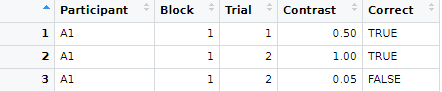
\includegraphics[width=0.7\linewidth]{images/results-csv-table} \end{center}

There are several ways of reading CSV files in R. The default way by using \href{https://stat.ethz.ch/R-manual/R-devel/library/utils/html/read.table.html}{read.csv()} function that comes has different versions optimized for different combinations of the decimal point and separator symbols, e.g.~\texttt{read.csv2()} assumes a comma for the decimal point and semicolon as a separator. However, a better way is to use \href{https://readr.tidyverse.org/}{readr} library that implements same functions. Names of the functions are slightly different with underscore replacing the dot, so \texttt{readr::read\_csv()} is a replacement for \texttt{read.csv()}. These are faster (although it will be noticeable only on large data sets), do not convert text to factor variables (we will talk about factors later but this default conversion by \texttt{read.csv()} can be very confusing), etc.

However, most important difference between \texttt{read.csv()} and \texttt{read\_csv()} is they constraint the content of a CSV file. \texttt{read.csv()} has not assumptions about which columns are in the file and what their value types are. It simply reads them as is, \emph{silently} guessing their type.

\begin{Shaded}
\begin{Highlighting}[]
\NormalTok{results }\OtherTok{\textless{}{-}} \FunctionTok{read.csv}\NormalTok{(}\StringTok{"data/example.csv"}\NormalTok{)}
\NormalTok{results}
\end{Highlighting}
\end{Shaded}

\begin{verbatim}
##   Participant Block Trial Contrast Correct
## 1          A1     1     1     0.50    TRUE
## 2          A1     1     2     1.00    TRUE
## 3          A1     1     2     0.05   FALSE
\end{verbatim}

You can use \texttt{read\_csv()} the same way and it will work the same way but warn you about the table structure it deduced.

\begin{Shaded}
\begin{Highlighting}[]
\NormalTok{results }\OtherTok{\textless{}{-}}\NormalTok{ readr}\SpecialCharTok{::}\FunctionTok{read\_csv}\NormalTok{(}\StringTok{"data/example.csv"}\NormalTok{)}
\end{Highlighting}
\end{Shaded}

\begin{verbatim}
## 
## -- Column specification --------------------------------------------------------
## cols(
##   Participant = col_character(),
##   Block = col_double(),
##   Trial = col_double(),
##   Contrast = col_double(),
##   Correct = col_logical()
## )
\end{verbatim}

\begin{Shaded}
\begin{Highlighting}[]
\NormalTok{results}
\end{Highlighting}
\end{Shaded}

\begin{verbatim}
## # A tibble: 3 x 5
##   Participant Block Trial Contrast Correct
##   <chr>       <dbl> <dbl>    <dbl> <lgl>  
## 1 A1              1     1     0.5  TRUE   
## 2 A1              1     2     1    TRUE   
## 3 A1              1     2     0.05 FALSE
\end{verbatim}

This annoying \emph{Column specification} print out, which gets even more annoying if you need to read many CSV files, is there for a reason: it wants to annoy you! Because the only way to turn it off and stop being annoyed is to specify the column structure yourself via \texttt{col\_types} parameter. As a matter of fact, the print out you get is where, so you can take a look at it, adjust it, if necessary, and copy-paste to the \texttt{read\_csv} call. By default, it suggested \texttt{double} values for \texttt{Block} and \texttt{Trial} but we know they are integers, so we can copy-paste the suggested structure, replace \texttt{col\_double()} with \texttt{col\_integer()} and read the table without a warning.

\begin{Shaded}
\begin{Highlighting}[]
\FunctionTok{library}\NormalTok{(readr)}
\NormalTok{results }\OtherTok{\textless{}{-}} \FunctionTok{read\_csv}\NormalTok{(}\StringTok{"data/example.csv"}\NormalTok{, }
                    \AttributeTok{col\_types =} \FunctionTok{cols}\NormalTok{(}\AttributeTok{Participant =} \FunctionTok{col\_character}\NormalTok{(),}
                                     \AttributeTok{Block =} \FunctionTok{col\_integer}\NormalTok{(), }\CommentTok{\# read\_csv suggested col\_double() but we know better}
                                     \AttributeTok{Trial =} \FunctionTok{col\_integer}\NormalTok{(), }\CommentTok{\# read\_csv suggested col\_double() but we know better}
                                     \AttributeTok{Contrast =} \FunctionTok{col\_double}\NormalTok{(),}
                                     \AttributeTok{Correct =} \FunctionTok{col\_logical}\NormalTok{()))}
\NormalTok{results}
\end{Highlighting}
\end{Shaded}

\begin{verbatim}
## # A tibble: 3 x 5
##   Participant Block Trial Contrast Correct
##   <chr>       <int> <int>    <dbl> <lgl>  
## 1 A1              1     1     0.5  TRUE   
## 2 A1              1     2     1    TRUE   
## 3 A1              1     2     0.05 FALSE
\end{verbatim}

You may feel that this a lot of extra work just to suppress an annoying but, ultimately, harmless warning. Your code will work with or without it, right? Well, \emph{hopefully} it will but you probably want to \emph{know} that it will work not \emph{hope} for it. Imagine that you accidentally overwrote your experimental data file with data from a different experiment (that happens more often than one would want). You still have \texttt{results.csv} file in your project folder and so the \texttt{read.csv()} will read it as is (it does not know what should be in that file) and your analysis code will fail in some mysterious ways at a much later point (because, remember, if you try to access a column/variable that does not exist in the table, you just get \texttt{NULL} rather than an error). You will eventually trace it back to the wrong data file but that will cost time and nerves. However, if you specify the column structure in \texttt{read\_csv()} it will show warning, if the file does not match the description. It would warn about wrong column names (\texttt{TheBlock} in the example below) and about wrong type (it does not like \texttt{TRUE}/\texttt{FALSE} in a column it expected to find integers in).

\begin{Shaded}
\begin{Highlighting}[]
\FunctionTok{library}\NormalTok{(readr)}
\NormalTok{results }\OtherTok{\textless{}{-}} \FunctionTok{read\_csv}\NormalTok{(}\StringTok{"data/example.csv"}\NormalTok{, }
                    \AttributeTok{col\_types =} \FunctionTok{cols}\NormalTok{(}\AttributeTok{Participant =} \FunctionTok{col\_character}\NormalTok{(),}
                                     \AttributeTok{TheBlock =} \FunctionTok{col\_integer}\NormalTok{(), }\CommentTok{\# read\_csv suggested col\_double() but we know better}
                                     \AttributeTok{Trial =} \FunctionTok{col\_integer}\NormalTok{(), }\CommentTok{\# read\_csv suggested col\_double() but we know better}
                                     \AttributeTok{Contrast =} \FunctionTok{col\_double}\NormalTok{(),}
                                     \AttributeTok{Correct =} \FunctionTok{col\_integer}\NormalTok{()))}
\end{Highlighting}
\end{Shaded}

\begin{verbatim}
## Warning: The following named parsers don't match the column names: TheBlock
\end{verbatim}

\begin{verbatim}
## Warning: 3 parsing failures.
## row     col   expected actual               file
##   1 Correct an integer  TRUE  'data/example.csv'
##   2 Correct an integer  TRUE  'data/example.csv'
##   3 Correct an integer  FALSE 'data/example.csv'
\end{verbatim}

Personally, I would prefer for \texttt{read\_csv()} to fail in cases like these but having a nice red warning is already very helpful to quickly detect the problem with your data (and if your data is wrong, your whole analysis is meaningless). Thus, \emph{always} use \texttt{read\_} rather than \texttt{read.} functions and \emph{always} specify the table structure. The lazy, and my preferred, way to do it, is to first read the file without specifying the structure and copy-paste-edit the warning column-specification message into the code.

Do exercise 7, you need \href{data/face_rank.csv}{face\_rank.csv} file for it. Download it and place it in the project folder. \emph{Warning}, if you use Chrome or any Chromium-based browsers like MS Edge, Opera, etc. they might, for some odd reason, automatically \emph{rename it} into \emph{face\_rank.xls} during the download. Just rename it back to \emph{face\_rank.csv}, because the file is not converted to an Excel, it is only the extension that gets changed (why? No idea, ask Google!).

\hypertarget{readxl}{%
\section{Reading Excel files}\label{readxl}}

There are several libraries that allow you to read Excel files directly. My personal preference is \href{https://readxl.tidyverse.org/}{readxl} package, which is part of the Tidyverse. Warning, it will be installed as part of the Tidyverse (i.e., when you typed \texttt{install.packages(tidyverse)}) but you still need to import it explicitly via \texttt{library(readxl)}. Because an Excel file has many sheets, by default the \texttt{read\_excel()} function reads the \emph{first} sheet but you can specify it via a \texttt{sheet} parameter using its index \texttt{read\_excel("my\_excel\_file.xls",\ sheet=2)} or name \texttt{read\_excel("my\_excel\_file.xls",\ sheet="addendum")}.

Do exercise 8, you need \href{data/face_rank.xlsx}{face\_rank.xlsx} file for it.

You can read about further options at the package's website but I would generally discourage you from using Excel for your work and, definitely, for your data analysis. Because, you see, Excel is very smart and it can figure out the \emph{true} meaning and type of columns by itself. The fact that you might disagree is your problem. Excel knows what is best for you. The easiest way to screw a CSV file up is to open it in Excel and immediately save it. The file name will remain the same but Excel will ``adjust'' the content as it feels is better for you (you don't need to be consulted with). If you think I am exaggerating, read this \href{https://www.theverge.com/2020/8/6/21355674/human-genes-rename-microsoft-excel-misreading-dates}{article} at The Verge on how Excel messed up thousands of human genome data tables by turning some values into dates (because why not?). So now the entire community is \emph{renaming} some genes because it is easier to waste literally thousands of man-hours on that than to fix Excel. In short, friends don't let friends use Excel.

\hypertarget{reading-files-from-other-programs}{%
\section{Reading files from other programs}\label{reading-files-from-other-programs}}

World is a very diverse place, so you are likely to encounter a wide range of data files generated by Matlab, SPSS, SAS, etc. There are two ways to import the data. First, that I would recommend, use the original program (Matlab, SPSS, SAS, etc.) to export data as a CSV file. Every program can read and write CSV, so it a good common ground. Moreover, this is simple format with no embedded formulas (as in Excel), service structures, etc. Finally, if you store your data in CSV, you do not need a special program to work with it. In short, unless you have a good reason, store your data in CSV files.

However, sometimes you have a file but you do not have the program (Matlab, SPSS, SAS, etc.). This is the second way, when you can use various R libaries, starting with \href{https://www.rdocumentation.org/packages/foreign}{foreign}, which can handle most typical cases, e.g., SPSS, SAS, State, or Minitab. The problem here, is that all the programs differ in the internal file formats and what exactly is included. For example, when importing from an SPSS sav-file via \href{https://www.rdocumentation.org/packages/foreign/versions/0.8-80/topics/read.spss}{read.spss} you will get a list with various components rather than a data.frame. You can force the function to convert everything to a single table via \texttt{to.data.frame=TRUE} option but you may lose some information. Bottom line, you need to be extra careful when importing from other formats and the safest way is to ensure complete and full export of the data to a CSV from the original program.

\hypertarget{wrap-up-1}{%
\section{Wrap up}\label{wrap-up-1}}

We have started with vectors and now extended them to tables. Next time, we will look at how to visualize the data using The Grammar of Graphics approach.

\hypertarget{ggplot2}{%
\chapter{Grammar of Graphics}\label{ggplot2}}

In previous seminar, you have learned about tables that are the main way of representing data in psychological research and in R. In the following seminars, you will learn how to manipulate the data in these tables: change it, aggregate or transform individual groups of data, use it for statistical analysis. But before that you need to understand how to store your data in the table in the optimal way. First, I will introduce the idea of \emph{tidy data}, the concept that gave \href{https://www.tidyverse.org/}{Tidyverse} its name. Next, we will see how tidy data helps you visualize the relationships between variables. Don't forget to download the \href{notebooks/Seminar\%2004\%20-\%20ggplot2.Rmd}{notebook}.

\hypertarget{tidydata}{%
\section{Tidy data}\label{tidydata}}

The tidy data follows \href{https://r4ds.had.co.nz/tidy-data.html}{three rules}:

\begin{itemize}
\tightlist
\item
  variables are in columns,
\item
  observations are in rows,
\item
  values are in cells.
\end{itemize}

This probably sound very straightforward to the point that you wonder ``Can a table not by tidy?'' As a matter of fact \emph{a lot} of typical results of psychological experiments are not tidy. Imagine an experiment where participants rated a face on symmetry, attractiveness, and trustworthiness. Typically (at least in my experience), the data will stored as follows:

\begin{tabular}{c|c|c|c|c}
\hline
Participant & Face & Symmetry & Attractiveness & Trustworthiness\\
\hline
1 & M1 & 6 & 4 & 3\\
\hline
1 & M2 & 4 & 7 & 6\\
\hline
2 & M1 & 5 & 2 & 1\\
\hline
2 & M2 & 3 & 7 & 2\\
\hline
\end{tabular}

This is a very typical table optimized for \emph{humans}. A single row contains all responses about a single face, so it is easy to visually compare responses of individual observers. Often, the table is even wider so that a single row holds all responses from a single observer (in my experience, a lot of online surveys produce data in this format).

\begin{tabular}{c|c|c|c|c|c|c}
\hline
Participant & M1.Symmetry & M1.Attractiveness & M1.Trustworthiness & M2.Symmetry & M2.Attractiveness & M2.Trustworthiness\\
\hline
1 & 6 & 4 & 3 & 4 & 7 & 6\\
\hline
2 & 5 & 2 & 1 & 3 & 7 & 2\\
\hline
\end{tabular}

So, what is wrong with it? Don't we have variables in columns, observations in rows, and values in cells? Not really. You can already see it when comparing the two tables above. The \emph{face} identity is a variable, however, in the second table it is hidden in column names. Some columns are about face \texttt{M1}, other columns are about \texttt{M2}, etc. So, if you are interested in analyzing symmetry judgments across all faces and participants, you will need to select all columns that end with \texttt{.Symmetry} and figure out a way to extract the face identity from columns' names. Thus, face \emph{is} a variable but is not a column in the second table.

Then, what about the first table, which has \texttt{Face} as a column, is it tidy? The short answer: Not really but that depends on your goals as well! In the experiment, we collected \emph{responses} (these are numbers in cells) for different type of \emph{judgments}. The latter are a variable but it is hidden in column names. Thus, a \emph{tidy} table for this data would be

\begin{tabular}{c|c|c|c|c}
\hline
Participant & Face & Trustworthiness & Judgment & Response\\
\hline
1 & M1 & 3 & Symmetry & 6\\
\hline
1 & M1 & 3 & Attractiveness & 4\\
\hline
1 & M2 & 6 & Symmetry & 4\\
\hline
1 & M2 & 6 & Attractiveness & 7\\
\hline
2 & M1 & 1 & Symmetry & 5\\
\hline
2 & M1 & 1 & Attractiveness & 2\\
\hline
2 & M2 & 2 & Symmetry & 3\\
\hline
2 & M2 & 2 & Attractiveness & 7\\
\hline
\end{tabular}

This table is (very) tidy and it makes it easy to group data by every different combination of variables (e.g.~per face and judgment, per participant and judgment), perform statistical analysis, etc. However, it may not always be the best way to represent the data. For example, if you would like to model \texttt{Trustworthiness} using \texttt{Symmetry} and \texttt{Attractiveness} as predictors, when the first table is more suitable. At the end, the table structure must fit your needs, not the other way around. Still, what you probably want is a \emph{tidy} table because it is best suited for most things you will want to do with the data and because it makes it easy to transform the data to match your specific needs (e.g., going from the third table to the first one via pivoting).

Most data you will get from experiments will not be tidy. We will spent quite some time in learning how to tidy it up but first let us see how an already tidy data makes it easy to visualize relationships in it.

\hypertarget{ggplot2-1}{%
\section{ggplot2}\label{ggplot2-1}}

\href{https://ggplot2.tidyverse.org/}{ggplot2} package is my main tool for data visualization in R. ggplot2 tends to make really good looking production-ready plots (this is not a given, a default-looking Matlab plot is, or used to be when I used Matlab, pretty ugly). Hadley Wickham was influenced by works of \href{https://www.edwardtufte.com/tufte/}{Edward Tufte} when developing ggplot2. Although the aesthetic aspect goes beyond our seminar (although, if you are interested, I might make a Christmas-special on that), if you will need to visualize data in the future, I strongly recommend reading Tufte's books. In fact, it is such an informative and aesthetically pleasing experience that I would recommend reading them in any case.

More importantly, ggplot2 uses a grammar-based approach of describing a plot that makes it conceptually different from most other software such as Matlab, Matplotlib in Python, etc. A plot in \emph{ggplot2} is described in three parts:

\begin{enumerate}
\def\labelenumi{\arabic{enumi}.}
\tightlist
\item
  Aesthetics: Relationship between data and visual properties that define working space of the plot (which variables map on axes, color, size, fill, etc.).
\item
  Geometrical primitives that visualize your data (points, lines, error bars, etc.) that are \emph{added} to the plot.
\item
  Other properties of the plot (scaling of axes, labels, annotations, etc.) that are \emph{added} to the plot.
\end{enumerate}

You always need the first one. But you do not need to specify the other two, even though a plot without geometry in it looks very empty. Let us start with a very simple artificial example table below.

\begin{tabular}{l|r|r}
\hline
Condition & Intensity & Response\\
\hline
A & 1 & 0.0496272\\
\hline
B & 1 & -1.5360443\\
\hline
C & 1 & -4.5436258\\
\hline
A & 2 & 1.3026641\\
\hline
B & 2 & -1.7912486\\
\hline
C & 2 & -2.7475456\\
\hline
A & 3 & 1.5018363\\
\hline
B & 3 & -1.1777133\\
\hline
C & 3 & -3.0938807\\
\hline
A & 4 & 3.0447694\\
\hline
B & 4 & 1.3077832\\
\hline
C & 4 & -1.4666246\\
\hline
A & 5 & 4.2699611\\
\hline
B & 5 & 1.8204252\\
\hline
C & 5 & -0.4817456\\
\hline
A & 6 & 5.3526468\\
\hline
B & 6 & 3.8401629\\
\hline
C & 6 & 0.5054996\\
\hline
A & 7 & 5.9646503\\
\hline
B & 7 & 4.1055944\\
\hline
C & 7 & 2.3800681\\
\hline
A & 8 & 7.5237158\\
\hline
B & 8 & 4.5929914\\
\hline
C & 8 & 2.5638388\\
\hline
\end{tabular}

We plot this data by 1) \emph{defining aesthetics} (mapping \texttt{Intensity} on to x-axis, \texttt{Response}on y-axis, and \texttt{Condition} on color) and 2) \emph{adding} lines to the plot (note the plus in \texttt{+\ geom\_line()}).

\begin{Shaded}
\begin{Highlighting}[]
\FunctionTok{ggplot}\NormalTok{(}\AttributeTok{data=}\NormalTok{simple\_tidy\_data, }\FunctionTok{aes}\NormalTok{(}\AttributeTok{x =}\NormalTok{ Intensity, }\AttributeTok{y =}\NormalTok{ Response, }\AttributeTok{color=}\NormalTok{Condition)) }\SpecialCharTok{+} 
  \FunctionTok{geom\_line}\NormalTok{()}
\end{Highlighting}
\end{Shaded}

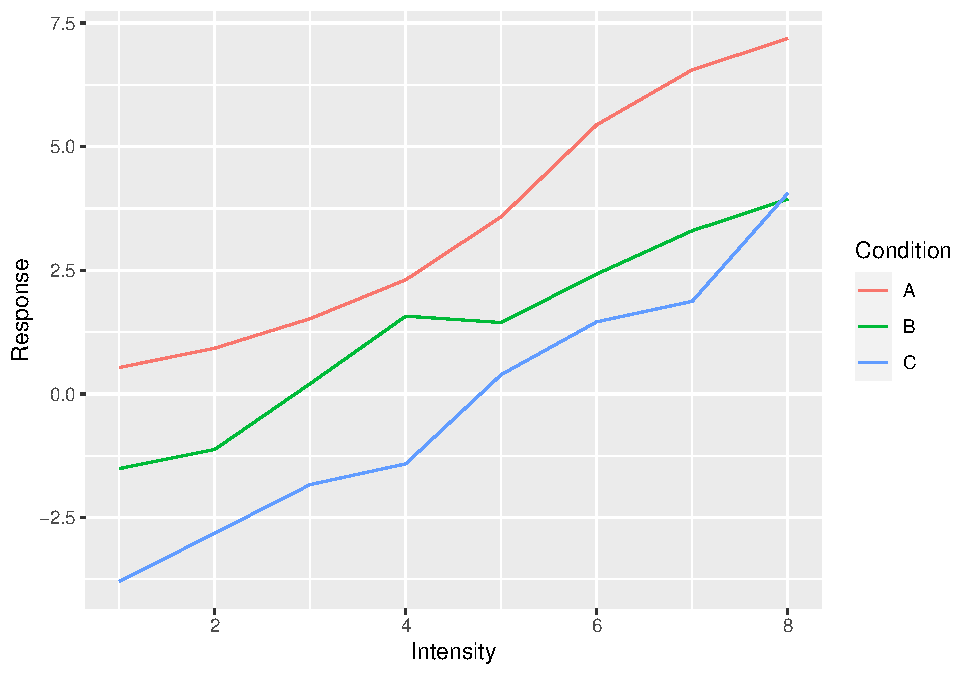
\includegraphics{data-analysis-using-r-for-psychology_files/figure-latex/unnamed-chunk-80-1.pdf}

As I already wrote, technically, we only thing you need to define is aesthetics, so let us not add anything to the plot (drop the \texttt{+geom\_line()}).

\begin{Shaded}
\begin{Highlighting}[]
\FunctionTok{ggplot}\NormalTok{(}\AttributeTok{data=}\NormalTok{simple\_tidy\_data, }\FunctionTok{aes}\NormalTok{(}\AttributeTok{x =}\NormalTok{ Intensity, }\AttributeTok{y =}\NormalTok{ Response, }\AttributeTok{color=}\NormalTok{Condition))}
\end{Highlighting}
\end{Shaded}

\begin{center}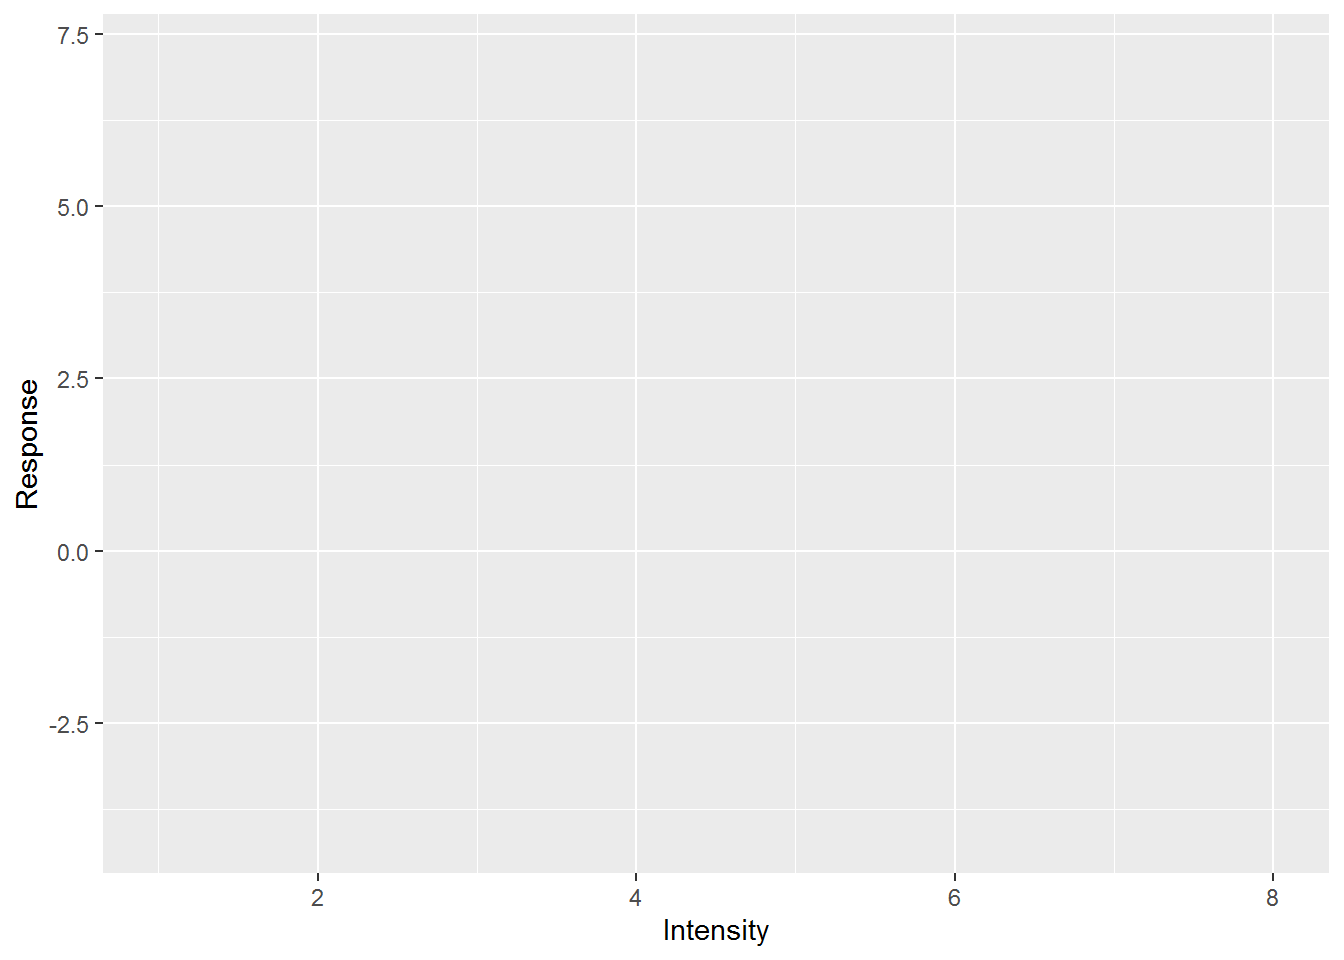
\includegraphics{data-analysis-using-r-for-psychology_files/figure-latex/unnamed-chunk-81-1} \end{center}

Told you it will look empty and yet you can see \emph{ggplot2} in action. Notice that axes are labeled and their limits are set. You cannot see the legend (they are not plotted without corresponding geometry) but it is also ready. This is because our initial call specified the most important part: how the individual variables map on various properties even before we told \emph{ggplot2} which visuals we will use to plot the data. When we specified that x-axis will represent the \texttt{Intensity}, ggplot2 figured out the range of values, so it knows \emph{where} it is going to plot whatever we decide to plot. Points, lines, bar, error bars and what not will span only that range. Same goes for other properties such as color. We wanted \emph{color} to represent the condition. Again, we may not know what exactly we will be plotting (points, lines?) or even how many different visuals we will be adding to the plot (just lines? points + lines? points + lines + linear fit?) but we do know that whatever visual we add, if it can have color, its color \emph{must} represent condition for that data point. The beauty of \emph{ggplot2} is that it analyses your data and figures out how many colors you need and is ready to apply them \emph{consistently} to all visuals you will later add. It will ensure that all points, bars, lines, etc. will have consistent coordinates scaling, color-, size-, fill-mapping that are the same across the entire plot. This may sound trivial but typically (e.g., Matlab, Matplotlib), it is \emph{your} job to make sure that all these properties match and that they represent the same value across all visual elements. And this is a pretty tedious job, particularly when you decide to change your mappings and have to redo all individual components by hand. In \emph{ggplot2}, this dissociation between mapping and visuals means you can tinker with one of them at a time. E.g. keep the visuals but change grouping or see if effect of condition is easier to see via line type, size or shape of the point? Or you can keep the mapping and see whether adding another visual will make the plot easier to understand. Note that some mapping also \emph{groups} your data, so when you use group-based visual information (e.g.~a linear regression line) it will know what data belongs together and so will perform this computation per group.

Let us see how you can keep the relationship mapping but add more visuals. Let us add both lines and points.

\begin{Shaded}
\begin{Highlighting}[]
\FunctionTok{ggplot}\NormalTok{(}\AttributeTok{data=}\NormalTok{simple\_tidy\_data, }\FunctionTok{aes}\NormalTok{(}\AttributeTok{x =}\NormalTok{ Intensity, }\AttributeTok{y =}\NormalTok{ Response, }\AttributeTok{color=}\NormalTok{Condition)) }\SpecialCharTok{+} 
  \FunctionTok{geom\_line}\NormalTok{() }\SpecialCharTok{+}
  \FunctionTok{geom\_point}\NormalTok{() }\CommentTok{\# this is new!}
\end{Highlighting}
\end{Shaded}

\begin{center}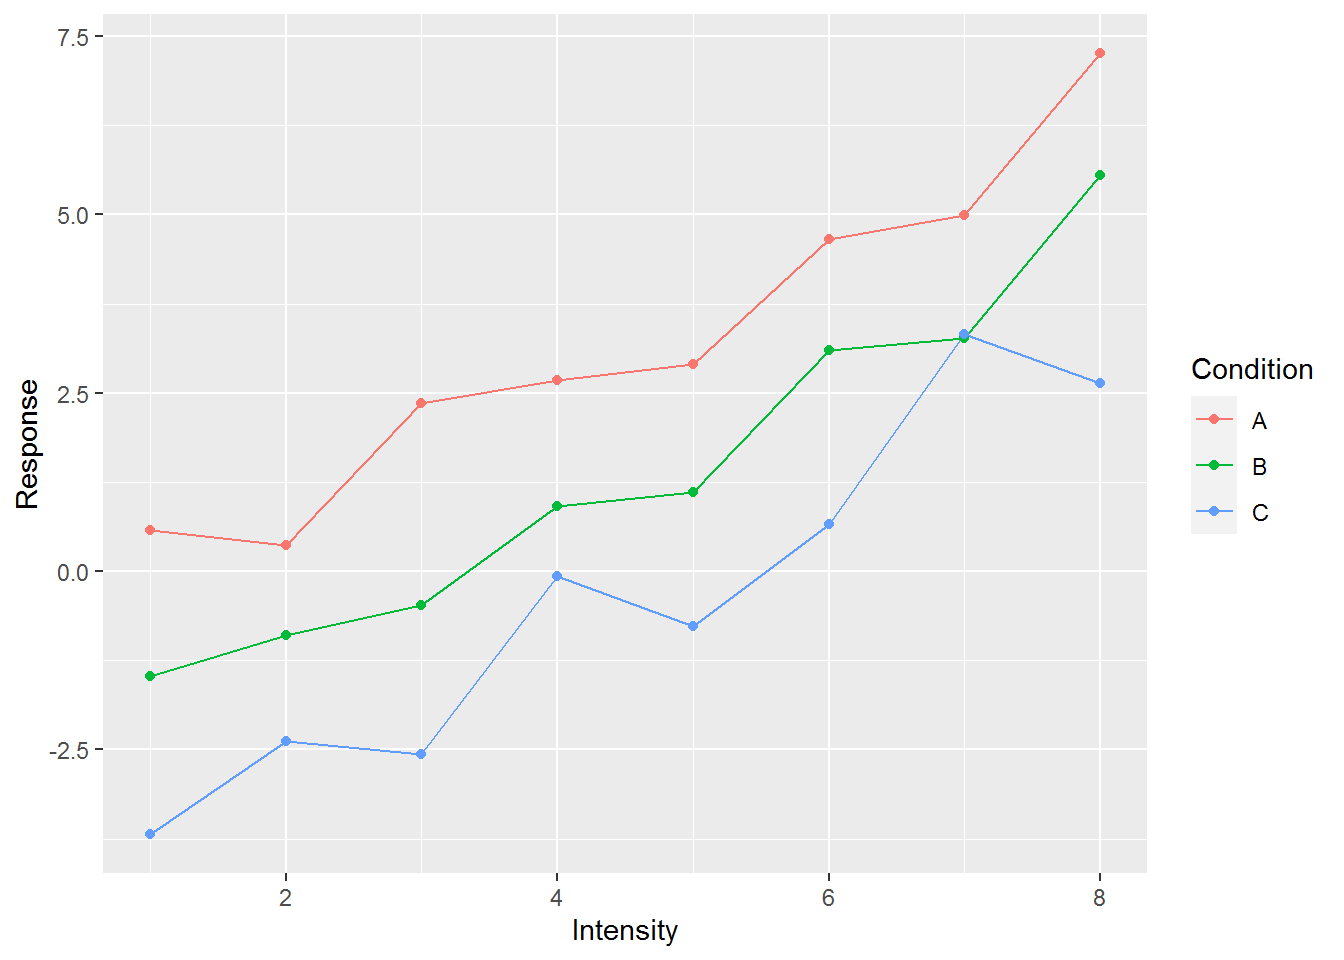
\includegraphics{data-analysis-using-r-for-psychology_files/figure-latex/unnamed-chunk-82-1} \end{center}

In the plot above, we \emph{kept} the relationship between variables and properties but said ``Oh, and throw in some points please''. And ggplot2 knows how to add the points so that they appear at proper location and in proper color. But we want more!

\begin{Shaded}
\begin{Highlighting}[]
\FunctionTok{ggplot}\NormalTok{(}\AttributeTok{data=}\NormalTok{simple\_tidy\_data, }\FunctionTok{aes}\NormalTok{(}\AttributeTok{x =}\NormalTok{ Intensity, }\AttributeTok{y =}\NormalTok{ Response, }\AttributeTok{color=}\NormalTok{Condition)) }\SpecialCharTok{+} 
  \FunctionTok{geom\_line}\NormalTok{() }\SpecialCharTok{+}
  \FunctionTok{geom\_point}\NormalTok{() }\SpecialCharTok{+}
  \CommentTok{\# a linear regression over all dots in the group}
  \FunctionTok{geom\_smooth}\NormalTok{(}\AttributeTok{method=}\StringTok{"lm"}\NormalTok{, }\AttributeTok{formula =}\NormalTok{ y }\SpecialCharTok{\textasciitilde{}}\NormalTok{ x, }\AttributeTok{se=}\ConstantTok{FALSE}\NormalTok{, }\AttributeTok{linetype=}\StringTok{"dashed"}\NormalTok{) }
\end{Highlighting}
\end{Shaded}

\begin{center}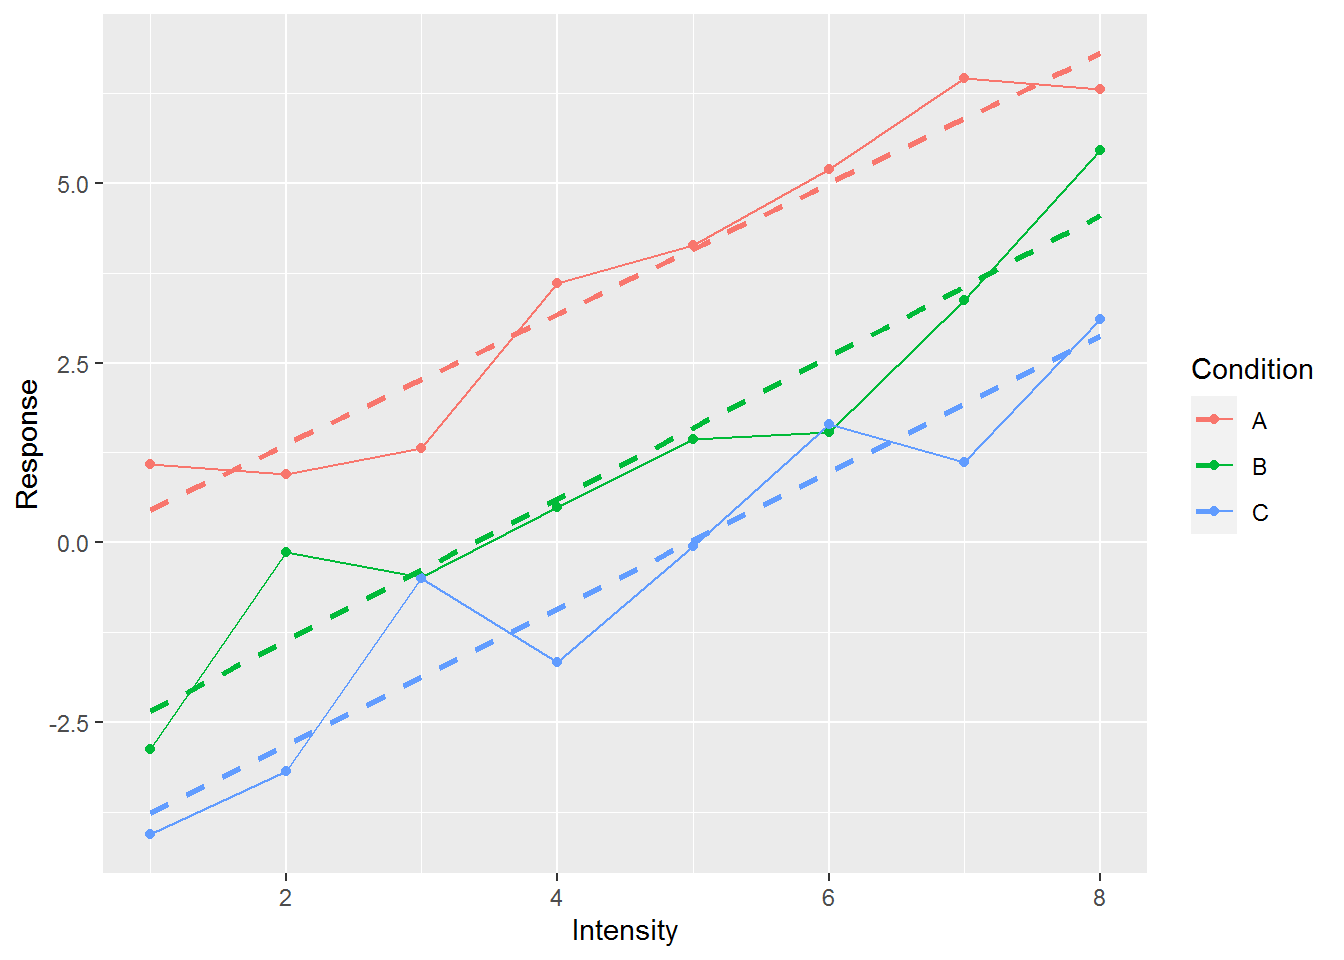
\includegraphics{data-analysis-using-r-for-psychology_files/figure-latex/unnamed-chunk-83-1} \end{center}

Now we added a linear regression line that helps us to better see the relationship between \texttt{Intensity} and \texttt{Response}. Again, we simply wished for another visual to be added (\texttt{method="lm"} means that we wanted to average data via linear regression with \texttt{formula\ =\ y\ \textasciitilde{}\ x} meaning that we regress y-axis on x-axis with no further covariates, \texttt{se=FALSE} means no standard error stripe, \texttt{linetype="dashed"} just makes it easier to distinguish from the solid data line).

Or, we can keep the \emph{visuals} but see whether changing \emph{mapping} would make it more informative (we need to specify \texttt{group=Intensity} as continuous data is not grouped automatically).

\begin{Shaded}
\begin{Highlighting}[]
\FunctionTok{ggplot}\NormalTok{(}\AttributeTok{data=}\NormalTok{simple\_tidy\_data, }\FunctionTok{aes}\NormalTok{(}\AttributeTok{x =}\NormalTok{ Condition, }\AttributeTok{y =}\NormalTok{ Response, }\AttributeTok{color=}\NormalTok{Intensity, }\AttributeTok{group=}\NormalTok{Intensity)) }\SpecialCharTok{+} 
  \FunctionTok{geom\_line}\NormalTok{() }\SpecialCharTok{+}
  \FunctionTok{geom\_point}\NormalTok{() }\SpecialCharTok{+}
  \FunctionTok{geom\_smooth}\NormalTok{(}\AttributeTok{method=}\StringTok{"lm"}\NormalTok{, }\AttributeTok{se=}\ConstantTok{FALSE}\NormalTok{,  }\AttributeTok{formula =}\NormalTok{ y }\SpecialCharTok{\textasciitilde{}}\NormalTok{ x, }\AttributeTok{linetype=}\StringTok{"dashed"}\NormalTok{)}
\end{Highlighting}
\end{Shaded}

\begin{center}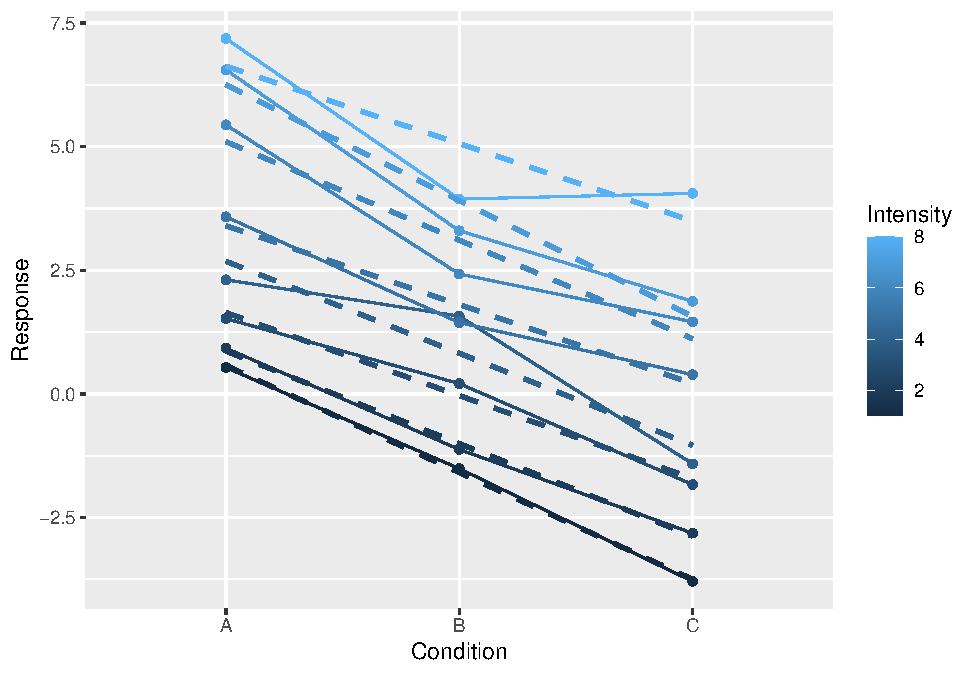
\includegraphics{data-analysis-using-r-for-psychology_files/figure-latex/unnamed-chunk-84-1} \end{center}

Or, we can check whether splitting into several plots helps.

\begin{Shaded}
\begin{Highlighting}[]
\FunctionTok{ggplot}\NormalTok{(}\AttributeTok{data=}\NormalTok{simple\_tidy\_data, }\FunctionTok{aes}\NormalTok{(}\AttributeTok{x =}\NormalTok{ Intensity, }\AttributeTok{y =}\NormalTok{ Response, }\AttributeTok{color=}\NormalTok{Condition)) }\SpecialCharTok{+} 
  \FunctionTok{geom\_line}\NormalTok{() }\SpecialCharTok{+}
  \FunctionTok{geom\_point}\NormalTok{() }\SpecialCharTok{+}
  \FunctionTok{geom\_smooth}\NormalTok{(}\AttributeTok{method=}\StringTok{"lm"}\NormalTok{, }\AttributeTok{formula =}\NormalTok{ y }\SpecialCharTok{\textasciitilde{}}\NormalTok{ x, }\AttributeTok{se=}\ConstantTok{FALSE}\NormalTok{, }\AttributeTok{linetype=}\StringTok{"dashed"}\NormalTok{) }\SpecialCharTok{+}
  \FunctionTok{facet\_grid}\NormalTok{(. }\SpecialCharTok{\textasciitilde{}}\NormalTok{ Condition) }\CommentTok{\# makes a separate subplot for each group}
\end{Highlighting}
\end{Shaded}

\begin{center}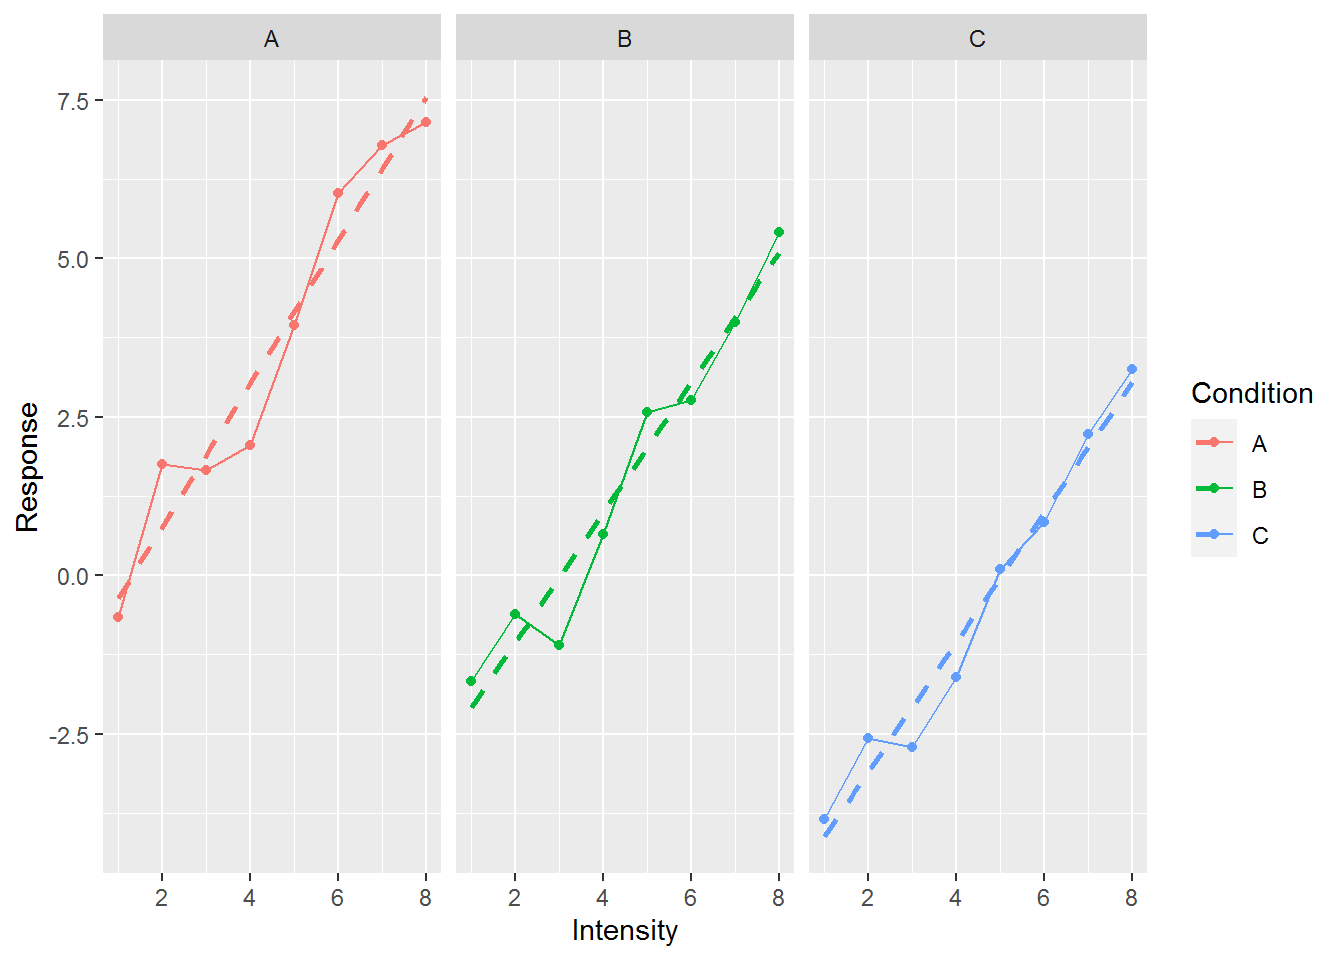
\includegraphics{data-analysis-using-r-for-psychology_files/figure-latex/unnamed-chunk-85-1} \end{center}

Again, note that all three plots live on the same scale for x- and y-axis, making them easy to compare (you fully appreciate this magic if you ever struggled with ensuring optimal and consistent scaling by hand in Matlab). I went through so many examples to stress how ggplot allows you to think about the aesthetics of variable mapping \emph{independently} of the actual visual representation (and vice versa). So now lets us explore \emph{ggplot2} by doing exercises.

I recommend using \href{https://ggplot2.tidyverse.org/}{ggplot2 reference page} and \href{https://github.com/rstudio/cheatsheets/raw/master/data-visualization-2.1.pdf}{cheatsheet} when you are doing the exercises.

\hypertarget{auto-efficiency-continuous-x-axis}{%
\section{Auto efficiency: continuous x-axis}\label{auto-efficiency-continuous-x-axis}}

We start by visualizing how car efficiency, measured as miles-per-gallon, is affected by various factors such as production year, size of the engine, type of transmission, etc. The data is in table \href{https://ggplot2.tidyverse.org/reference/mpg.html}{mpg}, which is part of the \emph{ggplot2} package. Thus, you need to first \protect\hyperlink{library}{import} the library and then load the table via \protect\hyperlink{data}{data()} function. Take a look at the \href{https://ggplot2.tidyverse.org/reference/mpg.html}{table description} to familiarize yourself with the variables.

First, let us look at the relationship between car efficiency in the city cycle (\texttt{cty}), engine displacement (\texttt{displ}), and drive train type (\texttt{drv}) using color points. Reminder, the call should look as

\begin{verbatim}
[ggplot2](https://ggplot2.tidyverse.org/reference/ggplot.html)(data_table_name, [aes](https://ggplot2.tidyverse.org/reference/aes.html)(x = var1, y = var2, color = var3, shape = var4, ...)) + 
  geom_primitive1() + 
  geom_primitive2() +
  ...
\end{verbatim}

Think about which variables are mapped on each axes and which is best depicted as color.

Do exercise 1.

Do you see any clear dependence? Let us try to making it more evident by adding \href{https://ggplot2.tidyverse.org/reference/geom_smooth.html}{geom\_smooth} geometric primitive.

Do exercise 2.

Both engine size (displacement) and drive train have a clear effect on car efficiency. Let us visualize the number of cylinders (\texttt{cyl}) as well. Including it by mapping it on the \emph{size} of geometry.

Do exercise 3.

Currently, we are mixing together cars produced at different times. Let us visually separate them by turning each year into a subplot via \href{https://ggplot2.tidyverse.org/reference/facet_wrap.html}{facet\_wrap} function.

Do exercise 4.

The dependence you plotted does not look linear but instead is saturating at certain low level of efficiency. This sort of dependencies could be easier to see on a logarithmic scale. See functions for different \href{https://ggplot2.tidyverse.org/reference/scale_continuous.html}{scales} and use logarithmic scaling for y-axis.

Do exercise 5.

Note that by now we managed to include \emph{five} variables into our plots. We can continue this by including transmission or fuel type but that would be pushing it, as too many variables can make a plot confusing and cryptic. Instead, let us make it prettier by using more meaningful axes labels (\texttt{xlab()}, \texttt{ylab()} functions) and adding a plot title (\href{https://ggplot2.tidyverse.org/reference/labs.html}{labs}).

Do exercise 6.

\hypertarget{auto-efficiency-discrete-x-axis}{%
\section{Auto efficiency: discrete x-axis}\label{auto-efficiency-discrete-x-axis}}

The previous section use a continuous engine displacement variable for x-axis (at least that is my assumption on how you mapped the variables). Frequently, you need to plot data for discrete groups: experimental groups, conditions, treatments, etc. Let us practice on the same \href{https://ggplot2.tidyverse.org/reference/mpg.html}{mpg} data set but visualize relationship between the drive train (\texttt{drv}) and highway cycle efficiency (\texttt{hwy}). Start by using point as visuals.

Do exercise 7.

One problem with the plot is that all points are plotted at the same x-axis location. This means that if two points share the location, they overlap and appear as just one dot. This makes it hard to understand the density: one point can mean one point, or two, or a hundred. A better way to plot such data is by using \href{https://ggplot2.tidyverse.org/reference/geom_boxplot.html}{box} or {]}violin{]}(\url{https://ggplot2.tidyverse.org/reference/geom_violin.html}) plots. Experiment by using them instead of points.

Do exercise 8.

Again, let's up the ante and split plots via both number of cylinders and year of manufacturing. Use \href{https://ggplot2.tidyverse.org/reference/facet_grid.html}{facet\_grid} function to generate grid of plots.

Do exercise 9.

Let us again improve our presentation by using better axes labels and figure title.

Do exercise 10.

\hypertarget{mammals-sleep-single-variable}{%
\section{Mammals sleep: single variable}\label{mammals-sleep-single-variable}}

Now lets us work on plotting a distribution for a single variable using \href{https://ggplot2.tidyverse.org/reference/msleep.html}{mammals sleep dataset}. For this, you need to map \texttt{sleep\_total} variable on x-axis and plot a \href{https://ggplot2.tidyverse.org/reference/geom_histogram.html}{histogram}. Explore the available options, in particular \texttt{bins} that determines the bins number and, therefore, their size. Note that there is no ``correct'' number of bins to use. \emph{ggplot2} defaults to 30 but a small sample would be probably better served with fewer bins and, vice versa, with a large data set you can afford hundred of bins.

Do exercise 11.

Using a histogram gives you exact counts per each bin. However, the appearance may change quite dramatically if you would use fewer or more bins. An alternative way to represent the same information is via \href{https://ggplot2.tidyverse.org/reference/geom_density.html}{smoothed density estimates}. They use a sliding window and compute an estimate at each point but also include points \emph{around} it and weight them according to a kernel (e.g.~a Gaussian one). This makes the plot look smoother and will mask sudden jumps in density (counts) as you, effectively, average over many bins. Whether this approach is better for visualizing data depends on the sample you have and message you are trying to get across. It is always worth checking both (just like it is worth checking different number of bins in histogram) to see which way is the best for your specific case.

Do exercise 12.

Let us return to using histograms and plot a distribution per \texttt{vore} variable (it is \texttt{carnivore}, \texttt{omnivore}, \texttt{herbivore}, or \texttt{NA}). You can map it on the \texttt{fill} color of the histogram, so that each \emph{vore} kind will be binned separately.

Do exercise 13.

The plot may look confusing because by default \emph{ggplot2} colors values for each group differently but stacks all of them together to produce the total histogram counts. One way to disentangle the individual histograms is via \href{https://ggplot2.tidyverse.org/reference/facet_grid.html}{facet\_grid} function. Use it to plot \texttt{vore} distribution in separate rows.

Do exercise 14.

That did the trick but there is an alternative way to plot individual distributions on the same plot by setting \texttt{position} argument of geom\_histogram to \texttt{"identity"} (it is \texttt{"stack"} by default).

Do exercise 15.

Hmm, shouldn't we have more carnivores, what is going on? Opacity is the answer. A bar ``in front'' occludes any bars that are ``behind'' it. Go back to the exercise and fix that by specifying \texttt{alpha} argument that controls transparency. It is \texttt{1} (completely opaque) by default and can go down to \texttt{0} (fully transparent as in ``invisible''), so see which intermediate value works the best.

\hypertarget{mapping-for-all-visuals-versus-just-one-visual}{%
\section{Mapping for all visuals versus just one visual}\label{mapping-for-all-visuals-versus-just-one-visual}}

In the previous exercise, you assigned a constant value to \texttt{alpha} (transparency) argument. You could do this in \emph{two} places, inside of either \texttt{ggplot()} or \texttt{geom\_histogram()} call. In the former case, you would have set \texttt{alpha} level for \emph{all} geometric primitives on the plot, whereas in the latter you do it only for the histogram. To better see the difference, reuse your code for plotting city cycle efficiency versus engine size (should be exercise \#6) and set \texttt{alpha} either for all visuals (in \texttt{ggplot2}) or in some visuals (e.g.~only for points) to see the difference.

Do exercise 16.

\hypertarget{mapping-on-variables-versus-constants}{%
\section{Mapping on variables versus constants}\label{mapping-on-variables-versus-constants}}

In the previous exercise, you assigned a constant value to \texttt{alpha} (transparency) argument. However, transparency is just a property just like \texttt{x}, \texttt{color}, or \texttt{size}. Thus, there are \emph{two} ways you can use them:

\begin{itemize}
\tightlist
\item
  \emph{inside} \texttt{aes(x=column)}, where \texttt{column} is column in the table you supplied via \texttt{data=}
\item
  \emph{outside} of \texttt{aes} by stating \texttt{x=value}, where value is some constant value or a variable \emph{that is not in the table}.
\end{itemize}

Test this but setting the \texttt{size} in the previous plot to a constant outside of aesthetics or to a variable inside of it.

Do exercise 17.

\hypertarget{themes}{%
\section{Themes}\label{themes}}

Finally, if you are not a fan of the way the plots look, you can quickly modify this by using some other theme. You can define it yourself (there are lots of options you can specify for your \href{https://ggplot2.tidyverse.org/reference/theme.html}{theme}) or can use one of the \href{https://ggplot2.tidyverse.org/reference/ggtheme.html}{ready-mades}. Explore the latter option, find the one you like the best.

Do exercise 18.

\hypertarget{you-aint-seen-nothing-yet}{%
\section{You ain't seen nothing yet}\label{you-aint-seen-nothing-yet}}

What you explored is just a tip of the iceberg. There are many more geometric primitive, annotations, scales, themes, etc. It will take an entire separate seminar to do \emph{ggplot2} justice. However, the basics will get you started and you can always consult reference, books (see below), or me once you need more.

\hypertarget{further-reading}{%
\section{Further reading}\label{further-reading}}

If plotting data is part of your daily routine, I recommend reading \href{https://ggplot2-book.org/}{ggplot2 book}. It gives you an in-depth view of the package and goes through many possibilities that it offers. You may need all of them but I find useful to know that they exists (who knows, I might need them one day). Another book worth reading is \href{https://kieranhealy.org/publications/dataviz/}{Data Visualization: A Practical Introduction.} by Kieran Healy.

\hypertarget{extending-ggplot2}{%
\section{Extending ggplot2}\label{extending-ggplot2}}

There are 80 (as of 19.11.2020) extensions that you find at \href{https://exts.ggplot2.tidyverse.org/gallery/}{ggplot2 website}. They add more ways to plot your data, more themes, animated plots, etc. If you feel that \emph{ggplot2} does not have the geometric primitives you need, take a look at the gallery and, most likely, you will find something that fits your bill.

One package that is \emph{not} in the gallery is \href{https://patchwork.data-imaginist.com/}{patchwork}. It was created ``to make it ridiculously simple to combine separate ggplots into the same graphic''. It is a bold promise but authors do make good on it. It is probably the easiest way to combine multiple plots but you can also consider \href{https://github.com/wilkelab/cowplot}{cowplot} and \href{https://cran.r-project.org/web/packages/gridExtra/index.html}{gridExtra} packages.

\hypertarget{ggplot2-cannot-do-everything}{%
\section{ggplot2 cannot do everything}\label{ggplot2-cannot-do-everything}}

There are many different plotting routines and packages for R but I would recommend to use \emph{ggplot2} as your main tool. However, that does not mean that it must be your only tool, after all, CRAN is brimming with packages. In particular, \emph{ggplot2} is built for plotting data from a single tidy table, meaning it is less optimal for plotting data in other cases. E.g., you can use it to combine information from several tables in one plot but things become less automatic and consistent. Similarly, you can plot data which is stored in non-tidy tables or even in individual vectors but that makes it less intuitive and more convoluted. No package can do everything and \emph{ggplot2} is no exception.

\hypertarget{seminar05}{%
\chapter{Functions and pipes}\label{seminar05}}

In this seminar, you will learn about \emph{functions} in R, as they are the second most important concept in R and are everywhere (just like vectors). You will also learn how to \emph{pipe} your computation through series of functions without creating a mess of temporary variables or nested calls. Don't forget to download the \href{notebooks/Seminar\%2005\%20-\%20functions.Rmd}{notebook}.

\hypertarget{functions}{%
\section{Functions}\label{functions}}

In the previous seminars, you have learned that you can store information in variables --- ``boxes with slots'' --- as \protect\hyperlink{vectors}{vectors} or as \protect\hyperlink{ux5cux23tables}{tables} (bundles of vectors of equal length). To use these stored values for computation you need functions. In programming, function is an \emph{isolated} code with a name that receives some input, performs some action on them, and, optionally, returns a value\footnote{Function that does not return a value, probably, generates its output to a console, external file, etc. There is little point in running a function that does not affect the world.}. The concepts of functions comes from mathematics, so it might be easier to understand them using R implementation of mathematical functions. For example, you may remember sinus function from trigonometry. It is typically abbreviated as \texttt{sin}, it takes a numeric value of angle (in radians) as its \emph{input} and returns a corresponding value between -1 and 1: \(sin(0) = 0\), \(sin(\pi/2) = 1\), etc. (this is its \emph{output}).

\begin{center}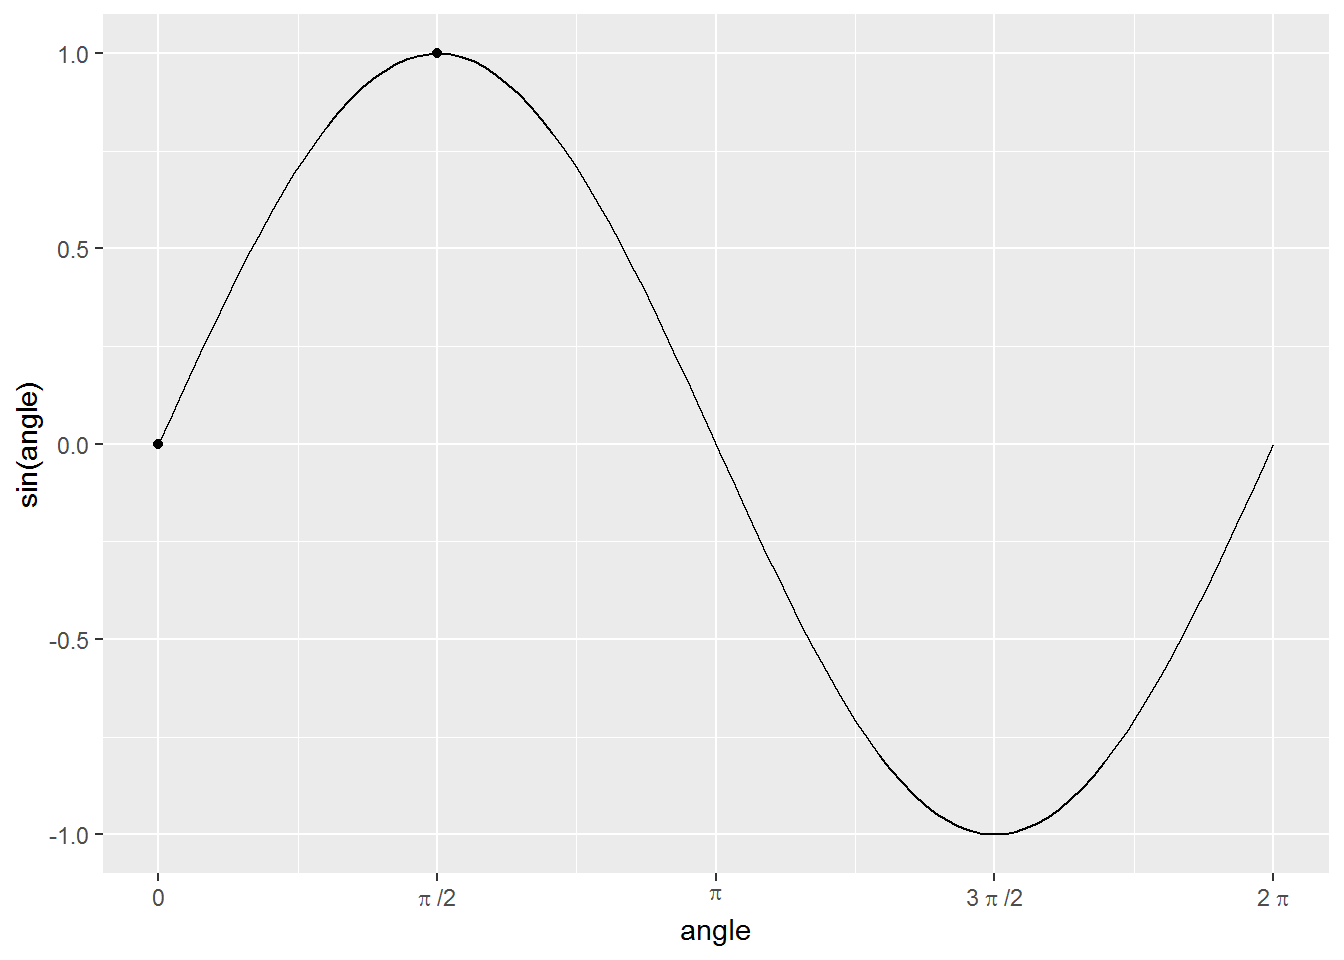
\includegraphics{data-analysis-using-r-for-psychology_files/figure-latex/unnamed-chunk-87-1} \end{center}

In R, you write a function using the following template\footnote{Did you spot the assignment \texttt{\textless{}-} operator? Yes, you are storing a function code in a variable. So when you call this function by name, you are asking to run the code stored inside that variable.}

\begin{Shaded}
\begin{Highlighting}[]
\NormalTok{name\_of\_the\_function }\OtherTok{\textless{}{-}} \ControlFlowTok{function}\NormalTok{(parameter1, parameter2, parameter3, ...)\{}
\NormalTok{  ...some code that computes the value...}
  \FunctionTok{return}\NormalTok{(value);}
\NormalTok{\}}
\end{Highlighting}
\end{Shaded}

Thus, \texttt{sin} function with a single parameter \texttt{angle} would look something like this

\begin{Shaded}
\begin{Highlighting}[]
\NormalTok{sin }\OtherTok{\textless{}{-}} \ControlFlowTok{function}\NormalTok{(angle)\{}
\NormalTok{  ...some math that actually computes sin\_of\_angle using value of angle parameter ...}
  \FunctionTok{return}\NormalTok{(sin\_of\_angle);}
\NormalTok{\}}
\end{Highlighting}
\end{Shaded}

Once we have the function, we can use it by \emph{calling} it. You simply write \texttt{sin(0)} and get the answer!

\begin{Shaded}
\begin{Highlighting}[]
\FunctionTok{sin}\NormalTok{(}\DecValTok{0}\NormalTok{)}
\end{Highlighting}
\end{Shaded}

\begin{verbatim}
## [1] 0
\end{verbatim}

As you hopefully remember, everything is a vector, so instead of using a scalar \texttt{0} (merely a vector of length of one) you can write and apply this function to (compute sinus for) every element in the vector.

\begin{Shaded}
\begin{Highlighting}[]
\FunctionTok{sin}\NormalTok{(}\FunctionTok{seq}\NormalTok{(}\DecValTok{0}\NormalTok{, }\FloatTok{3.141593}\NormalTok{, }\AttributeTok{length.out =} \DecValTok{5}\NormalTok{))}
\end{Highlighting}
\end{Shaded}

\begin{verbatim}
## [1]  0.000000e+00  7.071068e-01  1.000000e+00  7.071066e-01 -3.464102e-07
\end{verbatim}

You can think of functions parameters as local function variables those values are set before the function is called. A function can have any number of parameters, including zero\footnote{This, probably, means that the function always does the same thing or a random thing and you cannot influence this.}, one, or many parameters. For example, an arctangent \href{https://stat.ethz.ch/R-manual/R-devel/library/base/html/Trig.html}{atan2} function takes 2D coordinates (\texttt{y} and \texttt{x}, in that order!) and returns a corresponding angle in radians (relative to \texttt{(0,\ 0)} point).

\begin{Shaded}
\begin{Highlighting}[]
\FunctionTok{atan2}\NormalTok{(}\FunctionTok{c}\NormalTok{(}\DecValTok{0}\NormalTok{, }\DecValTok{1}\NormalTok{), }\FunctionTok{c}\NormalTok{(}\DecValTok{1}\NormalTok{, }\DecValTok{1}\NormalTok{))}
\end{Highlighting}
\end{Shaded}

\begin{verbatim}
## [1] 0.0000000 0.7853982
\end{verbatim}

A definition of this function would look something like this

\begin{Shaded}
\begin{Highlighting}[]
\NormalTok{atan2 }\OtherTok{\textless{}{-}} \ControlFlowTok{function}\NormalTok{(y, x)\{}
\NormalTok{  ...magic that uses values of y and x parameters...}
\NormalTok{  ...to compute the angle\_in\_rad value...}
  \FunctionTok{return}\NormalTok{(angle\_in\_rad);}
\NormalTok{\}}
\end{Highlighting}
\end{Shaded}

Do exercise 1.

\hypertarget{writing-a-function}{%
\section{Writing a function}\label{writing-a-function}}

Let us start practicing computing things in R and writing functions at the same time. We will begin by implementing a very simple function that doubles a given number. We will write this function in steps. First, think about how you would name\footnote{\texttt{double\_or\_nothing}?} this function (meaningful names are your path to readable and usable code!) and how many parameters it will have. Write the all the definition of the function but without any code inside of wiggle brackets (so, no actual computation or a return statement at the end of it).

Do exercise 2.1

Next, think about the code that does \emph{double-the-value} computation based on the parameter. This is the code that will eventually go inside of the wiggly brackets. Write that code in exercise 2.2 and test it by creating a variable with the same name as your parameter inside the function. E.g., if my parameter name is \texttt{the\_number}, I would test it as

\begin{Shaded}
\begin{Highlighting}[]
\NormalTok{the\_number }\OtherTok{\textless{}{-}} \DecValTok{1}
\NormalTok{...my code to double the value usign the\_number variable...}
\end{Highlighting}
\end{Shaded}

Do exercise 2.2

By now you have your formal function definition (exercise 2.1) and the actual code that should go inside (exercise 2.2). Now, we just need to combine them by putting the code inside the function and \emph{returning} the value. You can do this two ways:

\begin{enumerate}
\def\labelenumi{\arabic{enumi})}
\tightlist
\item
  you can store the results of the computation in a separate local variable and then return that variable,
\item
  return the results of the computation directly
\end{enumerate}

\begin{verbatim}
# 1) first store in a local variable, then return it
  result <- ...some computation you perform...
  return(result);

# 2) returning results of computation directly
  return(...some computation you perform...);
\end{verbatim}

Do it \emph{both} ways in exercises 2.3 and 2.4. Call the function to test that it works.

Do exercise 2.3 and 2.4

More practice is good, so write a function that converts an angle in \emph{degrees} to \emph{radians}. The formula is
\[rad = \frac{deg \cdot \pi}{180}\]
Decide whether you want to a have an intermediate local variable inside the function or to return the results of the computation directly.

Do exercise 3

\hypertarget{scopes-global-versus-local-variables}{%
\section{Scopes: Global versus Local variables}\label{scopes-global-versus-local-variables}}

I suggested that you use a variable to store the results of double-it-up computation before returning it. But why did I call it \emph{local}? This is because each function has it own \emph{scope} (environment with variables and functions) that is (mostly) independent from the scope of the global script. Unfortunately, environment scopes in R are different and more complicated than those in other programming languages, such Python, C/C++, or Java, so pay attention and be careful in the future.

The \emph{global} scope/environment is the environment for the code \emph{outside} of functions. All \emph{global} variables and functions, the ones that you define in the code \emph{outside} of functions (typing in the console, running scripts, chunks of code in notebooks, etc.), live where. You can see what you have in the global scope at any time by looking at \emph{Environment} tab (note the \emph{Global Environment} tag).

\begin{center}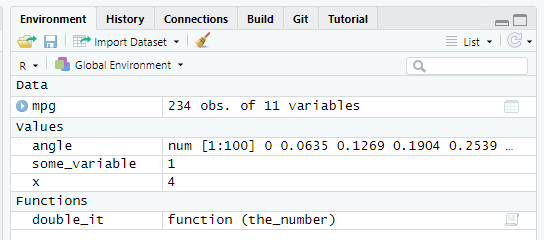
\includegraphics[width=0.7\linewidth]{images/environment-tab} \end{center}

In my case, it has one table (\texttt{mpg}, all tables go under \emph{Data}), three vectors (\texttt{angle}, \texttt{some\_variable}, and \texttt{x}, all vectors go under \texttt{Values}), and an example function from exercise \#2 that I created (\texttt{double\_it}, all functions go under \emph{Functions}, makes sense). However, it has no access to parameters of the functions and variables that you define inside these function. When you run a function, it has it own scope/environment that includes \emph{parameters} of the function (e.g., \texttt{the\_number} for my \texttt{double\_it} function and the value it was assigned during the call), any \emph{local} variables you create inside that function (e.g., \texttt{result\ \textless{}-\ ...some\ computation\ you\ perform...} creates such local variable), and a \textbf{copy(!)} of all \emph{global} variables. In the code below, take a look at the comments that specify the accessibility of variables between global script and functions (ignore \href{https://glue.tidyverse.org/reference/glue.html}{glue} for a moment, it \emph{glues} variable value into the text, so I use it to make printouts easier to trace)\footnote{These rules --- a \textbf{copy} of a global scope is accessible inside a function but function scope is inaccessible from outside --- should be how \emph{you} write your code. However, R's motto is ``anything is possible'', so be aware that \emph{other people} may not respect these rules. This should not be an issue most of the time but if you are curious how R can let you break all rules of good responsible programming and do totally crazy things, read \href{https://adv-r.hadley.nz/}{Advanced R} book by Hadley Wickham. However, it is really \textbf{advanced}, aimed primarily at programmers who develop R and packages, not at scientists who use them.}

\begin{Shaded}
\begin{Highlighting}[]
\CommentTok{\# this is a GLOBAL variable}
\NormalTok{global\_variable }\OtherTok{\textless{}{-}} \DecValTok{1}

\NormalTok{i\_am\_test\_function }\OtherTok{\textless{}{-}} \ControlFlowTok{function}\NormalTok{(parameter)\{}
  \CommentTok{\# parameter live is a local function scope}
  \CommentTok{\# its values are set when you call a function}
  \FunctionTok{print}\NormalTok{(}\FunctionTok{glue}\NormalTok{(}\StringTok{"  parameter inside the function: \{parameter\}"}\NormalTok{))}
  
  \CommentTok{\# local variable created inside the function}
  \CommentTok{\# it is invisible from outside}
\NormalTok{  local\_variable }\OtherTok{\textless{}{-}} \DecValTok{2}
  \FunctionTok{print}\NormalTok{(}\FunctionTok{glue}\NormalTok{(}\StringTok{"  local\_variable inside the function: \{local\_variable\}"}\NormalTok{))}
  
  \CommentTok{\# here, a\_global\_variable is a LOCAL COPY of the the global variable}
  \CommentTok{\# of the same name. You can use this COPY}
  \FunctionTok{print}\NormalTok{(}\FunctionTok{glue}\NormalTok{(}\StringTok{"  COPY of global\_variable inside the function: \{global\_variable\}"}\NormalTok{))}
  
  \CommentTok{\# you can modify the LOCAL COPY but that won\textquotesingle{}t affect the original!}
\NormalTok{  global\_variable }\OtherTok{\textless{}{-}} \DecValTok{3}
  \FunctionTok{print}\NormalTok{(}\FunctionTok{glue}\NormalTok{(}\StringTok{"  CHANGED COPY of global\_variable inside the function: \{global\_variable\}"}\NormalTok{))}
\NormalTok{\}}

\FunctionTok{print}\NormalTok{(}\FunctionTok{glue}\NormalTok{(}\StringTok{"global\_variable before the function call: \{global\_variable\}"}\NormalTok{))}
\end{Highlighting}
\end{Shaded}

\begin{verbatim}
## global_variable before the function call: 1
\end{verbatim}

\begin{Shaded}
\begin{Highlighting}[]
\FunctionTok{i\_am\_test\_function}\NormalTok{(}\DecValTok{5}\NormalTok{)}
\end{Highlighting}
\end{Shaded}

\begin{verbatim}
##   parameter inside the function: 5
##   local_variable inside the function: 2
##   COPY of global_variable inside the function: 1
##   CHANGED COPY of global_variable inside the function: 3
\end{verbatim}

\begin{Shaded}
\begin{Highlighting}[]
\CommentTok{\# the variable outside is unchanged because we modify its COPY, not the variable itself}
\FunctionTok{print}\NormalTok{(}\FunctionTok{glue}\NormalTok{(}\StringTok{"UNCHANGED global\_variable after the function call: \{global\_variable\}"}\NormalTok{))}
\end{Highlighting}
\end{Shaded}

\begin{verbatim}
## UNCHANGED global_variable after the function call: 1
\end{verbatim}

Do exercise 4 to build understanding of scopes.

\hypertarget{function-with-two-parameters}{%
\section{Function with two parameters}\label{function-with-two-parameters}}

Let us write a function that takes \emph{two} parameters --- \texttt{x} and \texttt{y} --- and computes \emph{radius} (distance from \texttt{(0,0)} to \texttt{(x,\ y)})\footnote{This function is complementary to \texttt{atan2()}, as two of them allow transformation of coordinates from cartesian to polar coordinate system}. The formula is
\[R = \sqrt{x^2 + y^2}\]
This is very similar to exercises 2 and 3, with number of parameters being the only difference.

Do exercise 5.

\hypertarget{table-as-a-parameter}{%
\section{Table as a parameter}\label{table-as-a-parameter}}

So far, we passed only vectors (a.k.a. values) to functions but you can pass any object including tables\footnote{And even functions themselves, not just what they computed! This is part of \emph{functional programming} you will learn about later.}. Let us use \href{https://ggplot2.tidyverse.org/reference/mpg.html}{mpg} table from the \emph{ggplot2} package. Write a function that takes a table as a \emph{parameter}. This mean that function should not assume that table with this name exists in the global environment. Do not use \texttt{mpg} as a parameter name (makes is confusing), call it something else. The function should compute and return average miles-per-gallon efficiency based on city \texttt{cty} and highway \texttt{hwy} test cycles. Do it in \emph{two} ways. First, compute and return \emph{a vector} based on the table passed as parameter. Second, do the same computation but add the result \emph{to the table function received as a parameter} (call the column \texttt{avg\_mpg}) and return the entire table.

Do exercise 6.

Let us write another function that computes \href{https://stat.ethz.ch/R-manual/R-devel/library/base/html/mean.html}{mean} efficiency for a particular cycle, either city or highway. For this, the function will take \emph{two} parameters: 1) the table itself and 2) a string (text variable) with the name of the column. You can then use it to access the column via \protect\hyperlink{get-single-column}{double square brackets} notation. To summarize, your function takes 1) a table and 2) a string with a column name and returns a single number (mean for the specified column). E.g.

\begin{Shaded}
\begin{Highlighting}[]
\FunctionTok{average\_efficiency}\NormalTok{(mpg, }\StringTok{"cty"}\NormalTok{) }\CommentTok{\# should return 16.85897}
\end{Highlighting}
\end{Shaded}

Do exercise 7.

\hypertarget{nested-calls}{%
\section{Nested calls}\label{nested-calls}}

What if you need to call several functions in a single chain to compute the result? Think about the function from exercise \#3 that converts degree to radians. Its most likely usage scenario is to convert degrees to radians and use that to compute sinus (or some other trigonometric function). There are different ways you can do this. For example, you can store the angle in radians in some temporary variable (e.g., \texttt{angle\_in\_radians}) and then pass it to sinus function during the next call.

\begin{Shaded}
\begin{Highlighting}[]
\NormalTok{angle\_in\_radians }\OtherTok{\textless{}{-}} \FunctionTok{deg2rad}\NormalTok{(}\DecValTok{90}\NormalTok{) }\CommentTok{\# functoin returns 1.570796, this value is stored in angle\_in\_radians}
\FunctionTok{sin}\NormalTok{(angle\_in\_radians) }\CommentTok{\# returns 1}
\end{Highlighting}
\end{Shaded}

Alternatively, you can use the value returned by \texttt{deg2rad()} directly as a parameter for function \texttt{sin()}

\begin{Shaded}
\begin{Highlighting}[]
\FunctionTok{sin}\NormalTok{(}\FunctionTok{deg2rad}\NormalTok{(}\DecValTok{90}\NormalTok{)) }\CommentTok{\# returns 1}
\end{Highlighting}
\end{Shaded}

In this case, the computation proceeds in an \emph{inside-out} order: The innermost function gets computed first, the function that uses its return value is next, etc. Kind of like assembling a Russian doll: you start with an innermost, put it inside a slightly bigger one, now take that one put it inside the next, etc. Nesting means that you do not need to pollute you memory with temporary variables\footnote{The worst case scenario is when you use same \texttt{temp} variable for things like that, forget to initialize / change its value it properly at some point, spend half-a-day trying to understand why your code works but results don't make sense.} and make your code more expressive as nesting explicitly informs the reader that intermediate results are of no value by themselves and are not saved for later use.

Do exercise 8.

\hypertarget{piping}{%
\section{Piping}\label{piping}}

Although nesting is better than having tons of intermediate variables, lots of nesting can be mightily confusing. Tidyverse has an alternative way to chain or, in Tidyverse-speak, \href{https://magrittr.tidyverse.org/reference/pipe.html}{pipe} a computation through a series of function calls. The magic operator is \texttt{\%\textgreater{}\%} (that's the pipe) and here is how it transforms our nested call

\begin{Shaded}
\begin{Highlighting}[]
\FunctionTok{sin}\NormalTok{(}\FunctionTok{deg2rad}\NormalTok{(}\DecValTok{90}\NormalTok{)) }\CommentTok{\# returns 1}

\FunctionTok{deg2rad}\NormalTok{(}\DecValTok{90}\NormalTok{) }\SpecialCharTok{\%\textgreater{}\%} \FunctionTok{sin}\NormalTok{() }\CommentTok{\# also return 1}

\DecValTok{90} \SpecialCharTok{\%\textgreater{}\%} \FunctionTok{deg2rad}\NormalTok{() }\SpecialCharTok{\%\textgreater{}\%} \FunctionTok{sin}\NormalTok{() }\CommentTok{\# also returns 1}
\end{Highlighting}
\end{Shaded}

Do exercise 9.

All functions you worked in the exercise with had only one parameter and \texttt{single-output\ \%\textgreater{}\%\ single-input} piping is very straightforward. But what if one of the functions takes more than one parameter? By default, \texttt{\%\textgreater{}\%} puts the piped value into the \emph{first} parameter. Thus \texttt{4\ \%\textgreater{}\%\ radius(3)} is equivalent to \texttt{radius(4,\ 3)}. Although this default is very useful (the entire Tidyverse is build around this idea of piping a value into the \emph{first} parameter), sometimes you need that value as some \emph{other} parameter (e.g., when you are pre-processing the data before piping it into a statistical test, the latter typically takes \texttt{formula} as the first parameter and \texttt{data} as second). For this, you can use a special dot variable: \texttt{.}, which is a hidden\footnote{It won't show up in your Global Environment tab.} temporary variable that holds the value you are piping through via \texttt{\%\textgreater{}\%}\footnote{Yes, it is the same variable that you use over-and-over again but \texttt{magritt} package makes sure to clean it up after each call, so you are not in danger of incidentally using a value from a previous call.}. Thus,

\begin{Shaded}
\begin{Highlighting}[]
\NormalTok{z }\OtherTok{\textless{}{-}} \DecValTok{4}
\NormalTok{w }\OtherTok{\textless{}{-}} \DecValTok{3}
\NormalTok{z }\SpecialCharTok{\%\textgreater{}\%} \FunctionTok{radius}\NormalTok{(w) }\CommentTok{\# is equivalent to radius(z, w)}

\CommentTok{\# Note the dot!}
\NormalTok{z }\SpecialCharTok{\%\textgreater{}\%} \FunctionTok{radius}\NormalTok{(w, .) }\CommentTok{\# is equivalent to radius(w, z)}
\end{Highlighting}
\end{Shaded}

Note that because \texttt{.} is a variable, you can use it several times just as you can use several times any variable

\begin{Shaded}
\begin{Highlighting}[]
\DecValTok{4} \SpecialCharTok{\%\textgreater{}\%} \FunctionTok{radius}\NormalTok{(., .) }\CommentTok{\# is equivalent to radius(4, 4)}
\end{Highlighting}
\end{Shaded}

Do exercise 10.

\hypertarget{everything-is-a-function}{%
\section{Everything is a function}\label{everything-is-a-function}}

Every computation you perform in R is implemented as a function, even when using one does not look like a function call. For example, \texttt{+} addition operation is a function. Typically, you write \texttt{2\ +\ 3}, so no round brackets, no comma-separated list of parameters, it looks different. But this is just a special implementation of a function call (known as \href{http://adv-r.had.co.nz/Function-operators.html}{function operator}) that makes code more readable for humans. You can actually call \texttt{+} function the way you call a normal function by using backticks around its name.

\begin{Shaded}
\begin{Highlighting}[]
\DecValTok{2} \SpecialCharTok{+} \DecValTok{3}
\end{Highlighting}
\end{Shaded}

\begin{verbatim}
## [1] 5
\end{verbatim}

\begin{Shaded}
\begin{Highlighting}[]
\CommentTok{\# note the \textasciigrave{}backticks\textasciigrave{} around +}
\StringTok{\textasciigrave{}}\AttributeTok{+}\StringTok{\textasciigrave{}}\NormalTok{(}\DecValTok{2}\NormalTok{, }\DecValTok{3}\NormalTok{)}
\end{Highlighting}
\end{Shaded}

\begin{verbatim}
## [1] 5
\end{verbatim}

Even the assignments statement \texttt{\textless{}-} is, you've guessed it, a function

\begin{Shaded}
\begin{Highlighting}[]
\StringTok{\textasciigrave{}}\AttributeTok{\textless{}{-}}\StringTok{\textasciigrave{}}\NormalTok{(some\_variable, }\DecValTok{1}\NormalTok{)}
\NormalTok{some\_variable}
\end{Highlighting}
\end{Shaded}

\begin{verbatim}
## [1] 1
\end{verbatim}

This does not mean that you should start using operators as functions (although, if it helps to make a particular code clearer, then, why not?), merely to stress that there is only one way to program any computation in R --- as a function --- regardless of how it may appear in the code. Later on, you will learn how to \href{https://stat.ethz.ch/R-manual/R-devel/library/base/html/apply.html}{apply} functions to vectors or tables (or, a Tidyversion of that, how to use functions to \href{https://purrr.tidyverse.org/}{map} inputs to outputs), so it helps to know that you can apply \emph{any} function, even the one that looks like an operator.

\hypertarget{using-or-not-using-explicit-return-statement}{%
\section{Using (or not using) explicit return statement}\label{using-or-not-using-explicit-return-statement}}

In the code above I have always used the return statement. However, explicit \texttt{return(some\_value)} can be omitted if it is the \emph{last} line in a function, so you just write the value (variable) itself:

\begin{Shaded}
\begin{Highlighting}[]
\NormalTok{some\_fun }\OtherTok{\textless{}{-}} \ControlFlowTok{function}\NormalTok{()\{}
\NormalTok{  x }\OtherTok{\textless{}{-}} \DecValTok{1}
  \FunctionTok{return}\NormalTok{(x)}
\NormalTok{\}}

\NormalTok{some\_other\_fun }\OtherTok{\textless{}{-}} \ControlFlowTok{function}\NormalTok{()\{}
\NormalTok{  x }\OtherTok{\textless{}{-}} \DecValTok{2}
\NormalTok{  x}
\NormalTok{\}}

\NormalTok{yet\_another\_fun }\OtherTok{\textless{}{-}} \ControlFlowTok{function}\NormalTok{()\{}
  \DecValTok{3}
\NormalTok{\}}

\FunctionTok{some\_fun}\NormalTok{()}
\end{Highlighting}
\end{Shaded}

\begin{verbatim}
## [1] 1
\end{verbatim}

\begin{Shaded}
\begin{Highlighting}[]
\FunctionTok{some\_other\_fun}\NormalTok{()}
\end{Highlighting}
\end{Shaded}

\begin{verbatim}
## [1] 2
\end{verbatim}

\begin{Shaded}
\begin{Highlighting}[]
\FunctionTok{yet\_another\_fun}\NormalTok{()}
\end{Highlighting}
\end{Shaded}

\begin{verbatim}
## [1] 3
\end{verbatim}

The lack of return statement in the final line is actually an \href{https://style.tidyverse.org/functions.html}{officially recommended style} but I am vary of this approach because ``explicit is better than implicit''. This omission may be reasonable if it comes at the very end of a long pipe but, in general, I would recommend using return.

\hypertarget{dplyr}{%
\chapter{Tidyverse: dplyr}\label{dplyr}}

Now that you understand vectors, tables, functions, and pipes, we can start with data analysis and Tidyverse way of doing it. All functions discussed below are part of \href{https://dplyr.tidyverse.org/}{dplyr}\footnote{The name should invoke an image of data pliers. According to Hadley Wickham, you can pronounce it any way you like.} ``grammar of data manipulation'' package.

\hypertarget{tidyverse-philosophy}{%
\section{Tidyverse philosophy}\label{tidyverse-philosophy}}

Data analysis is different from ``normal'' programming as it mostly involves a series of sequential operations on the same table. You might load the table, transform some variables, filter data, select smaller subset of columns, aggregate by summarizing across different groups of variables before plotting it or formally analyzing it via statistical tests. Tidyverse is built around this serial nature of data analysis of piping a table through a chain of functions. Accordingly, Tidyverse functions take a \emph{table} (\texttt{data.frame} or \texttt{tibble}) as their \emph{first} parameter, which makes piping simpler, and return a \emph{modified table} as an output. This \emph{table-in → table-out} consistency makes it easy to pipe these operations one after another. For me, it helps to think about Tidyverse functions as \emph{verbs}: Actions that I perform on the table at each step.

Here is quick teaser of how such sequential piping works. Below, we will examine each verb/function separately and I will also show you how same operations can be carried out using base R. Note that I put each verb/function on a separate line. This makes it easier to understand how many different operations you perform (number of lines), how complex they are (how long individuals lines of code are), and makes them easy to read line-by-line.

\begin{Shaded}
\begin{Highlighting}[]
\NormalTok{mpg2lpk }\OtherTok{\textless{}{-}} \FloatTok{2.82481061}

\NormalTok{mpg }\SpecialCharTok{\%\textgreater{}\%}
  \CommentTok{\# we filter the table by rows, }
  \CommentTok{\# only keeping rows for which year is 2008}
  \FunctionTok{filter}\NormalTok{(year }\SpecialCharTok{==} \DecValTok{2008}\NormalTok{) }\SpecialCharTok{\%\textgreater{}\%}
  
  \CommentTok{\# we change cty and hwy columns by turning}
  \CommentTok{\# miles/gallon into liters/kilometer}
  \FunctionTok{mutate}\NormalTok{(}\AttributeTok{cty =}\NormalTok{ cty }\SpecialCharTok{/}\NormalTok{ mpg2lpk,}
         \AttributeTok{hwy =}\NormalTok{ hwy }\SpecialCharTok{/}\NormalTok{ mpg2lpk) }\SpecialCharTok{\%\textgreater{}\%}
  
  \CommentTok{\# we create a new column by computing an }
  \CommentTok{\# average efficiency as mean between city and highway cycles}
  \FunctionTok{mutate}\NormalTok{(}\AttributeTok{avg\_mpg =}\NormalTok{ (cty }\SpecialCharTok{+}\NormalTok{ hwy) }\SpecialCharTok{/} \DecValTok{2}\NormalTok{) }\SpecialCharTok{\%\textgreater{}\%}
  
  \CommentTok{\# we reduce the table to only two columns}
  \CommentTok{\# class (of car) and avg\_mpg}
  \FunctionTok{select}\NormalTok{(class, avg\_mpg) }\SpecialCharTok{\%\textgreater{}\%}
  
  \CommentTok{\# we group by each class of car}
  \CommentTok{\# and compute average efficiency for each group (class of car)}
  \FunctionTok{group\_by}\NormalTok{(class) }\SpecialCharTok{\%\textgreater{}\%}
  \FunctionTok{summarise}\NormalTok{(}\AttributeTok{class\_avg\_mpg =} \FunctionTok{mean}\NormalTok{(avg\_mpg), }\AttributeTok{.groups=}\StringTok{"drop"}\NormalTok{) }\SpecialCharTok{\%\textgreater{}\%}
  
  \CommentTok{\# we sort table rows to go from worst to best on efficiency}
  \FunctionTok{arrange}\NormalTok{(class\_avg\_mpg) }\SpecialCharTok{\%\textgreater{}\%}
  
  \CommentTok{\# we kable (Knit the tABLE) to make it look nicer in the document}
\NormalTok{  knitr}\SpecialCharTok{::}\FunctionTok{kable}\NormalTok{()}
\end{Highlighting}
\end{Shaded}

\begin{tabular}{l|r}
\hline
class & class\_avg\_mpg\\
\hline
pickup & 5.299679\\
\hline
suv & 5.707006\\
\hline
minivan & 6.655313\\
\hline
2seater & 7.139122\\
\hline
subcompact & 8.153201\\
\hline
midsize & 8.386572\\
\hline
compact & 8.721421\\
\hline
\end{tabular}

\hypertarget{select}{%
\section{\texorpdfstring{\texttt{select()} columns by name}{select() columns by name}}\label{select}}

\href{https://dplyr.tidyverse.org/reference/select.html}{Select} verb allows you to select/pick columns in a table using their names. This is very similar to using columns names as indexes for tables that you have learned in \protect\hyperlink{table-indexing}{seminar 3}.

First, let us make a shorter version of \texttt{mpg} table by keeping only the first five rows. Note that you can also pick first N rows via \href{https://stat.ethz.ch/R-manual/R-devel/library/utils/html/head.html}{head()} function.

\begin{Shaded}
\begin{Highlighting}[]
\NormalTok{short\_mpg }\OtherTok{\textless{}{-}}\NormalTok{ mpg[}\DecValTok{1}\SpecialCharTok{:}\DecValTok{5}\NormalTok{, ]}

\CommentTok{\# same "first five rows" but via head() function}
\NormalTok{short\_mpg }\OtherTok{\textless{}{-}} \FunctionTok{head}\NormalTok{(mpg, }\DecValTok{5}\NormalTok{)}

\NormalTok{knitr}\SpecialCharTok{::}\FunctionTok{kable}\NormalTok{(short\_mpg)}
\end{Highlighting}
\end{Shaded}

\begin{tabular}{l|l|r|r|r|l|l|r|r|l|l}
\hline
manufacturer & model & displ & year & cyl & trans & drv & cty & hwy & fl & class\\
\hline
audi & a4 & 1.8 & 1999 & 4 & auto(l5) & f & 18 & 29 & p & compact\\
\hline
audi & a4 & 1.8 & 1999 & 4 & manual(m5) & f & 21 & 29 & p & compact\\
\hline
audi & a4 & 2.0 & 2008 & 4 & manual(m6) & f & 20 & 31 & p & compact\\
\hline
audi & a4 & 2.0 & 2008 & 4 & auto(av) & f & 21 & 30 & p & compact\\
\hline
audi & a4 & 2.8 & 1999 & 6 & auto(l5) & f & 16 & 26 & p & compact\\
\hline
\end{tabular}

Here is how you can select only \texttt{model} and \texttt{cty} columns via square brackets notation

\begin{Shaded}
\begin{Highlighting}[]
\NormalTok{short\_mpg[, }\FunctionTok{c}\NormalTok{(}\StringTok{"model"}\NormalTok{, }\StringTok{"cty"}\NormalTok{)] }
\end{Highlighting}
\end{Shaded}

\begin{tabular}{l|r}
\hline
model & cty\\
\hline
a4 & 18\\
\hline
a4 & 21\\
\hline
a4 & 20\\
\hline
a4 & 21\\
\hline
a4 & 16\\
\hline
\end{tabular}

And here how it is done via \texttt{select()}.

\begin{Shaded}
\begin{Highlighting}[]
\NormalTok{short\_mpg }\SpecialCharTok{\%\textgreater{}\%}
  \FunctionTok{select}\NormalTok{(model, cty)}
\end{Highlighting}
\end{Shaded}

\begin{tabular}{l|r}
\hline
model & cty\\
\hline
a4 & 18\\
\hline
a4 & 21\\
\hline
a4 & 20\\
\hline
a4 & 21\\
\hline
a4 & 16\\
\hline
\end{tabular}

The idea of Tidyverse functions is to adopt to you, so you \emph{can} use quotes or pass a vector of strings with column names. All calls below produce the same effect, so pick the style you prefer (mine, is in the code \emph{above}) and stick to it\footnote{In general, bad but consistent styling is better than an inconsistent mix of good styles.}.

\begin{Shaded}
\begin{Highlighting}[]
\NormalTok{short\_mpg }\SpecialCharTok{\%\textgreater{}\%}
  \FunctionTok{select}\NormalTok{(}\FunctionTok{c}\NormalTok{(}\StringTok{"model"}\NormalTok{, }\StringTok{"cty"}\NormalTok{))}
  
\NormalTok{short\_mpg }\SpecialCharTok{\%\textgreater{}\%}
  \FunctionTok{select}\NormalTok{(}\StringTok{"model"}\NormalTok{, }\StringTok{"cty"}\NormalTok{)}
  
\NormalTok{short\_mpg }\SpecialCharTok{\%\textgreater{}\%}
  \FunctionTok{select}\NormalTok{(}\FunctionTok{c}\NormalTok{(model, cty))}
\end{Highlighting}
\end{Shaded}

As you surely remember, you can use negation to select \emph{other} indexes within a vector (\texttt{c(4,\ 5,\ 6){[}-2{]}} gives you \texttt{{[}4,\ 6{]}}). For the single bracket notation this mechanism does not work with column \emph{names} (only with their indexes). However, \texttt{select} has you covered, so we can select everything \emph{but} \texttt{cty} and \texttt{model}

\begin{Shaded}
\begin{Highlighting}[]
\NormalTok{short\_mpg }\SpecialCharTok{\%\textgreater{}\%}
  \FunctionTok{select}\NormalTok{(}\SpecialCharTok{{-}}\NormalTok{cty, }\SpecialCharTok{{-}}\NormalTok{model)}
\end{Highlighting}
\end{Shaded}

\begin{tabular}{l|r|r|r|l|l|r|l|l}
\hline
manufacturer & displ & year & cyl & trans & drv & hwy & fl & class\\
\hline
audi & 1.8 & 1999 & 4 & auto(l5) & f & 29 & p & compact\\
\hline
audi & 1.8 & 1999 & 4 & manual(m5) & f & 29 & p & compact\\
\hline
audi & 2.0 & 2008 & 4 & manual(m6) & f & 31 & p & compact\\
\hline
audi & 2.0 & 2008 & 4 & auto(av) & f & 30 & p & compact\\
\hline
audi & 2.8 & 1999 & 6 & auto(l5) & f & 26 & p & compact\\
\hline
\end{tabular}

In the current version of \texttt{dplyr}, you can do the same negation via \texttt{!} (a \texttt{logical\ not} operator, you will meet later), moreover, it is now a recommended way of writing the selection\footnote{At least, \texttt{-} is not mentioned anymore, even though it still works.}. The \texttt{-} and \texttt{!} are not synonyms and the difference is subtle but important, see below.

\begin{Shaded}
\begin{Highlighting}[]
\CommentTok{\# will produce the same result as above}
\NormalTok{short\_mpg }\SpecialCharTok{\%\textgreater{}\%}
  \FunctionTok{select}\NormalTok{(}\SpecialCharTok{!}\NormalTok{cty, }\SpecialCharTok{!}\NormalTok{model)}
\end{Highlighting}
\end{Shaded}

As with the direct selection above, you can use negation with names as strings, you can negate a vector of names, etc. Again, it is mostly a matter of taste with consistency being more important than a specific choice you make.

\begin{Shaded}
\begin{Highlighting}[]
\CommentTok{\# will produce the same result as above}
\NormalTok{short\_mpg }\SpecialCharTok{\%\textgreater{}\%}
  \FunctionTok{select}\NormalTok{(}\SpecialCharTok{!}\FunctionTok{c}\NormalTok{(}\StringTok{"cty"}\NormalTok{, }\StringTok{"model"}\NormalTok{))}

\NormalTok{short\_mpg }\SpecialCharTok{\%\textgreater{}\%}
  \FunctionTok{select}\NormalTok{(}\SpecialCharTok{!}\StringTok{"cty"}\NormalTok{, }\SpecialCharTok{!}\StringTok{"model"}\NormalTok{)}\ErrorTok{)}
  
\NormalTok{short\_mpg }\SpecialCharTok{\%\textgreater{}\%}
  \FunctionTok{select}\NormalTok{(}\SpecialCharTok{!}\FunctionTok{c}\NormalTok{(cty, model))}
\end{Highlighting}
\end{Shaded}

Unlike vector indexing that forbids mixing positive and negative indexing, \texttt{select} does allow for it. However, \textbf{do not use it}\footnote{Unless you know what you are doing and that is the simplest and clearest way to achieve this.} because results can be fairly counter-intuitive and, on top of that, \texttt{-} and \texttt{!} work somewhat differently. Note the difference between \texttt{!} and \texttt{-}: In the former case only the \texttt{!model} part appears to have the effect, whereas in case of \texttt{-} only \texttt{cty} works.

\begin{Shaded}
\begin{Highlighting}[]
\NormalTok{short\_mpg }\SpecialCharTok{\%\textgreater{}\%}
  \FunctionTok{select}\NormalTok{(cty, }\SpecialCharTok{!}\NormalTok{model)}
\end{Highlighting}
\end{Shaded}

\begin{tabular}{r|l|r|r|r|l|l|r|l|l}
\hline
cty & manufacturer & displ & year & cyl & trans & drv & hwy & fl & class\\
\hline
18 & audi & 1.8 & 1999 & 4 & auto(l5) & f & 29 & p & compact\\
\hline
21 & audi & 1.8 & 1999 & 4 & manual(m5) & f & 29 & p & compact\\
\hline
20 & audi & 2.0 & 2008 & 4 & manual(m6) & f & 31 & p & compact\\
\hline
21 & audi & 2.0 & 2008 & 4 & auto(av) & f & 30 & p & compact\\
\hline
16 & audi & 2.8 & 1999 & 6 & auto(l5) & f & 26 & p & compact\\
\hline
\end{tabular}

\begin{Shaded}
\begin{Highlighting}[]
\NormalTok{short\_mpg }\SpecialCharTok{\%\textgreater{}\%}
  \FunctionTok{select}\NormalTok{(cty, }\SpecialCharTok{{-}}\NormalTok{model)}
\end{Highlighting}
\end{Shaded}

\begin{tabular}{r}
\hline
cty\\
\hline
18\\
\hline
21\\
\hline
20\\
\hline
21\\
\hline
16\\
\hline
\end{tabular}

To make things even, worse \texttt{select(-model,\ cty)} work the same way as \texttt{select(cty,\ !model)} (sigh\ldots)

\begin{Shaded}
\begin{Highlighting}[]
\NormalTok{short\_mpg }\SpecialCharTok{\%\textgreater{}\%}
  \FunctionTok{select}\NormalTok{(}\SpecialCharTok{{-}}\NormalTok{model, cty)}
\end{Highlighting}
\end{Shaded}

\begin{tabular}{l|r|r|r|l|l|r|r|l|l}
\hline
manufacturer & displ & year & cyl & trans & drv & cty & hwy & fl & class\\
\hline
audi & 1.8 & 1999 & 4 & auto(l5) & f & 18 & 29 & p & compact\\
\hline
audi & 1.8 & 1999 & 4 & manual(m5) & f & 21 & 29 & p & compact\\
\hline
audi & 2.0 & 2008 & 4 & manual(m6) & f & 20 & 31 & p & compact\\
\hline
audi & 2.0 & 2008 & 4 & auto(av) & f & 21 & 30 & p & compact\\
\hline
audi & 2.8 & 1999 & 6 & auto(l5) & f & 16 & 26 & p & compact\\
\hline
\end{tabular}

So, bottom line, do not mix positive and negative indexing in \texttt{select}! I am showing you this only to signal the potential danger.

Do exercise 1.

Simple names and their negation will be sufficient for most of your projects. However, I would recommend taking a look at the \href{https://dplyr.tidyverse.org/reference/select.html}{official manual} just to see that \texttt{select} offers a lot of flexibility (selecting range of columns, by column type, by partial name matching, etc), something that might be useful for you in your later work.

\hypertarget{conditions}{%
\section{Conditions}\label{conditions}}

Before we can work with the next verb, you need to understand conditions. Conditions are statements about values that are either \texttt{TRUE} or \texttt{FALSE}. In the simplest case, you can check whether two values (one in a variable and one hard-coded) are equal via \texttt{==} operator

\begin{Shaded}
\begin{Highlighting}[]
\NormalTok{x }\OtherTok{\textless{}{-}} \DecValTok{5}
\FunctionTok{print}\NormalTok{(x }\SpecialCharTok{==} \DecValTok{5}\NormalTok{)}
\end{Highlighting}
\end{Shaded}

\begin{verbatim}
## [1] TRUE
\end{verbatim}

\begin{Shaded}
\begin{Highlighting}[]
\FunctionTok{print}\NormalTok{(x }\SpecialCharTok{==} \DecValTok{3}\NormalTok{)}
\end{Highlighting}
\end{Shaded}

\begin{verbatim}
## [1] FALSE
\end{verbatim}

For numeric values, you can use all usual comparison operators including \emph{not equal} \texttt{!=}, \emph{less than} \texttt{\textless{}}, \emph{greater than} \texttt{\textgreater{}}, \emph{less than or equal to} \texttt{\textless{}=} (note the order of symbols!), and \emph{greater than or equal to} \texttt{\textgreater{}=} (again, note the order of symbols).

Do exercise 2.

You can negate a statement via \emph{not} \texttt{!} symbol as \texttt{!TRUE} is \texttt{FALSE} and vice versa. However, note that round brackets in the examples below! They are critical to express the \emph{order} of computation. Anything \emph{inside} the brackets is evaluated first. And if you have brackets inside the brackets, similar to nested functions, it is the innermost expression that get evaluated first. In the example below, \texttt{x==5} is evaluated first and logical inversion happens only after it. In this particular example, you may not need them but I would suggest using them to ensure clarity.

\begin{Shaded}
\begin{Highlighting}[]
\NormalTok{x }\OtherTok{\textless{}{-}} \DecValTok{5}
\FunctionTok{print}\NormalTok{(}\SpecialCharTok{!}\NormalTok{(x }\SpecialCharTok{==} \DecValTok{5}\NormalTok{))}
\end{Highlighting}
\end{Shaded}

\begin{verbatim}
## [1] FALSE
\end{verbatim}

\begin{Shaded}
\begin{Highlighting}[]
\FunctionTok{print}\NormalTok{(}\SpecialCharTok{!}\NormalTok{(x }\SpecialCharTok{==} \DecValTok{3}\NormalTok{))}
\end{Highlighting}
\end{Shaded}

\begin{verbatim}
## [1] TRUE
\end{verbatim}

Do exercise 3.

You can also combine several conditions using \emph{and} \texttt{\&} and \emph{or} \texttt{\textbar{}} operators. Again, note round brackets that explicitly define what is evaluated first.

\begin{Shaded}
\begin{Highlighting}[]
\NormalTok{x }\OtherTok{\textless{}{-}} \DecValTok{5}
\NormalTok{y }\OtherTok{\textless{}{-}} \DecValTok{2}

\CommentTok{\# x is not equal to 5 OR y is equal to 1}
\FunctionTok{print}\NormalTok{((x }\SpecialCharTok{!=} \DecValTok{5}\NormalTok{) }\SpecialCharTok{|}\NormalTok{ (y }\SpecialCharTok{==} \DecValTok{1}\NormalTok{))}
\end{Highlighting}
\end{Shaded}

\begin{verbatim}
## [1] FALSE
\end{verbatim}

\begin{Shaded}
\begin{Highlighting}[]
\CommentTok{\# x less than 10 AND y is greater than or equal to 1}
\FunctionTok{print}\NormalTok{((x }\SpecialCharTok{\textless{}} \DecValTok{10}\NormalTok{) }\SpecialCharTok{\&}\NormalTok{ (y }\SpecialCharTok{\textgreater{}=} \DecValTok{1}\NormalTok{))}
\end{Highlighting}
\end{Shaded}

\begin{verbatim}
## [1] TRUE
\end{verbatim}

Do exercise 4.

All examples above used scalars but you remember that \emph{everything is a vector}, including values that we used (they are just vectors of length one). Accordingly, same logic works for vectors of arbitrary length with comparisons working element-wise, so you get a vector of the same length with \texttt{TRUE} or \texttt{FALSE} values for each \emph{pairwise} comparison.

Do exercise 5.

\hypertarget{logical-indexing}{%
\section{Logical indexing}\label{logical-indexing}}

In the second seminar, you learned about vector indexing when you access \emph{some} elements of a vector by specifying their index. There is an alternative way, called \emph{logical indexing}, when instead you supply a vector of equal length with \emph{logical values} and you get elements of the original vector whenever the logical value is \texttt{TRUE}

\begin{Shaded}
\begin{Highlighting}[]
\NormalTok{x }\OtherTok{\textless{}{-}} \DecValTok{1}\SpecialCharTok{:}\DecValTok{5}
\NormalTok{x[}\FunctionTok{c}\NormalTok{(}\ConstantTok{TRUE}\NormalTok{, }\ConstantTok{TRUE}\NormalTok{, }\ConstantTok{FALSE}\NormalTok{, }\ConstantTok{TRUE}\NormalTok{, }\ConstantTok{FALSE}\NormalTok{)]}
\end{Highlighting}
\end{Shaded}

\begin{verbatim}
## [1] 1 2 4
\end{verbatim}

This is particularly useful, if you are interested in elements that satisfy certain condition. For example, you want all \emph{negative} values and you can use condition \texttt{x\textless{}5} that will produce a vector of logical values that, in turn, can be used as index

\begin{Shaded}
\begin{Highlighting}[]
\NormalTok{x }\OtherTok{\textless{}{-}} \FunctionTok{c}\NormalTok{(}\SpecialCharTok{{-}}\DecValTok{2}\NormalTok{, }\DecValTok{5}\NormalTok{, }\DecValTok{3}\NormalTok{, }\SpecialCharTok{{-}}\DecValTok{5}\NormalTok{, }\SpecialCharTok{{-}}\DecValTok{1}\NormalTok{)}
\NormalTok{x[x}\SpecialCharTok{\textless{}}\DecValTok{0}\NormalTok{]}
\end{Highlighting}
\end{Shaded}

\begin{verbatim}
## [1] -2 -5 -1
\end{verbatim}

You can have conditions of any complexity by combining them via \emph{and} \texttt{\&} and \emph{or} \texttt{\textbar{}} operators. For example, if you want number below -1 or above 3 (be careful to have space between \texttt{\textless{}} and \texttt{-}, otherwise it will be interpreted as assignment \texttt{\textless{}-}).

\begin{Shaded}
\begin{Highlighting}[]
\NormalTok{x }\OtherTok{\textless{}{-}} \FunctionTok{c}\NormalTok{(}\SpecialCharTok{{-}}\DecValTok{2}\NormalTok{, }\DecValTok{5}\NormalTok{, }\DecValTok{3}\NormalTok{, }\SpecialCharTok{{-}}\DecValTok{5}\NormalTok{, }\SpecialCharTok{{-}}\DecValTok{1}\NormalTok{)}
\NormalTok{x[(x}\SpecialCharTok{\textless{}} \SpecialCharTok{{-}}\DecValTok{1}\NormalTok{) }\SpecialCharTok{|}\NormalTok{ (x}\SpecialCharTok{\textgreater{}}\DecValTok{3}\NormalTok{)]}
\end{Highlighting}
\end{Shaded}

\begin{verbatim}
## [1] -2  5 -5
\end{verbatim}

Do exercise 6.

Sometimes you may want to know the actual index of elements for \emph{which} some condition is \texttt{TRUE}. Function \href{https://stat.ethz.ch/R-manual/R-devel/library/base/html/which.html}{which()} does exactly that.

\begin{Shaded}
\begin{Highlighting}[]
\NormalTok{x }\OtherTok{\textless{}{-}} \FunctionTok{c}\NormalTok{(}\SpecialCharTok{{-}}\DecValTok{2}\NormalTok{, }\DecValTok{5}\NormalTok{, }\DecValTok{3}\NormalTok{, }\SpecialCharTok{{-}}\DecValTok{5}\NormalTok{, }\SpecialCharTok{{-}}\DecValTok{1}\NormalTok{)}
\FunctionTok{which}\NormalTok{( (x}\SpecialCharTok{\textless{}} \SpecialCharTok{{-}}\DecValTok{1}\NormalTok{) }\SpecialCharTok{|}\NormalTok{ (x}\SpecialCharTok{\textgreater{}}\DecValTok{3}\NormalTok{) )}
\end{Highlighting}
\end{Shaded}

\begin{verbatim}
## [1] 1 2 4
\end{verbatim}

\hypertarget{filter-rows-by-values}{%
\section{\texorpdfstring{\texttt{filter()} rows by values}{filter() rows by values}}\label{filter-rows-by-values}}

Now that you understand conditions and logical indexing, using \href{https://dplyr.tidyverse.org/reference/filter.html}{filter()} is very straightforward: You simply put condition that describes rows that you want to \emph{retain} inside the \texttt{filter()} call. For example, we can look at efficiency only for two-seater cars.

\begin{Shaded}
\begin{Highlighting}[]
\NormalTok{mpg }\SpecialCharTok{\%\textgreater{}\%}
  \FunctionTok{filter}\NormalTok{(class }\SpecialCharTok{==} \StringTok{"2seater"}\NormalTok{)}
\end{Highlighting}
\end{Shaded}

\begin{tabular}{l|l|r|r|r|l|l|r|r|l|l}
\hline
manufacturer & model & displ & year & cyl & trans & drv & cty & hwy & fl & class\\
\hline
chevrolet & corvette & 5.7 & 1999 & 8 & manual(m6) & r & 16 & 26 & p & 2seater\\
\hline
chevrolet & corvette & 5.7 & 1999 & 8 & auto(l4) & r & 15 & 23 & p & 2seater\\
\hline
chevrolet & corvette & 6.2 & 2008 & 8 & manual(m6) & r & 16 & 26 & p & 2seater\\
\hline
chevrolet & corvette & 6.2 & 2008 & 8 & auto(s6) & r & 15 & 25 & p & 2seater\\
\hline
chevrolet & corvette & 7.0 & 2008 & 8 & manual(m6) & r & 15 & 24 & p & 2seater\\
\hline
\end{tabular}

You can use information from any row, so we can look for midsize cars with four-wheel drive.

\begin{Shaded}
\begin{Highlighting}[]
\NormalTok{mpg }\SpecialCharTok{\%\textgreater{}\%}
  \FunctionTok{filter}\NormalTok{(class }\SpecialCharTok{==} \StringTok{"midsize"} \SpecialCharTok{\&}\NormalTok{ drv }\SpecialCharTok{==} \StringTok{"4"}\NormalTok{)}
\end{Highlighting}
\end{Shaded}

\begin{tabular}{l|l|r|r|r|l|l|r|r|l|l}
\hline
manufacturer & model & displ & year & cyl & trans & drv & cty & hwy & fl & class\\
\hline
audi & a6 quattro & 2.8 & 1999 & 6 & auto(l5) & 4 & 15 & 24 & p & midsize\\
\hline
audi & a6 quattro & 3.1 & 2008 & 6 & auto(s6) & 4 & 17 & 25 & p & midsize\\
\hline
audi & a6 quattro & 4.2 & 2008 & 8 & auto(s6) & 4 & 16 & 23 & p & midsize\\
\hline
\end{tabular}

Do exercise 7.

Note that you can emulate \texttt{filter()} in a very straightforward way using single-brackets base R, the main difference is that you need to prefix every column with the table name, so \texttt{mpg\$class} instead of just \texttt{class}\footnote{You can sidestep this issue via \href{https://stat.ethz.ch/R-manual/R-devel/library/base/html/with.html}{with()} function, although I am not a big fan of this approach.}.

\begin{Shaded}
\begin{Highlighting}[]
\NormalTok{mpg[mpg}\SpecialCharTok{$}\NormalTok{class }\SpecialCharTok{==} \StringTok{"midsize"} \SpecialCharTok{\&}\NormalTok{ mpg}\SpecialCharTok{$}\NormalTok{drv }\SpecialCharTok{==} \StringTok{"4"}\NormalTok{, ]}
\end{Highlighting}
\end{Shaded}

\begin{tabular}{l|l|r|r|r|l|l|r|r|l|l}
\hline
manufacturer & model & displ & year & cyl & trans & drv & cty & hwy & fl & class\\
\hline
audi & a6 quattro & 2.8 & 1999 & 6 & auto(l5) & 4 & 15 & 24 & p & midsize\\
\hline
audi & a6 quattro & 3.1 & 2008 & 6 & auto(s6) & 4 & 17 & 25 & p & midsize\\
\hline
audi & a6 quattro & 4.2 & 2008 & 8 & auto(s6) & 4 & 16 & 23 & p & midsize\\
\hline
\end{tabular}

So why use \texttt{filter()} then? In isolation, as a single line computation, both options are equally compact and clear (apart from all the extra \texttt{table\$} in base R). But pipe-oriented nature of the \texttt{filter()} makes it more suitable for chains of computations, which is the main advantage of Tidyverse.

\hypertarget{arrange-rows-in-a-particular-order}{%
\section{\texorpdfstring{\texttt{arrange()} rows in a particular order}{arrange() rows in a particular order}}\label{arrange-rows-in-a-particular-order}}

Sometimes you might need to sort your table so that rows go in a particular order\footnote{In my experience, this mostly happens when you need to print out or view a table.}. In Tidyverse, you \href{https://dplyr.tidyverse.org/reference/arrange.html}{arrange} rows based on values of specific variables. This verb is very straightforward, you simply list all variables that must be used for sorting in the order the sorting must be carried out. I.e., first the table is sorted based on values of the first variable. Then, for equal values of that variable, rows are sorted based on the second variable, etc. By default, rows are arranged in ascending order but you can reverse it by putting a variable inside of \href{https://dplyr.tidyverse.org/reference/desc.html}{desc()} function. Here is the \texttt{short\_mpg} table arranged by city cycle highway efficiency (ascending order) and engine displacement (descending order, note the order of the last two rows).

\begin{Shaded}
\begin{Highlighting}[]
\NormalTok{short\_mpg }\SpecialCharTok{\%\textgreater{}\%}
  \FunctionTok{arrange}\NormalTok{(cty, }\FunctionTok{desc}\NormalTok{(displ)) }
\end{Highlighting}
\end{Shaded}

\begin{Shaded}
\begin{Highlighting}[]
\NormalTok{short\_mpg }\SpecialCharTok{\%\textgreater{}\%}
  \FunctionTok{arrange}\NormalTok{(cty, }\FunctionTok{desc}\NormalTok{(displ)) }\SpecialCharTok{\%\textgreater{}\%}
\NormalTok{  knitr}\SpecialCharTok{::}\FunctionTok{kable}\NormalTok{()}
\end{Highlighting}
\end{Shaded}

\begin{tabular}{l|l|r|r|r|l|l|r|r|l|l}
\hline
manufacturer & model & displ & year & cyl & trans & drv & cty & hwy & fl & class\\
\hline
audi & a4 & 2.8 & 1999 & 6 & auto(l5) & f & 16 & 26 & p & compact\\
\hline
audi & a4 & 1.8 & 1999 & 4 & auto(l5) & f & 18 & 29 & p & compact\\
\hline
audi & a4 & 2.0 & 2008 & 4 & manual(m6) & f & 20 & 31 & p & compact\\
\hline
audi & a4 & 2.0 & 2008 & 4 & auto(av) & f & 21 & 30 & p & compact\\
\hline
audi & a4 & 1.8 & 1999 & 4 & manual(m5) & f & 21 & 29 & p & compact\\
\hline
\end{tabular}

Do exercise 8.

You can arrange a table using base R via \href{https://stat.ethz.ch/R-manual/R-devel/library/base/html/order.html}{order()} function that gives index of ordered elements and can be used inside of single bracket notation. You can control for ascending/descending of a specific variable using \href{https://stat.ethz.ch/R-manual/R-devel/library/base/html/rev.html}{rev()} function (base R equivalent of \href{https://dplyr.tidyverse.org/reference/desc.html}{desc()} function).

\begin{Shaded}
\begin{Highlighting}[]
\NormalTok{short\_mpg[}\FunctionTok{order}\NormalTok{(short\_mpg}\SpecialCharTok{$}\NormalTok{cty, }\FunctionTok{rev}\NormalTok{(short\_mpg}\SpecialCharTok{$}\NormalTok{displ)), ]}
\end{Highlighting}
\end{Shaded}

\begin{Shaded}
\begin{Highlighting}[]
\NormalTok{short\_mpg[}\FunctionTok{order}\NormalTok{(short\_mpg}\SpecialCharTok{$}\NormalTok{cty, }\FunctionTok{rev}\NormalTok{(short\_mpg}\SpecialCharTok{$}\NormalTok{displ)), ] }\SpecialCharTok{\%\textgreater{}\%}
\NormalTok{  knitr}\SpecialCharTok{::}\FunctionTok{kable}\NormalTok{()}
\end{Highlighting}
\end{Shaded}

\begin{tabular}{l|l|r|r|r|l|l|r|r|l|l}
\hline
manufacturer & model & displ & year & cyl & trans & drv & cty & hwy & fl & class\\
\hline
audi & a4 & 2.8 & 1999 & 6 & auto(l5) & f & 16 & 26 & p & compact\\
\hline
audi & a4 & 1.8 & 1999 & 4 & auto(l5) & f & 18 & 29 & p & compact\\
\hline
audi & a4 & 2.0 & 2008 & 4 & manual(m6) & f & 20 & 31 & p & compact\\
\hline
audi & a4 & 2.0 & 2008 & 4 & auto(av) & f & 21 & 30 & p & compact\\
\hline
audi & a4 & 1.8 & 1999 & 4 & manual(m5) & f & 21 & 29 & p & compact\\
\hline
\end{tabular}

Do exercise 9.

\hypertarget{mutate}{%
\section{\texorpdfstring{\texttt{mutate()} columns}{mutate() columns}}\label{mutate}}

In Tidyverse, \href{https://dplyr.tidyverse.org/reference/mutate.html}{mutate} function allows you to both add new columns/variables to a table and change the existing ones. In essence, it is equivalent to a simple column assignment statement in base R.

\begin{Shaded}
\begin{Highlighting}[]
\CommentTok{\# base R}
\NormalTok{short\_mpg}\SpecialCharTok{$}\NormalTok{avg\_mpg }\OtherTok{\textless{}{-}}\NormalTok{ (short\_mpg}\SpecialCharTok{$}\NormalTok{cty }\SpecialCharTok{+}\NormalTok{ short\_mpg}\SpecialCharTok{$}\NormalTok{hwy) }\SpecialCharTok{/} \DecValTok{2}

\CommentTok{\# Tidyverse equivalent}
\NormalTok{short\_mpg }\OtherTok{\textless{}{-}} 
\NormalTok{  short\_mpg }\SpecialCharTok{\%\textgreater{}\%}
  \FunctionTok{mutate}\NormalTok{(}\AttributeTok{avg\_mpg =}\NormalTok{ (short\_mpg}\SpecialCharTok{$}\NormalTok{cty }\SpecialCharTok{+}\NormalTok{ short\_mpg}\SpecialCharTok{$}\NormalTok{hwy) }\SpecialCharTok{/} \DecValTok{2}\NormalTok{)}
\end{Highlighting}
\end{Shaded}

Note two critical differences. First, \texttt{mutate()} takes a table as an input and returns a table as an output. This is why you start with a table, pipe it to mutate, and assign the results \emph{back} to the original variable. If you have more verbs/lines, it is the output of the last computation that is assigned to the variable on the left-hand side of assignment\footnote{R does have \texttt{-\textgreater{}} statement, so, technically, you can pipe your computation and then assign it to a variable \texttt{table\ \%\textgreater{}\%\ mutate()\ -\textgreater{}\ table}. However, this style is generally discouraged as starting with \texttt{table\ \textless{}-\ table\ \%\textgreater{}\%} makes it clear that you modify and store the computation, whereas \texttt{table\ \%\textgreater{}\%} signals that you pipe the results to an output: console, printed-out table, plot, etc.}. Look at the listing below that indexes each line by when it is executed.

\begin{Shaded}
\begin{Highlighting}[]
\NormalTok{some\_table }\OtherTok{\textless{}{-}}    \CommentTok{\# 3. We assign the result to the original table, only once all the code below has been executed.}
\NormalTok{  some\_table }\SpecialCharTok{\%\textgreater{}\%} \CommentTok{\# 1. We start here, with the original table and pipe to the next computation}
  \FunctionTok{mutate}\NormalTok{(...)    }\CommentTok{\# 2. We add/change columns inside of the table. The output is a table which we use for assignment all the way at the top.}
\end{Highlighting}
\end{Shaded}

Second, you are performing a computation \emph{inside} the call of the \texttt{mutate()} function, so \texttt{avg\_mpg\ =\ (short\_mpg\$cty\ +\ short\_mpg\$hwy)\ /\ 2} is a \emph{parameter} that you pass to it (yes, it does not look like one). This is why you use \texttt{=} rather than a normal assignment arrow \texttt{\textless{}-}. Unfortunately, you \emph{can} use \texttt{\textless{}-} inside the \texttt{mutate} and the computation will work as intended but, for internal-processing reasons, the \emph{entire statement}, rather than just the left-hand side, will be used as a column name. Thus, use \texttt{\textless{}-} \emph{outside} and \texttt{=} \emph{inside} of Tydiverse verbs.

\begin{Shaded}
\begin{Highlighting}[]
\NormalTok{short\_mpg }\SpecialCharTok{\%\textgreater{}\%}
  \FunctionTok{mutate}\NormalTok{(}\AttributeTok{avg\_mpg =}\NormalTok{ (short\_mpg}\SpecialCharTok{$}\NormalTok{cty }\SpecialCharTok{+}\NormalTok{ short\_mpg}\SpecialCharTok{$}\NormalTok{hwy) }\SpecialCharTok{/} \DecValTok{2}\NormalTok{,      }\CommentTok{\# column name will be avp\_mpg}
\NormalTok{         avg\_mpg }\OtherTok{\textless{}{-}}\NormalTok{ (short\_mpg}\SpecialCharTok{$}\NormalTok{cty }\SpecialCharTok{+}\NormalTok{ short\_mpg}\SpecialCharTok{$}\NormalTok{hwy) }\SpecialCharTok{/} \DecValTok{2}\NormalTok{) }\SpecialCharTok{\%\textgreater{}\%} \CommentTok{\# column name will be \textasciigrave{}avg\_mpg \textless{}{-} (short\_mpg$cty + short\_mpg$hwy) / 2\textasciigrave{}}
\NormalTok{  knitr}\SpecialCharTok{::}\FunctionTok{kable}\NormalTok{()}
\end{Highlighting}
\end{Shaded}

\begin{tabular}{l|l|r|r|r|l|l|r|r|l|l|r|r}
\hline
manufacturer & model & displ & year & cyl & trans & drv & cty & hwy & fl & class & avg\_mpg & avg\_mpg <- (short\_mpg\$cty + short\_mpg\$hwy)/2\\
\hline
audi & a4 & 1.8 & 1999 & 4 & auto(l5) & f & 18 & 29 & p & compact & 23.5 & 23.5\\
\hline
audi & a4 & 1.8 & 1999 & 4 & manual(m5) & f & 21 & 29 & p & compact & 25.0 & 25.0\\
\hline
audi & a4 & 2.0 & 2008 & 4 & manual(m6) & f & 20 & 31 & p & compact & 25.5 & 25.5\\
\hline
audi & a4 & 2.0 & 2008 & 4 & auto(av) & f & 21 & 30 & p & compact & 25.5 & 25.5\\
\hline
audi & a4 & 2.8 & 1999 & 6 & auto(l5) & f & 16 & 26 & p & compact & 21.0 & 21.0\\
\hline
\end{tabular}

As shown in the example above, you can perform several computations within a single \texttt{mutate} call and they are executed one after another, just as they would be when using base R.

Do exercise 10.

Finally, \texttt{mutate} has a cousin-verb called \texttt{transmute} that works the same way but \emph{discards} all original columns that were not modified. You probably won't use this verb all too often but I want you to be able to recognize it, as its name and function are very similar to \texttt{mutate} and the two are easy to confuse.

\begin{Shaded}
\begin{Highlighting}[]
\NormalTok{short\_mpg }\SpecialCharTok{\%\textgreater{}\%}
  \FunctionTok{transmute}\NormalTok{(}\AttributeTok{avg\_mpg =}\NormalTok{ (short\_mpg}\SpecialCharTok{$}\NormalTok{cty }\SpecialCharTok{+}\NormalTok{ short\_mpg}\SpecialCharTok{$}\NormalTok{hwy) }\SpecialCharTok{/} \DecValTok{2}\NormalTok{) }\SpecialCharTok{\%\textgreater{}\%}
\NormalTok{  knitr}\SpecialCharTok{::}\FunctionTok{kable}\NormalTok{(}\AttributeTok{align =} \StringTok{"c"}\NormalTok{)}
\end{Highlighting}
\end{Shaded}

\begin{tabular}{c}
\hline
avg\_mpg\\
\hline
23.5\\
\hline
25.0\\
\hline
25.5\\
\hline
25.5\\
\hline
21.0\\
\hline
\end{tabular}

\hypertarget{summarize}{%
\section{\texorpdfstring{\texttt{summarize()} table by \texttt{groups}}{summarize() table by groups}}\label{summarize}}

This verb is used when you \emph{aggregate} across \emph{all} rows, reducing them to a \emph{single value}. Some examples of aggregating functions that are probably already familiar to you are \href{https://stat.ethz.ch/R-manual/R-devel/library/base/html/mean.html}{mean}, \href{https://stat.ethz.ch/R-manual/R-devel/library/stats/html/median.html}{median}, \href{https://stat.ethz.ch/R-manual/R-devel/library/stats/html/sd.html}{standard deviation}, \href{https://stat.ethz.ch/R-manual/R-patched/library/base/html/Extremes.html}{min/max}. However, you can ``aggregate'' by taking a first or a last value or even by putting in a constant. Important is that \texttt{summarize} expects that it should assign a \emph{single} value to the column.

If you use \texttt{summarize} on an \emph{ungrouped} table (these are the only tables we've been working on so far), it keeps only the computed columns, which makes you wonder ``what's the point?''

\begin{Shaded}
\begin{Highlighting}[]
\NormalTok{mpg }\SpecialCharTok{\%\textgreater{}\%}
  \FunctionTok{summarise}\NormalTok{(}\AttributeTok{avg\_cty =} \FunctionTok{mean}\NormalTok{(cty),}
            \AttributeTok{avg\_hwy =} \FunctionTok{mean}\NormalTok{(hwy))}
\end{Highlighting}
\end{Shaded}

\begin{verbatim}
## # A tibble: 1 x 2
##   avg_cty avg_hwy
##     <dbl>   <dbl>
## 1    16.9    23.4
\end{verbatim}

However, the real power of \texttt{summarize} (and of \texttt{mutate}) becomes evident when it is applied to the data that is \emph{grouped by} certain criteria. \href{https://dplyr.tidyverse.org/reference/group_by.html}{group\_by()} verb groups the rows of the table based values of variables you specified. Behind the scenes, this turns your single table into set of tables, so that your Tidyverse verbs are applied to \emph{each} table \emph{separately}. This ability to parse your table into different groups of rows (all rows that belong to a particular participant, or participant and condition, or rows per block, or per trial), change that grouping on the fly, return back to the original full table, etc. makes analysis a breeze. Here is how we can compute average efficiency not across all cars (as in the code above) but for each car class separately.

\begin{Shaded}
\begin{Highlighting}[]
\NormalTok{mpg }\SpecialCharTok{\%\textgreater{}\%}
  \CommentTok{\# there are seven different classes of cars, so group\_by(cars)  will}
  \CommentTok{\# create seven hidden independent tables and all verbs below will be }
  \CommentTok{\# applied to each table separately}
  \FunctionTok{group\_by}\NormalTok{(class)  }\SpecialCharTok{\%\textgreater{}\%}
  
  \CommentTok{\# same mean computation but per table and we\textquotesingle{}ve got seven of them}
  \FunctionTok{summarise}\NormalTok{(}\AttributeTok{avg\_cty =} \FunctionTok{mean}\NormalTok{(cty),}
            \AttributeTok{avg\_hwy =} \FunctionTok{mean}\NormalTok{(hwy), }\AttributeTok{.groups =} \StringTok{"drop"}\NormalTok{) }\SpecialCharTok{\%\textgreater{}\%}
\NormalTok{  knitr}\SpecialCharTok{::}\FunctionTok{kable}\NormalTok{()}
\end{Highlighting}
\end{Shaded}

\begin{tabular}{l|r|r}
\hline
class & avg\_cty & avg\_hwy\\
\hline
2seater & 15.40000 & 24.80000\\
\hline
compact & 20.12766 & 28.29787\\
\hline
midsize & 18.75610 & 27.29268\\
\hline
minivan & 15.81818 & 22.36364\\
\hline
pickup & 13.00000 & 16.87879\\
\hline
subcompact & 20.37143 & 28.14286\\
\hline
suv & 13.50000 & 18.12903\\
\hline
\end{tabular}

Note that summarize still expects us to compute a \emph{single} value per table but because we do it for \emph{seven tables}, we get \emph{seven rows} in our resultant table. And \texttt{group\_by} makes it easy to group data in any way you want. Are you interested in manufacturers instead car classes? Easy!

\begin{Shaded}
\begin{Highlighting}[]
\NormalTok{mpg }\SpecialCharTok{\%\textgreater{}\%}
  \FunctionTok{group\_by}\NormalTok{(manufacturer)  }\SpecialCharTok{\%\textgreater{}\%}
  \CommentTok{\# same mean computation but per table and we\textquotesingle{}ve got seven of them}
  \FunctionTok{summarise}\NormalTok{(}\AttributeTok{avg\_cty =} \FunctionTok{mean}\NormalTok{(cty),}
            \AttributeTok{avg\_hwy =} \FunctionTok{mean}\NormalTok{(hwy), }\AttributeTok{.groups =} \StringTok{"drop"}\NormalTok{) }\SpecialCharTok{\%\textgreater{}\%}
\NormalTok{  knitr}\SpecialCharTok{::}\FunctionTok{kable}\NormalTok{()}
\end{Highlighting}
\end{Shaded}

\begin{tabular}{l|r|r}
\hline
manufacturer & avg\_cty & avg\_hwy\\
\hline
audi & 17.61111 & 26.44444\\
\hline
chevrolet & 15.00000 & 21.89474\\
\hline
dodge & 13.13514 & 17.94595\\
\hline
ford & 14.00000 & 19.36000\\
\hline
honda & 24.44444 & 32.55556\\
\hline
hyundai & 18.64286 & 26.85714\\
\hline
jeep & 13.50000 & 17.62500\\
\hline
land rover & 11.50000 & 16.50000\\
\hline
lincoln & 11.33333 & 17.00000\\
\hline
mercury & 13.25000 & 18.00000\\
\hline
nissan & 18.07692 & 24.61538\\
\hline
pontiac & 17.00000 & 26.40000\\
\hline
subaru & 19.28571 & 25.57143\\
\hline
toyota & 18.52941 & 24.91176\\
\hline
volkswagen & 20.92593 & 29.22222\\
\hline
\end{tabular}

How about efficiency per class \emph{and} year? Still easy!

\begin{Shaded}
\begin{Highlighting}[]
\NormalTok{mpg }\SpecialCharTok{\%\textgreater{}\%}
  \FunctionTok{group\_by}\NormalTok{(class, year)  }\SpecialCharTok{\%\textgreater{}\%}
  \CommentTok{\# same mean computation but per table and we\textquotesingle{}ve got seven of them}
  \FunctionTok{summarise}\NormalTok{(}\AttributeTok{avg\_cty =} \FunctionTok{mean}\NormalTok{(cty),}
            \AttributeTok{avg\_hwy =} \FunctionTok{mean}\NormalTok{(hwy), }\AttributeTok{.groups =} \StringTok{"drop"}\NormalTok{) }\SpecialCharTok{\%\textgreater{}\%}
\NormalTok{  knitr}\SpecialCharTok{::}\FunctionTok{kable}\NormalTok{()}
\end{Highlighting}
\end{Shaded}

\begin{tabular}{l|r|r|r}
\hline
class & year & avg\_cty & avg\_hwy\\
\hline
2seater & 1999 & 15.50000 & 24.50000\\
\hline
2seater & 2008 & 15.33333 & 25.00000\\
\hline
compact & 1999 & 19.76000 & 27.92000\\
\hline
compact & 2008 & 20.54545 & 28.72727\\
\hline
midsize & 1999 & 18.15000 & 26.50000\\
\hline
midsize & 2008 & 19.33333 & 28.04762\\
\hline
minivan & 1999 & 16.16667 & 22.50000\\
\hline
minivan & 2008 & 15.40000 & 22.20000\\
\hline
pickup & 1999 & 13.00000 & 16.81250\\
\hline
pickup & 2008 & 13.00000 & 16.94118\\
\hline
subcompact & 1999 & 21.57895 & 29.00000\\
\hline
subcompact & 2008 & 18.93750 & 27.12500\\
\hline
suv & 1999 & 13.37931 & 17.55172\\
\hline
suv & 2008 & 13.60606 & 18.63636\\
\hline
\end{tabular}

Finally, \texttt{ungroup()} verb removes all the grouping and turns your data into a single table.

Do exercise 11.

You can replicate the functionality of \texttt{group\_by} + \texttt{summarize} in base R via \href{https://stat.ethz.ch/R-manual/R-patched/library/stats/html/aggregate.html}{aggregate()} and \texttt{group\_by} + \texttt{mutate} via \href{https://stat.ethz.ch/R-manual/R-patched/library/base/html/by.html}{by} functions. However, they are somewhat less straightforward in use as they rely on functional programming and require both grouping and summary function within a single call.

\hypertarget{putting-it-all-together}{%
\section{Putting it all together}\label{putting-it-all-together}}

Now you have enough tools at your disposal to start programming a continuous analysis pipeline!

Do exercise 12.

\hypertarget{should-i-use-tidyverse}{%
\section{Should I use Tidyverse?}\label{should-i-use-tidyverse}}

As you saw above, whatever Tidyverse can do, base R can do as well. So why use a non-standard family of packages? If you are using each function in isolation, there is probably not much sense in this. Base R can do it equally well and \emph{each individual} function is also compact and simple. However, if you need to \emph{chain} your computation, which is almost always the case, Tidyverse's ability to pipe the entire sequence of functions in a simple consistent and, therefore, easy to understand way is a game-changer. In the long run, pick your style. Either go ``all in'' with Tidyverse (that is my approach), stick to base R, or find some alternative package family. However, as far as the seminar is concerned, it will be almost exclusively Tydiverse from now on.

  \bibliography{book.bib}

\end{document}
